\documentclass[aspectratio=169,11pt]{beamer}

% Replace the direct preamble input with a conditional fallback
\IfFileExists{preamble.tex}{%
  % Packages
\usepackage[T1]{fontenc}
\usepackage[utf8]{inputenc}
\usepackage{lmodern}
\usepackage[english]{babel}
\usepackage{csquotes}
\usepackage{graphicx}
\usepackage{booktabs}
\usepackage{amsmath,amssymb,mathtools}
\usepackage{siunitx}
\usepackage{xcolor}
\usepackage{hyperref}
\usepackage{tikz}
\usetikzlibrary{arrows.meta,positioning,calc}

% Bibliography (uses refs.bib)
\usepackage[backend=biber,style=authoryear,maxcitenames=2]{biblatex}
\addbibresource{refs.bib}

% Theme setup
\usetheme{Madrid}
\usecolortheme{seahorse}
\setbeamertemplate{navigation symbols}{}
\setbeamertemplate{footline}[frame number]

% Custom colors (adjust as needed)
\definecolor{Primary}{HTML}{003366}
\definecolor{Accent}{HTML}{DD6E0F}
\setbeamercolor{title}{fg=Primary}
\setbeamercolor{frametitle}{fg=Primary}
\setbeamercolor{structure}{fg=Primary}

% Convenience macros
\newcommand{\R}{\mathbb{R}}
\newcommand{\vect}[1]{\boldsymbol{#1}}
\newcommand{\highlight}[1]{\textcolor{Accent}{#1}}

% Figure path
\graphicspath{{figs/}}

% Reduce clutter in itemize
\setlength{\itemsep}{4pt}

% Optional: compact math
\apptocmd\normalsize{%
  \abovedisplayskip=8pt plus 2pt minus 4pt
  \belowdisplayskip=8pt plus 2pt minus 4pt
}{}{}
%
}{%
  % Minimal fallback preamble for Beamer
  \usepackage[T1]{fontenc}
  \usepackage[utf8]{inputenc}
  \usepackage{lmodern}
  \usepackage[english]{babel}
  \usepackage{graphicx}
  \usepackage{booktabs}
  \usepackage{amsmath,amssymb,mathtools}
  \usepackage{xcolor}
  \usepackage{hyperref}
  \usepackage{tikz}
  \usetikzlibrary{arrows.meta,positioning,calc}
  \usepackage[backend=biber,style=authoryear,maxcitenames=2]{biblatex}
  \addbibresource{refs.bib}

  \usetheme{Madrid}
  \usecolortheme{seahorse}
  \setbeamertemplate{navigation symbols}{}
  \setbeamertemplate{footline}[frame number]
}

\title[Intern Seminar – Chapter 1]{Intern Seminar \\ Chapter 1 Title}
\subtitle{(Add a Subtitle if Needed)}
\author{Your Name}
\institute{Your Institute / Lab}
\date{\today}

\begin{document}

\begin{frame}
  \titlepage
\end{frame}

\begin{frame}{Outline}
  \tableofcontents
\end{frame}

% Guard missing section files to avoid compile errors
\IfFileExists{01-intro.tex}{\section{Introduction}

\begin{frame}{Motivation}
  \begin{itemize}
    \item Brief context of Chapter 1.
    \item Why this topic matters.
    \item Key gap \highlight{you aim to address}.
  \end{itemize}
\end{frame}

\begin{frame}{Objectives}
  \begin{enumerate}
    \item Objective 1
    \item Objective 2
    \item Objective 3
  \end{enumerate}
\end{frame}
}{}
\IfFileExists{02-problem.tex}{\section{Problem Statement}

\begin{frame}{Problem Definition}
  \begin{block}{Formal Statement}
    Given ... find ... such that ...
  \end{block}
  \[
    \min_{x \in \R^n} f(x) \quad \text{s.t. } g_i(x)\le 0
  \]
\end{frame}

\begin{frame}{Challenges}
  \begin{itemize}
    \item Complexity
    \item Data limitations
    \item Computational cost
  \end{itemize}
\end{frame}
}{}
\IfFileExists{03-method.tex}{\section{Methodology}

\begin{frame}{Approach Overview}
  \begin{columns}[T]
    \begin{column}{0.55\textwidth}
      \begin{enumerate}
        \item Data preprocessing
        \item Core algorithm
        \item Evaluation
      \end{enumerate}
    \end{column}
    \begin{column}{0.4\textwidth}
      \begin{tikzpicture}[node distance=6mm]
        \node[draw,rounded corners] (a) {Input};
        \node[draw,rounded corners,below=of a] (b) {Process};
        \node[draw,rounded corners,below=of b] (c) {Output};
        \draw[-{Latex}] (a)--(b)--(c);
      \end{tikzpicture}
    \end{column}
  \end{columns}
\end{frame}

\begin{frame}{Key Algorithm}
  Pseudocode:
  \begin{enumerate}
    \item Initialize parameters.
    \item Iterate until convergence.
    \item Return solution.
  \end{enumerate}
\end{frame}
}{}
\IfFileExists{04-results.tex}{\section{Results}

\begin{frame}{Experimental Setup}
  \begin{itemize}
    \item Dataset(s)
    \item Hardware
    \item Metrics
  \end{itemize}
\end{frame}

\begin{frame}{Quantitative Results}
  \begin{tabular}{lccc}
    \toprule
    Method & Metric1 & Metric2 & Time \\
    \midrule
    Baseline & 0.75 & 0.60 & 10s \\
    Proposed & 0.83 & 0.68 & 12s \\
    \bottomrule
  \end{tabular}
\end{frame}

\begin{frame}{Visualization}
  \centering
  % \includegraphics[width=0.7\linewidth]{example-figure}
  Placeholder for figure.
\end{frame}
}{}
\IfFileExists{05-conclusion.tex}{\section{Conclusion}

\begin{frame}{Summary}
  \begin{itemize}
    \item Recap major findings.
    \item Strengths.
    \item Limitations.
  \end{itemize}
\end{frame}

\begin{frame}{Future Work}
  \begin{itemize}
    \item Extension 1
    \item Extension 2
  \end{itemize}
\end{frame}

\begin{frame}{Questions}
  \centering
  \Huge Questions?
\end{frame}
}{}

\begin{frame}[allowframebreaks]{References}
  \IfFileExists{refs.bib}{\printbibliography}{\small Add refs.bib and recompile with biber to show references.}
\end{frame}

\end{document}
    \centering
    \begin{minipage}{0.95\textwidth}
    \textbf{Abstract}\\[0.3cm]
        One of the main consequences of climate change is the increasing risk linked to extreme natural disasters. In this paper, I explore the economic consequences of extreme natural disasters on firm performance in India. Using detailed financial data from the Prowess database covering 1990–2006 and focusing on multiple extreme disasters rather than a single event, I analyze how firms react and adapt to environmental shocks. Employing an event study framework combined with Propensity Score Matching and fixed effects, I isolate the causal impact of disasters on firm outcomes. The findings reveal that firms, especially in upstream industries, experience a significant drop in sales 10–15\% in the short term and around 5\% in the medium term. However, firms relying on imported inputs appear more resilient, exhibiting a 10.5\% increase in sales in the year following a disaster. These results underscore the heterogeneous effects of natural disasters across industries and highlight global sourcing as a potential adaptation strategy. The study contributes to the literature by offering robust evidence on the long-term economic consequences of climate-related events for firms in emerging economies.
    \end{minipage}
    
    \raggedright
    \vspace{1cm}
    \textbf{Keywords:} Natural disasters, Firm resilience, Event study, Placebo test, Panel data \\
    \textit{\textbf{JEL:}} D22, L6, L7, O12, O53, Q54, Q56, R3 

\end{titlepage}

\newpage
\tableofcontents
\newpage


\section{Introduction}

In September 2002, during the Fourth Earth Summit in Johannesburg, the former French president Jacques Chirac pronounced the words: \textit{"Our house burns and we look elsewhere, we could not say that we did not know; let us be careful that the 21st century becomes for future generations a crime of humanity against life"}\footnote{Source: National Audiovisual Institute (INA), URL: https://mediaclip.ina.fr/en/i17044174-jacques-chirac-our-house-burns-and-we-look-elsewhere.html}. He was referring to global warming, the principal consequence of climate change. Although it took quite a long time for the academic consensus to reach the public sphere, the role of human activities in climate change is no longer debatable. One clear consequence of this rise in global temperatures is the increase in natural disasters, increasing not only by number but also by magnitude \citep{IPCC2021}. These disasters are causing millions to billions of dollars in damages. Since the temperature are expected to increase for the next decades, we can expect damages from natural disasters to keep increasing if nothing is done. The easiest way to evaluate the damages caused by a disaster is simply to take the economic value of the damaged goods. However, some damages are sometimes indirect; therefore, much more complex to grasp. \\
The objective of this paper is to understand how Indian companies are affected by natural disasters. As environmental disasters are becoming more prevalent, understanding how they affect firm performance and which are the levers for adaptation is crucial for firms.
The case of India is interesting as the country is located between the 8°4' north and 37°6' north latitudes\footnote{Source: India Yearbook 2007, URL: https://catalog.cssscal.org/Record/csssc.16351/Similar?sid=880936}, which is a region close to the equator known for having quite high temperatures and humidity rates. These climate conditions are ideal for the birth of natural disasters such as storms and floods. In terms of figures, over the 1990 decade, India has suffered 103 natural disasters. \\

Economists have already tried to assess the consequences of natural disasters. Some found that firms suffer from a drop in their performance in the very short term but are able to recover quickly and then experience higher growth than firms that have not been affected \citep{RothTran2025, Leiter2009}. These authors compared this situation with the \textit{"Creative Destruction"} theory developed by \cite{schumpeter1942}. It was initially used to describe capitalism as a process that \textit{"incessantly
revolutionizes the economic structure from within, incessantly destroying the old one, incessantly creating a new one"} \citep{schumpeter1942}. In our context, it can be understood as a shock enabling economies to start again from scratch with healthier basis. This should, in fine, facilitate growth compared to non-affected places or firms \citep{RothTran2025}. \\
However, not all studies found the same effect. In fact, some even argue that the effect of natural disasters, when they do not force firms to exit their markets, creates long-lasting consequences \citep{Tanaka2015, Hossain2020}. These long-term effects are driven by the reallocation of workers from the affected place to other firms and regions, which undermines the recovery process\citep{Fatica2024}.  \\
Given the absence of consensus on the topic, my goal is to enrich this literature on the relationship between natural disasters and firm performance in three ways. First, by using several extreme disasters and not focusing on one event as in many previous studies. Second, I am delving into the heterogeneity of the results by presenting which industries are the most at risk. Third, I highlight the role of imported inputs as an adaptation mechanism to natural disaster damages. \\ 

\newpage
Created in 1976, the Center for Monitoring the Indian Economy (CMIE), a private think tank, compiled and analyzed Indian firms data. In this study, I used the Prowess data set that provides financial information on these firms from 1990 to 2006. Therefore, I am able to track the evolution of these firms and assess the impact of extreme disasters on their financial performance in the following years. \\
Isolating the effect of natural disasters can be a challenge using yearly firm-level data, as there are several endogeneity concerns. First, India entered in two phases of trade liberalization during our study period, creating a positive growth environment that can alter the effect of natural disasters. Moreover, knowing that they are located in more-or-less disaster prone regions, firms might develop anticipation mechanisms that could undermine the effect of disasters. To fully capture the effect of extreme natural disasters on firms, I use an Event Study framework with Propensity Score Matching (PSM) and three sets of fixed effects. Therefore, I control for the potential pre-trends in firms affected and not affected by disasters that could affect their performance after the disaster. I also account for industry trends (such as the different pace of trade liberalization) and a set of firm characteristics that do not vary over time. I also control for the productivity level, the energy costs, their financial stability, and for potential anticipation behaviors.  \\

I find evidence of a significant drop in firm performance after a disaster in both the short-term and long-term for firms in the upstream industries. Indeed, these firms experienced a drop in sales from 10\% to 15\% depending on the industry right after the disaster. In the medium term, this drop in sales stabilizes around 5\%. I also notice that firms that source their inputs from abroad are better off when a disaster occurs. Their sales increase by 10.5\% in the following year and hold to a 7.5\% increase, on average, in the next years. These results are robust to different outcomes, such as wages, productivity, and raw material expenses, and to placebo tests. \\

This paper is organized as follows. The second section is dedicated to the literature to which I aim to contribute. Section 3 presents the theoretical channels that I test. Sections 4 and 5 develop the data and the empirical strategy used to carry out this study. Sections 6 and 7 are composed of the main results, the robustness tests, and the mechanisms studied. 

\section{State of the Art}

Researchers have been trying to assess the economic consequences of natural disasters for at least three decades. Several methodologies have been tested to fully capture the damages from extreme disasters. The first pieces of evidence were presented by \cite{Albala1993} that found an immediate drop in economic growth but no significant long-term results. Since then, researchers have enriched the results by stating that all disasters could not be compared and their damages also differ depending on where they occurred \citep{Skidmore2002, Noy2009, Loayza2012}. One consensus in which the academic literature agrees is that extreme disasters will be more frequent and their intensity, along with their economic damages, will grow tremendously if we do not have adequate anticipation policies \citep{IPCC2021}. This section aims to present the different strands of the literature on the relationship between natural disasters and economic outcomes and the contributions of this work.

\subsection{\textit{The Unclear Relationship between Disasters and Growth}}

Due to the destruction of homes, firms, infrastructure, we could expect that disasters slow down economic growth. However, after the disaster, societies rebuild themselves, which leads to increased demand and supply. Some economists have compared this phenomenon with Schumpeter's theory of creative destruction \citep{RothTran2025, Leiter2009, Okubo2021}. However, an interesting point to note is that most of these studies have been conducted in the context of developed countries. Being in a higher stage of development as a country makes it logically more resilient to unexpected shocks. \cite{Collati2024} highlighted that countries with a high Human Development Index (HDI) found themselves more resilient to natural disasters. Moreover, investments are needed to rebuild the affected regions. \cite{Lai2022} have shown that after the flood, there is a significant increase in demand for trade credits because affected firms can often less rely on traditional sources of finance. Natural disasters could also be an opportunity for foreign investors to have access to new markets. However, this is not what we empirically observe. \cite{friedt2022} have shown for example that Indian regions affected by a natural disaster have seen their inward Foreign Direct Investments (FDI) drop by 86\%. Moreover, they find that these 2/3 of these FDI are reallocated within other non-affected regions, and this effect lasts for at least 6 years. I will contribute to this literature by adding new evidence using micro-level data to understand the consequences of natural disasters for firms in India. In addition, I will present the firms that are the most at risk. 


\subsection{\textit{Environmental Shocks on Firms' Performance}}

Another strand of the literature I aim to contribute to is the impact of environmental shocks on firms' performance. Since the emergence of firm-level data, economists have published a lot of work using these new datasets to study the economic consequences of environmental disasters. By disrupting their production means, natural disasters put in danger the stability of firms \citep{Bas2025, Fatica2024, Berkel2021}. Researchers have explored this relationship often through the status of firms (size, efficiency, financial constraints, exporters). \cite{Bas2025} show that the firms that are the most affected are the ones that are already less efficient. More efficient firms are able to lower their prices to meet decreasing demand, which less efficient firms cannot do. \cite{Nedoncelle2024, Shibia2024} highlighted that the smallest companies are the most affected by disasters. The position in the value chain also matters when we want to study the impact of disasters on firms. \cite{Barrot2016} have shown that suppliers often increase the price of their outputs when they face a natural disaster that causes the consequences of the disaster to spread over the whole value chain.
The purpose of this paper is to contribute by looking at the position of firms in the supply chain through the heterogeneity between industries. Sector heterogeneity has been less studied than other sources of heterogeneity. \cite{Okubo2021} found that firms in the construction and retail sector were able to recover quickly from the disaster by upgrading their material capital after the Ise Bay typhoon. 

\subsection{\textit{Adaptation Mechanisms to Natural Disasters}}

Knowing that natural disasters will be more frequent and more intense due to climate change, the development of adaptation mechanisms is central to avoiding increased economic damage.
At a governmental level, researchers have shown that policies that encourage strategic investments and technological innovations were an effective driver in disaster adaptation \citep{Xue_2025}. Another strand of this literature focused on welfare-oriented policies. \cite{Verschuur2020,Fouejieu2024} studied the importance of post-disaster support, safety nets, and government transfers as accelerators of economic recovery. The purpose of this paper is to contribute to this literature by focusing on the adaptation mechanisms for firms. There are fewer studies on the topic and the existing ones mainly focus on technology diversification \citep{Hsu2018}, increase in size \citep{Nedoncelle2024}, or building greater financial stability (\cite{Shibia2024}). 
\cite{Nedoncelle2024} took away from their analysis that low- and middle-income countries should try to help firms increase their size to reduce the effect of future weather shocks. The aim is to focus on a new channel, the importance of international networks and foreign inputs as adaptation mechanisms to disasters.


\section{Theoretical Motivation}

From a theoretical point of view, a natural disaster is both a shock to supply and demand for firms. This section will explain the mechanisms that help to understand the relationships between natural disasters and firm performance.

\subsection{\textit{Loss of productivity}}
Following the work of on the impact of a negative supply shock, I will focus on the case of the deterioration of physical capital. The intensity of the damages is, of course, correlated with the type of disaster. In our case, I focus only on extreme disasters that caused millions to billions of damages, including firms' plants, machinery, storage centers, crops, etc.  
If we look at a classic production function\citep{Krugman1980, Devarajan1989}, we can expect that the productivity of physical capital is negatively affected by the disaster, at least in the very short term. The labor side of the production function shares the same fate. Some workers were unable to work due to impracticable roads, destroyed homes, or physical or mental injuries. For a firm, this means a loss in productivity on the labor side of their production function.

\subsection{\textit{Imported inputs as a way to mitigate damages}}

This loss of productivity might ultimately lead to a decrease in sales for the company. However, this is not systematic. In this article, I will show the role of imported inputs in keeping firms afloat. It would mean that the input used in the production function will come from India or from abroad. Theoretically, the production of firms that import their input should be less affected than that of those that source locally. As there is a greater chance that firms that source locally source in states also affected by the disaster. This theory may not be true for companies that are downstream in the value chain.
Indeed, firms in the upstream industries, by definition, have shorter value chains in terms of the number of intermediaries but also in terms of geographical distance. Ultimately, the supply from firms in the upstream industries should be the most affected.
Some could expect spillover throughout the value chain. However, firms in downstream industries source a greater share of their input from abroad, making them more resilient to local shocks. If we look at the heterogeneity between firms, we could expect that smaller or less productive firms are the most affected by disasters \citep{Nedoncelle2024, Hossain2020}.

\subsection{\textit{Natural disasters and wages}}

To ensure their financial stability, firms can reduce the wages paid to their employees. This may also decrease the overall consumption due to this shock. In this article, I will test whether firms did indeed decrease their wages. We should expect that the ones that decrease the most the wages granted are the ones the most affected (that experienced the highest drop in sales), namely upstream industries firms. This will raise the question of public intervention if this theory proves itself to be true. Importers should be able to continue their activity compared to firms that source domestically. Therefore, I expect that, compared to other firms, wages in firms that source abroad should not decrease.  

\subsection{\textit{Creative Destruction theory}}

Some researchers have noticed that natural disasters could also boost the economy. \cite{RothTran2025} found that in the US disasters (mainly tornadoes and hurricanes) triggered federal aid that, in the long run, led to an increase in productivity and income in affected regions. \cite{Leiter2009} shared the same findings for European firms struck by floods. Most of these studies show that this long-term economic growth occurs in developed countries, as it allows them to update the capital of affected regions and conduct technological upgrades \citep{Tanaka2015, Cuarsema2008, Skidmore2002}. I will test whether India did experience this theory of creative destruction or if it experienced the same negative consequences as other developing countries.

\section{Data}

This study is based on two main databases. The first is made up of Indian manufacturing firms, and the second accounts for all the natural disasters that occurred in Indian in the 1990s. The last database used contains information about pinpoint locations, districts, and provinces which will be useful to merge the two main databases. In this section, I will dive into the specificity of these databases and explain how useful they are to conduct this research smoothly.

\subsection{\textit{Panel data on manufacturing firms}}

The Center for Monitoring of the Indian Economy (CMIE)\footnote{The CMIE is an independent economic center of India. URL: \url{https://www.cmie.com}} created the Prowess database on which there is financial information on Indian manufacturing firms. This data set represents more than 70 percent of the firms in the formal Indian industrial economy. It covers the economic activity of these firms from 1990 to 2006. Having such a large period of study gives me the latitude to study effectively the reactions of firms to natural disasters in the short and medium run, as well as their initial trends. In terms of variables, the prowess dataset gives the sales in the domestic and export markets, the expenditures in R\&D, the capital used, the type of input imported (raw inputs, intermediate inputs, finished inputs or capital). It also provides financial information such as current assets, total assets, and total debt. However, this database has some limitations that I will address quickly. \\
First, the Prowess database is composed of medium and large companies. It is a caveat, as small firms have been shown to be the most affected by natural disasters \citep{Nedoncelle2024}. For this study, it means that I might underestimate the aggregate effect of disasters on Indian firms. Second, I cannot clearly track the entry and exit of companies. The reason is that it is not mandatory for Indian firms to report their balance sheets and financial results to the CMIE. This means that a firm can exit the data set but still be active. \\

The sample is composed of 26,133 observations from 1990 to 2006, in 3,245 firms. These firms are spread out over 13 sectors that I merged into five broader sectors. These broader sectors are also created according to their class in the ISIC 4 classification\footnote{Developed by the United Nations, the International Standard Industrial Classification of All Economic Activities (Revision 4), also called ISIC 4, this classification aims to group economic activity into classes and sectors that internationally standardized. The fourth revision has been made with the participation of several classification experts. URL: \url{https://unstats.un.org/unsd/publication/seriesm/seriesm_4rev4e.pdf}}. Primary and processed products are made up of companies in the food, wood, and paper industries. Light manufacturing includes firms in the textile, leather, and miscellaneous manufactured sectors. The chemical and minerals category represents firms in the chemical, non-metallic mineral, and basic metals industries. The machinery and capital goods category is made up of firms in the machinery and machinery tools and transportation and transport parts industries. The last one named the other is the fall back category in which there are firms that do not fit in any of previous categories. Table 1 displays the distribution of firms in these sectors.

\begin{table}[ht]
\centering
\caption{Distribution of firms across Broad Sectors}
\begin{tabular}{rlrr}
  \hline
  & \textbf{Sector} & \textbf{Number of firms} & \textbf{Percentage} \\ 
  \hline
   & Primary and Processed Products & 633 & 19.51 \\ 
   & Light Manufacturing & 478 & 14.73 \\ 
   & Machinery and Capital Goods & 742 & 22.87 \\ 
   & Chemicals and Minerals & 1117 & 34.42\\
   & Other & 275 & 8.47 \\
   \hline
   & \textbf{Total} & \textbf{3 245} & \textbf{100} \\
   
   \hline
\end{tabular}
 
\label{tab:summary_stats}
\end{table}

These five categories are fairly well balanced and represent the overall Indian economy. The chemical and mineral category is the largest with more than 34\% of the firms in the sample, followed by machinery and capital goods with almost 23\%. The smallest is the light manufacturing category, with a little less than 15\% of the companies.
Table 2 presents the evolution of the key variables (sales, imports, exports, type of imports, and leverage ratio) over the study period.

\begin{table}[ht]
\centering
\caption{Summary Statistics by Period}
\resizebox{0.7\textwidth}{!}{%
\begin{tabular}{lccc}
  \toprule
  \textbf{Variable} & \textbf{1990-1995} & \textbf{1996-2000} & \textbf{2001-2006} \\
  \midrule
Log Sales & 3.58 & 3.78 & 4.17 \\
 & (1.42) & (1.67) & (1.79) \\
Value of Imports & 10.78 & 16.52 & 27.53 \\
 & (55.82) & (83.68) & (144.51) \\
Value of Exports & 8.93 & 14.61 & 28.94 \\
 & (36.94) & (59.19) & (127.94) \\
Intermediate Inputs Imported & 1.80 & 2.24 & 2.41 \\
 & (17.09) & (22.15) & (26.72) \\
Raw Materials Imported & 7.40 & 11.04 & 21.30 \\
 & (38.47) & (58.55) & (121.24) \\
Capital Goods Imported & 1.52 & 2.49 & 2.19 \\
 & (11.96) & (26.25) & (16.48) \\
Leverage & 0.40 & 0.36 & 0.36 \\
 & (0.21) & (0.23) & (0.32) \\
  \bottomrule
\end{tabular}
}
\label{tab:summary_statistics_periods}
\end{table}

Almost every variable has been steadily increase from 1990 to 2006, except for the capital goods imported that decreases and the leverage ratio, which remained quite stable. This was expected as the Indian economy followed an exponential trend during this period\footnote{The Indian GDP grew from \$326 billion in 1990 to \$399 billion in 1996, to \$476 billion in 2000, and to \$949 billion in 2006 (IMF, 2025: \url{https://www.statista.com/statistics/263771/gross-domestic-product-gdp-in-india/)}}. It is interesting to note that firms are heterogeneous in terms of import and export values, but also in the type of import, as the standard deviations are much larger than the means of these variables. This diversity in the characteristics of these companies will be exploited to explain the recovery mechanisms after natural disaster. This variety of economic conditions can also be studied in different industries. Table \ref{tab:summary_by_sector_group_with_leverage} presents these findings for the five broad categories constructed\footnote{Table \ref{tab:summary_by_sector} presents the summary statistics for the 13 industries that were used to create these broader categories}.

\begin{table}[ht]
\centering
\caption{Summary Statistics by Broad Sectors}
\resizebox{1.1\textwidth}{!}{%
\begin{tabular}{rlrrrrrrr}
  \toprule
  & \textbf{Broad Sectors} & \textbf{Log Sales} & \textbf{Imports} & \textbf{Exports} & \textbf{Imp. Interm.} & \textbf{Imp. Raw} & \textbf{Imp. Capital} & \textbf{Leverage} \\
  \midrule
 & Primary \& Processed Products & 3.94 & 10.50 & 9.46 & 0.31 & 7.83 & 0.45 & 0.38 \\
  & & (1.54) & (94.04) & (49.89) & (2.16) & (68.37) & (3.41) & (0.24) \\
 & Light Manufacturing   & 3.76 & 14.90 & 30.41 & 0.75 & 11.47 & 2.18 & 0.41 \\
  & & (1.43) & (58.51) & (80.12) & (3.07) & (53.24) & (10.89) & (0.25) \\
 & Machinery \& Capital Goods & 3.86 & 23.79 & 13.12 & 5.73 & 14.47 & 2.88 & 0.32 \\
  &  & (1.73) & (106.70) & (62.30) & (44.45) & (66.55) & (29.17) & (0.21) \\
 & Chemicals \& Minerals & 4.12 & 26.24 & 26.98 & 1.77 & 20.75 & 2.65 & 0.37 \\
  &  & (1.78) & (142.30) & (132.70) & (12.33) & (124.27) & (21.58) & (0.32) \\
 & Other & 3.27 & 12.04 & 9.50 & 0.66 & 9.75 & 1.78 & 0.38 \\
  &                       & (1.68) & (42.17) & (33.68) & (4.19) & (37.00) & (9.27) & (0.24) \\
  \bottomrule
\end{tabular}
}
\label{tab:summary_by_sector_group_with_leverage}
\end{table}

This table highlights the fact that firms that import the most are generally located in downstream industries such as machinery and capital goods, and chemicals. This finding does not hold for the sales level and the leverage ratio that are homogeneous across industries. Another interesting observation concerns the export values that are on average the largest for firms in the light manufacturing sector. 

\subsection{\textit{Natural disasters data}}

 Data on natural disasters come from the International Disaster Database (EM-DAT) published by the Center for Research on Epidemiology of Disasters (CRED). It records all the mass disasters that occurred since 1900 around the world. To be considered a mass disaster, the catastrophe has to meet certain criteria such as having at least 10 fatalities, or 100 affected people, a declaration of state emergency, or a call for international assistance\footnote{CRED, Inclusion Criteria, URL: \url{https://www.emdat.be/}}. In terms of available information, this database includes the number of people affected, the number of fatalities, the economic damages, and, for some, the reconstruction costs. \\
 
 In this paper, I will focus on the disasters that occurred between 1993 and 2000 to have enough time periods before and after the disasters. These settings will enable the analysis of pretends within firms and the study of short-, medium-, and long-term consequences.
 During this seven-year span, 103 disasters took place in India. It is enormous, as a country, India is one of the most affected by natural disasters \citep{Banholzer2014}. Research in environmental science predicts that climate change will increase the intensity and frequency of natural disasters \citep{Banholzer2014, Elsner2008, Emanuel2005}. In terms of economic damages, a disaster becomes \textit{"extreme"} when it reaches Type 2 \citep{Caldera2022}. This means that this disaster caused at least 100 deaths and "significant damages". Therefore, my analysis will focus on the impact of these disasters on Indian firms. Of 103 disasters, I am left with 6 extreme natural disasters\footnote{The information below on the damages, location of extreme disasters, come from the Em-DAT database}.

 \begin{itemize}
     \item The first extreme disaster was the 1993 floods that caused 827 deaths, 128 million affected, and \$14.7 billion in damages. These floods are the consequence of monsoon rains during June and July. They affected many Indian states such as Jammu and Kashmir, Rajasthan, Assam, etc. , especially in the northern regions. 
     \item In the following year, this phenomenon repeated itself, causing more than 2000 casualties, 12 million affected, along with \$359 million damages. The intensity of the floods was not as strong as the previous one. Another possible explanation for the lower loss is the fact that the affected provinces did not have time to fully recover from the previous flood, artificially reducing the damage.
     \item In 1995, monsoon rains led to massive riverine floods in the Ganges and Yamuna basins. These floods affected 32 million Indians and caused \$515 million of economic damage.
     \item In 1999 the greatest disasters in the decade occurred. It has been classified as a Type 1 Calamity as it caused 9843 deaths. This cyclone is one of the most destructive in Indian history, affecting mainly the states of Andhra Pradesh, West Bengal, and Odisha. More than \$4.5 billion lost in this storm and 12.6 million victims.
     \item In 2000 it was the return of large monsoon rains causing another extreme riverine flood that affected rivers mainly in the Bihar, Jharkhand, and West Bengal provinces. It caused 24 million affected and \$1.2 billion damage. 
     \item Lastly, the last year of the twentieth century was also the scene of a large drought that affected mainly the west provinces of India. Affecting 50 million Indians and costing \$1 billion in damages.
 \end{itemize}
 
Lastly, to merge these two datasets, I used a third database called \textit{All India Pincode Directory} published by the Indian post office\footnote{Introduced in 1972, Indian pincodes are composed of 6 digits presenting the region, subregion, district, and post office. URL: \url{https://old.datahub.io/dataset/pincode-india}}. This data set enables links between Post Index Number (PIN) codes and provinces. With this last source of data, I can easily merge my three databases to have for each firm their location and the disasters that affected them.

\subsection{\textit{Firm performance \& Natural Disasters}}

A first glance at the data provides us with an idea of the relationship between natural disasters and firm performance. Figure \ref{fig:Disastersmap} shows the number of disasters per region during the study period in \color{red}{red} \color{black} and the average growth of sales during the same period (\color{gray}{gray circles}\color{black}). We could expect that most affected regions experience a reduction in sales growth. However, the 1980-1990s have been decades of growth for India with the two waves of trade liberalization \citep{Kotwal2011,Nataraj2011,Topalova2011}. Therefore, what we might observe is a slower growth of firm performance (smaller circles) in most affected regions (in \color{red}{dark red}\color{black}) rather than a decrease in their growth\footnote{Figure \ref{fig:disasterspanel} in the appendices showing the number of disasters per region by type of disaster}. \\ This figure does not indicate a clear negative correlation between sales growth and the extent to which a region is affected by a disaster. The regions most affected by natural disasters are Andhra Pradesh, Gujarat, Uttar Pradesh, and West Bengal, while the ones that experience the smallest growth (of average sales) are Kerala, Karnataka, Madhya Pradesh, Rajasthan, Chhatisgarh, and West Bengal. 

\begin{figure}[H]
        \centering
        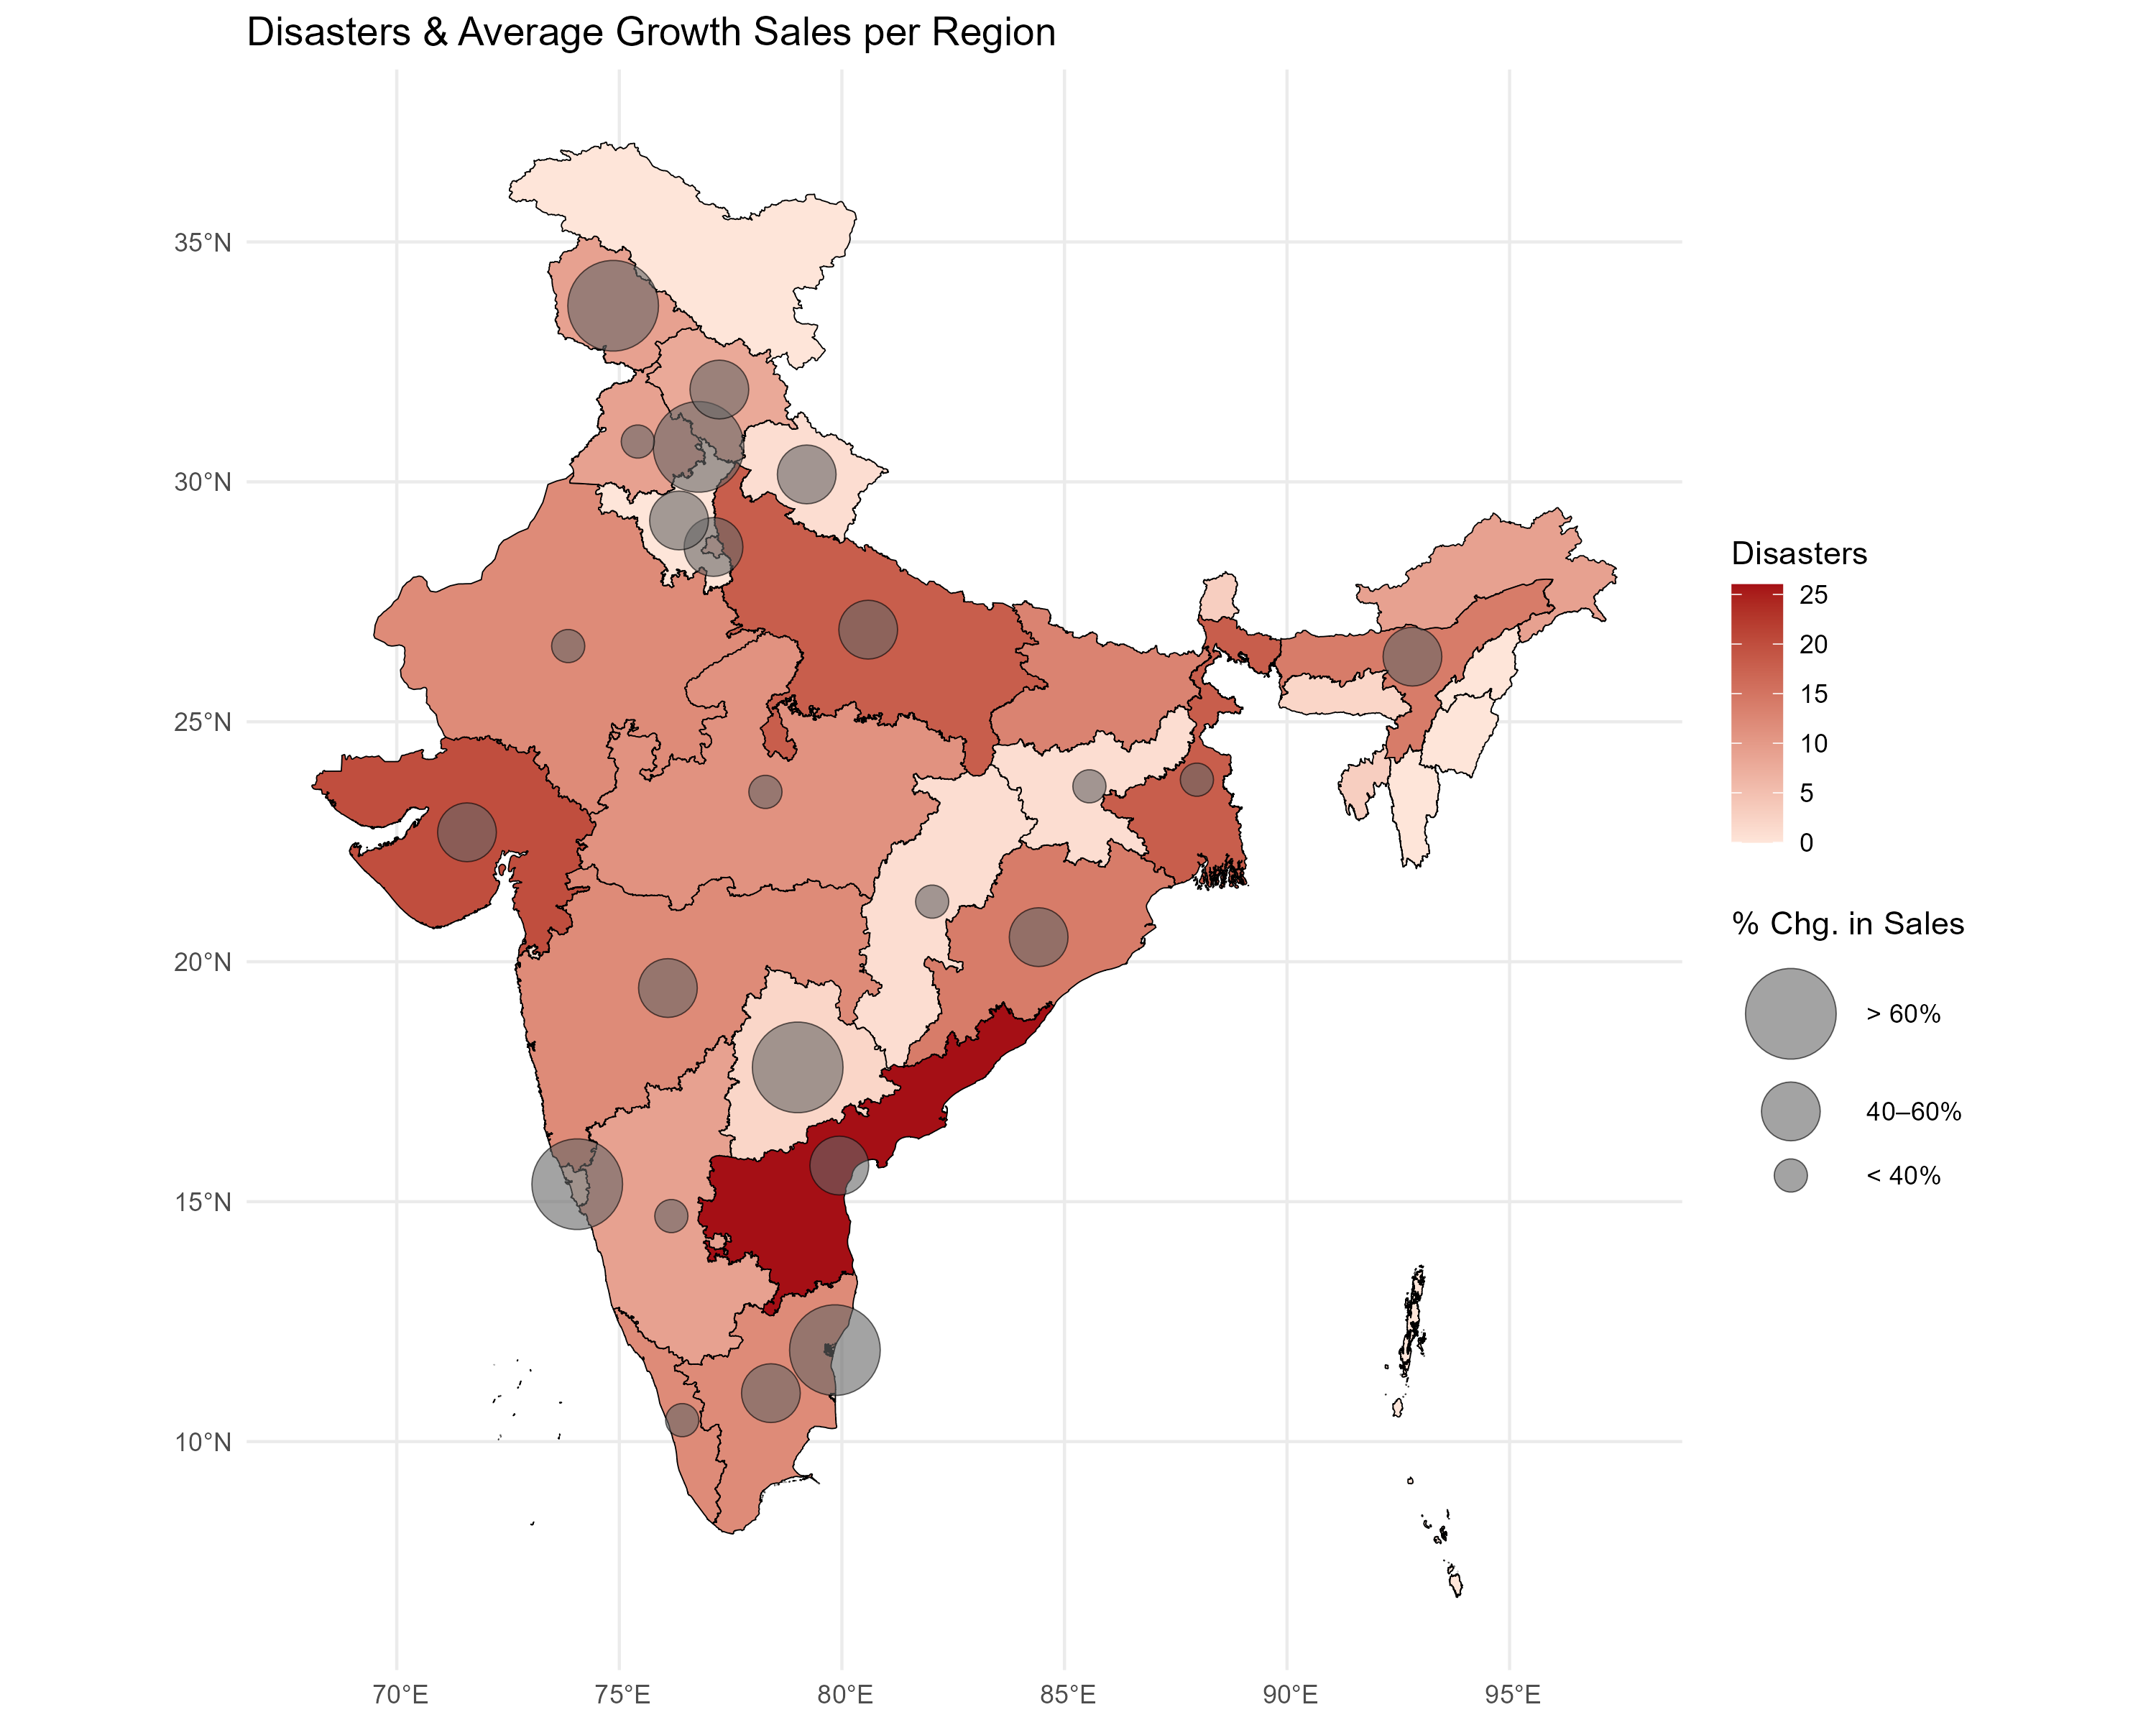
\includegraphics[width=1.2\linewidth]{disasters avgsales.png}
        \caption{Disasters per Region and Firms sales growth}
        \label{fig:Disastersmap}
    \end{figure}

Diving empirically into the problem is a way to ensure that there is or is not a clear effect. Since the effect is not clear, I will have to control for several factors to ensure that I can assess the impact of extreme disasters on firms. The next section will present extensively how I will isolate the impact of natural disasters on firm performance.

\newpage
\section{Empirical Strategy}

Isolating the impact of extreme natural disasters on firms can be a challenge, especially since we know that India has been the location of several natural disasters. In this section, I will clarify the methodology that I followed to estimate this effect while explaining the threats to identification that I faced. 

\subsection{\textit{An Event Study - Estimating the Aggregate Effect}}

\cite{Sun2021} demonstrated that to estimate the effect of several treatments (natural disasters in my case) on different groups (Indian states), a two-way fixed effects strategy could lead to several biases. They present an alternative framework, an event study. The underlying idea is to normalize all disasters to study the evolution of the treated and control groups before and after the disaster. The model presents itself as follows in Equation 1.

\begin{equation}
\text{lsales}_{it} = \sum_{t = -3,\, t \ne -1}^{5} \beta_t \cdot \text{disaster}_{kit}
+ \mathbf{X}_{it}'\boldsymbol{\gamma}
+ \alpha_i + \delta_{jt} + \psi_{gt} + \varepsilon_{it}
\end{equation}

The outcome variable being the logarithm of sales of a $\text{firm}_{i}$ in a $\text{year}_{t}$. The explanatory variables are a set of dummies ($\text{disaster}_{kit}$). First, there are immediate effect dummies that take the value of one if a firm was located during $\text{year}_{t}$ in the province where $\text{disaster}_{k}$ occurred. Then, there are the dummies that will represent the short- and medium-term effect of this $\text{disaster}_{k}$. They will take the value of one for each period $\text{t}_{+1}$,  $\text{t}_{+2}$ up to $\text{t}_{+5}$. The dummies for the period $\text{t}_{-3}$ and $\text{t}_{-2}$ will be used to estimate the presence of pretends that I will develop in the following section. Lastly, as a baseline for comparison, I will drop the period $\text{t}_{-1}$. The $\text{X}_{it}'$ is a vector of control variables at the levels $\text{firm}_{i}$ and $\text{year}_{t}$, such as productivity, energy expenses, and leverage ratio. I also control for non-time-varying firms' characteristics with firm fixed effect ($\alpha_i$), for sector time-varying characteristics with sector-year fixed effects ($\delta_{jt}$) and for group time-varying characteristics with ($\psi_{gt}$). There are several threats to the identification of the impact of extreme disasters on firms that I will address in the following sections.

\subsubsection{Spatial Autocorrelation and Conley Standard Errors}

Spatial correlation is a common threat in this kind of study. It often the case when the treatment is spatially distributed. The underlying idea is that treated firms are closer to each other because of their location. To test it, I will perform a Moran test to ensure that there is no spatial autocorrelation \citep{Moran1950,Kelejian2001}.
The Moran I statistic is 0.21 and is statistically significant at a 95\% confidence level. This means that firms with higher sales are located in provinces closer to provinces with firms with similar sales levels. Therefore, firms are not randomly distributed across space. Therefore, there is a need for spatial clustering. To do so, I follow the Conley specification with a clustering using latitudes and longitudes with a 690 km cutoff \citep{Conley1999,Conley2025}.

\subsubsection{Accounting for the presence of pre-trends}

Being able to successfully identify the impact of natural disasters on firms requires removing potential pretrends between the treatment and control groups. To be more specific, if the two groups followed different trends before the disaster took place, the treatment effect could be a reflection of previous differences. Figure \ref{fig:Pre-Trend graph} in the appendices clearly shows the presence of pretrends, at least for the period $\text{t}_{-3}$. To account for those, I decided to match my groups using the Propensity Score Matching (PSM) developed in \cite{Rosenbaum1983}. The characteristics chosen to create the score are productivity (tfp), energy expenses, leverage ratio, location (latitude \& longitude), and anticipation variables (developed in the following section). Using one of the most restrictive methods \textit{"nearest"}, the observations dropped from 26,133 to 8,830. Looking at the figure \ref{fig:PSM-PreTrend}, we can see that the pretrends for  $\text{t}_{-2}$ and  $\text{t}_{-3}$ are no longer significant. 
However, an important point to mention is that matching scores are effective when we got a clear exogenous treatment. In the context of this study, it is an issue that requires attention.  

\subsubsection{Dealing with anticipation behaviors}

103 natural disasters over a decade create anticipation behaviors that can alter the exogeneity of the impact of extreme disasters. Therefore, I created 3 anticipation variables for each broader type of disaster (storm, flood, drought). These variables are cumulative sums of smaller disasters by state. The underlying assumption is that firms located in provinces heavily affected by floods are more likely to adopt adaptation measures. These variables should control for these mechanisms. The equation of regression now includes these new variables.
\begin{align}
\text{lsales}_{it} =\ & \sum_{t = -3,\, t \ne -1}^{5} \beta_t \cdot \text{event}_{kit} + \omega \cdot \text{X}_{it}'\nonumber \\
&
+ \gamma_1 \cdot \text{droughts\_cumulative}_{pt}
+ \gamma_2 \cdot \text{floods\_cumulative}_{pt} \nonumber \\
& + \gamma_3 \cdot \text{cyclones\_cumulative}_{pt}
+ \alpha_i + \delta_{st} + \psi_{gt} + \varepsilon_{it}
\end{align}
Moreover, we could expect that some firms would change their location during the study period (1990-2006). However, after looking at switchers, I did not identify any firms that change location.

\subsection{\textit{Delving in the heterogeneity}}
As mentioned earlier, at an aggregated level, we do not find any significant effect of natural disasters on firm performance (Figure \ref{fig:Pre-Trend graph}). There could be several reasons. Some might experience the "Creative Destruction" that we mentioned and could alter the overall effect. To fully understand how firms react and to what extent they are affected by natural disasters, we need to disentangle the results. This subsection aims to present the strategy that I used and the mechanisms that I tested to better grasp this relationship.

\subsubsection{Importing foreign inputs}
Being part of a global value chain can be a source of uncertainty and risks. However, in the case of a domestic shock, such as extreme natural disasters, I expect firms that source their inputs on foreign markets to be less affected than other firms. To test this hypothesis, I will interact the explanatory variables of Equation 1 with a non-time-varying dummy variable that will take the value of one if the firm was importing a part of its input over the period of study. Equation 3 presents this new estimate.

\begin{align}
\text{lsales}_{it} =\ & \sum_{t = -3,\, t \ne -1}^{5} \beta_t \cdot \text{event}_{kit} * \text{ImpStatus}_{i} + \omega \cdot \text{X}_{it}'\nonumber \\
&
+ \gamma_1 \cdot \text{droughts\_cumulative}_{pt}
+ \gamma_2 \cdot \text{floods\_cumulative}_{pt} \nonumber \\
& + \gamma_3 \cdot \text{cyclones\_cumulative}_{pt}
+ \alpha_i + \delta_{st} + \psi_{gt} + \varepsilon_{it}
\end{align}

Then, since I have information on the type of inputs imported (raw materials, intermediate inputs, finished goods). I will look at how the type of input imported helps the most when a firm faces extreme natural disasters. The variable $\text{ImpStatus}_{i}$  will now take the value of one if a firm imports raw materials, intermediate inputs, or finished goods.

\subsubsection{Differences across Industries}
By the nature of their activity, firms will be more or less harmed by extreme natural disasters. Firms in the agricultural industry are known to be greatly affected by floods or storms. The seasonality of their activity creates a vulnerability from which it could take more time to recover compared to other firms. In contrast, depending on the intensity of the shock, companies in the machinery or chemicals sectors should be less affected by these disasters. To test these hypotheses, I follow the same framework presented in the previous subsection, using industries as interaction variables. As a baseline for comparison, the Chemicals and Minerals category will be dropped in the estimations. Indeed, it is a relatively stable industry, located in a central location in the value chain.   
\begin{align}
\text{lsales}_{it} =\ & (\sum_{t = -3,\, t \ne -1}^{5} \beta_t \cdot \text{event}_{kit}) *( \text{Primary}_{i}+ \text{LightManuf}_{i}+ \text{Machinery}_{i} + \text{ChemMin}_{i} + \text{Other}_{i}) + \omega \cdot \text{X}_{it}'\nonumber \\
&
+ \gamma_1 \cdot \text{droughts\_cumulative}_{pt}
+ \gamma_2 \cdot \text{floods\_cumulative}_{pt} \nonumber \\
& + \gamma_3 \cdot \text{cyclones\_cumulative}_{pt}
+ \alpha_i + \delta_{st} + \psi_{gt} + \varepsilon_{it}
\end{align}

\section{Results}

\subsection{\textit{Main Results}}

As developed in figures \ref{fig:Pre-Trend graph} and \ref{fig:PSM-PreTrend} in the appendices, the matching method fixed the pre-trend issue but did not produce significant results on the impact of extreme natural disasters on firm sales at an aggregated level. Identifying a significant result at an aggregate level can be a challenge in our context. The literature has shown that extreme disasters can also positively impact the economy; this is the \textit{"Creative Destruction"} theory \citep{Leiter2009,Fatica2024,RothTran2025}. This could partly explain the non-significant findings in figure \ref{fig:PSM-PreTrend}. However, studying this relationship at an aggregate level may lead to incomplete conclusions. Previous research has shown that disasters have heterogeneous effects on firms \citep{Bas2025, Nedoncelle2024}. Therefore, a dive into the heterogeneity is essential to fully capture this relationship. 

\subsubsection{Who are the most at risk?}

Some industries are more at risk in the event of natural disasters. Previous studies have shown that firms in the upstream industries are more sensitive to climatic conditions \citep{Barattieri2023,Okubo2021}. Figure \ref{fig:BaselinePrim} confirms this theory. The figure clearly shows the immediate impact of extreme natural disasters on firms in Primary \& Processed products industry. They experience a significant decrease in their sales compared to both the baseline industry (Chemicals and minerals) and to firms in Primary \& Processed products industries that were not affected by a disaster. Moreover, this drop in sales holds for the two years following the disaster. This is consistent with the work of \cite{Tanaka2015, Lai2022,Zhou2021,Berkel2021} that found that there is a clear negative impact of natural disasters in the short term.

\begin{figure}[H]
        \centering
        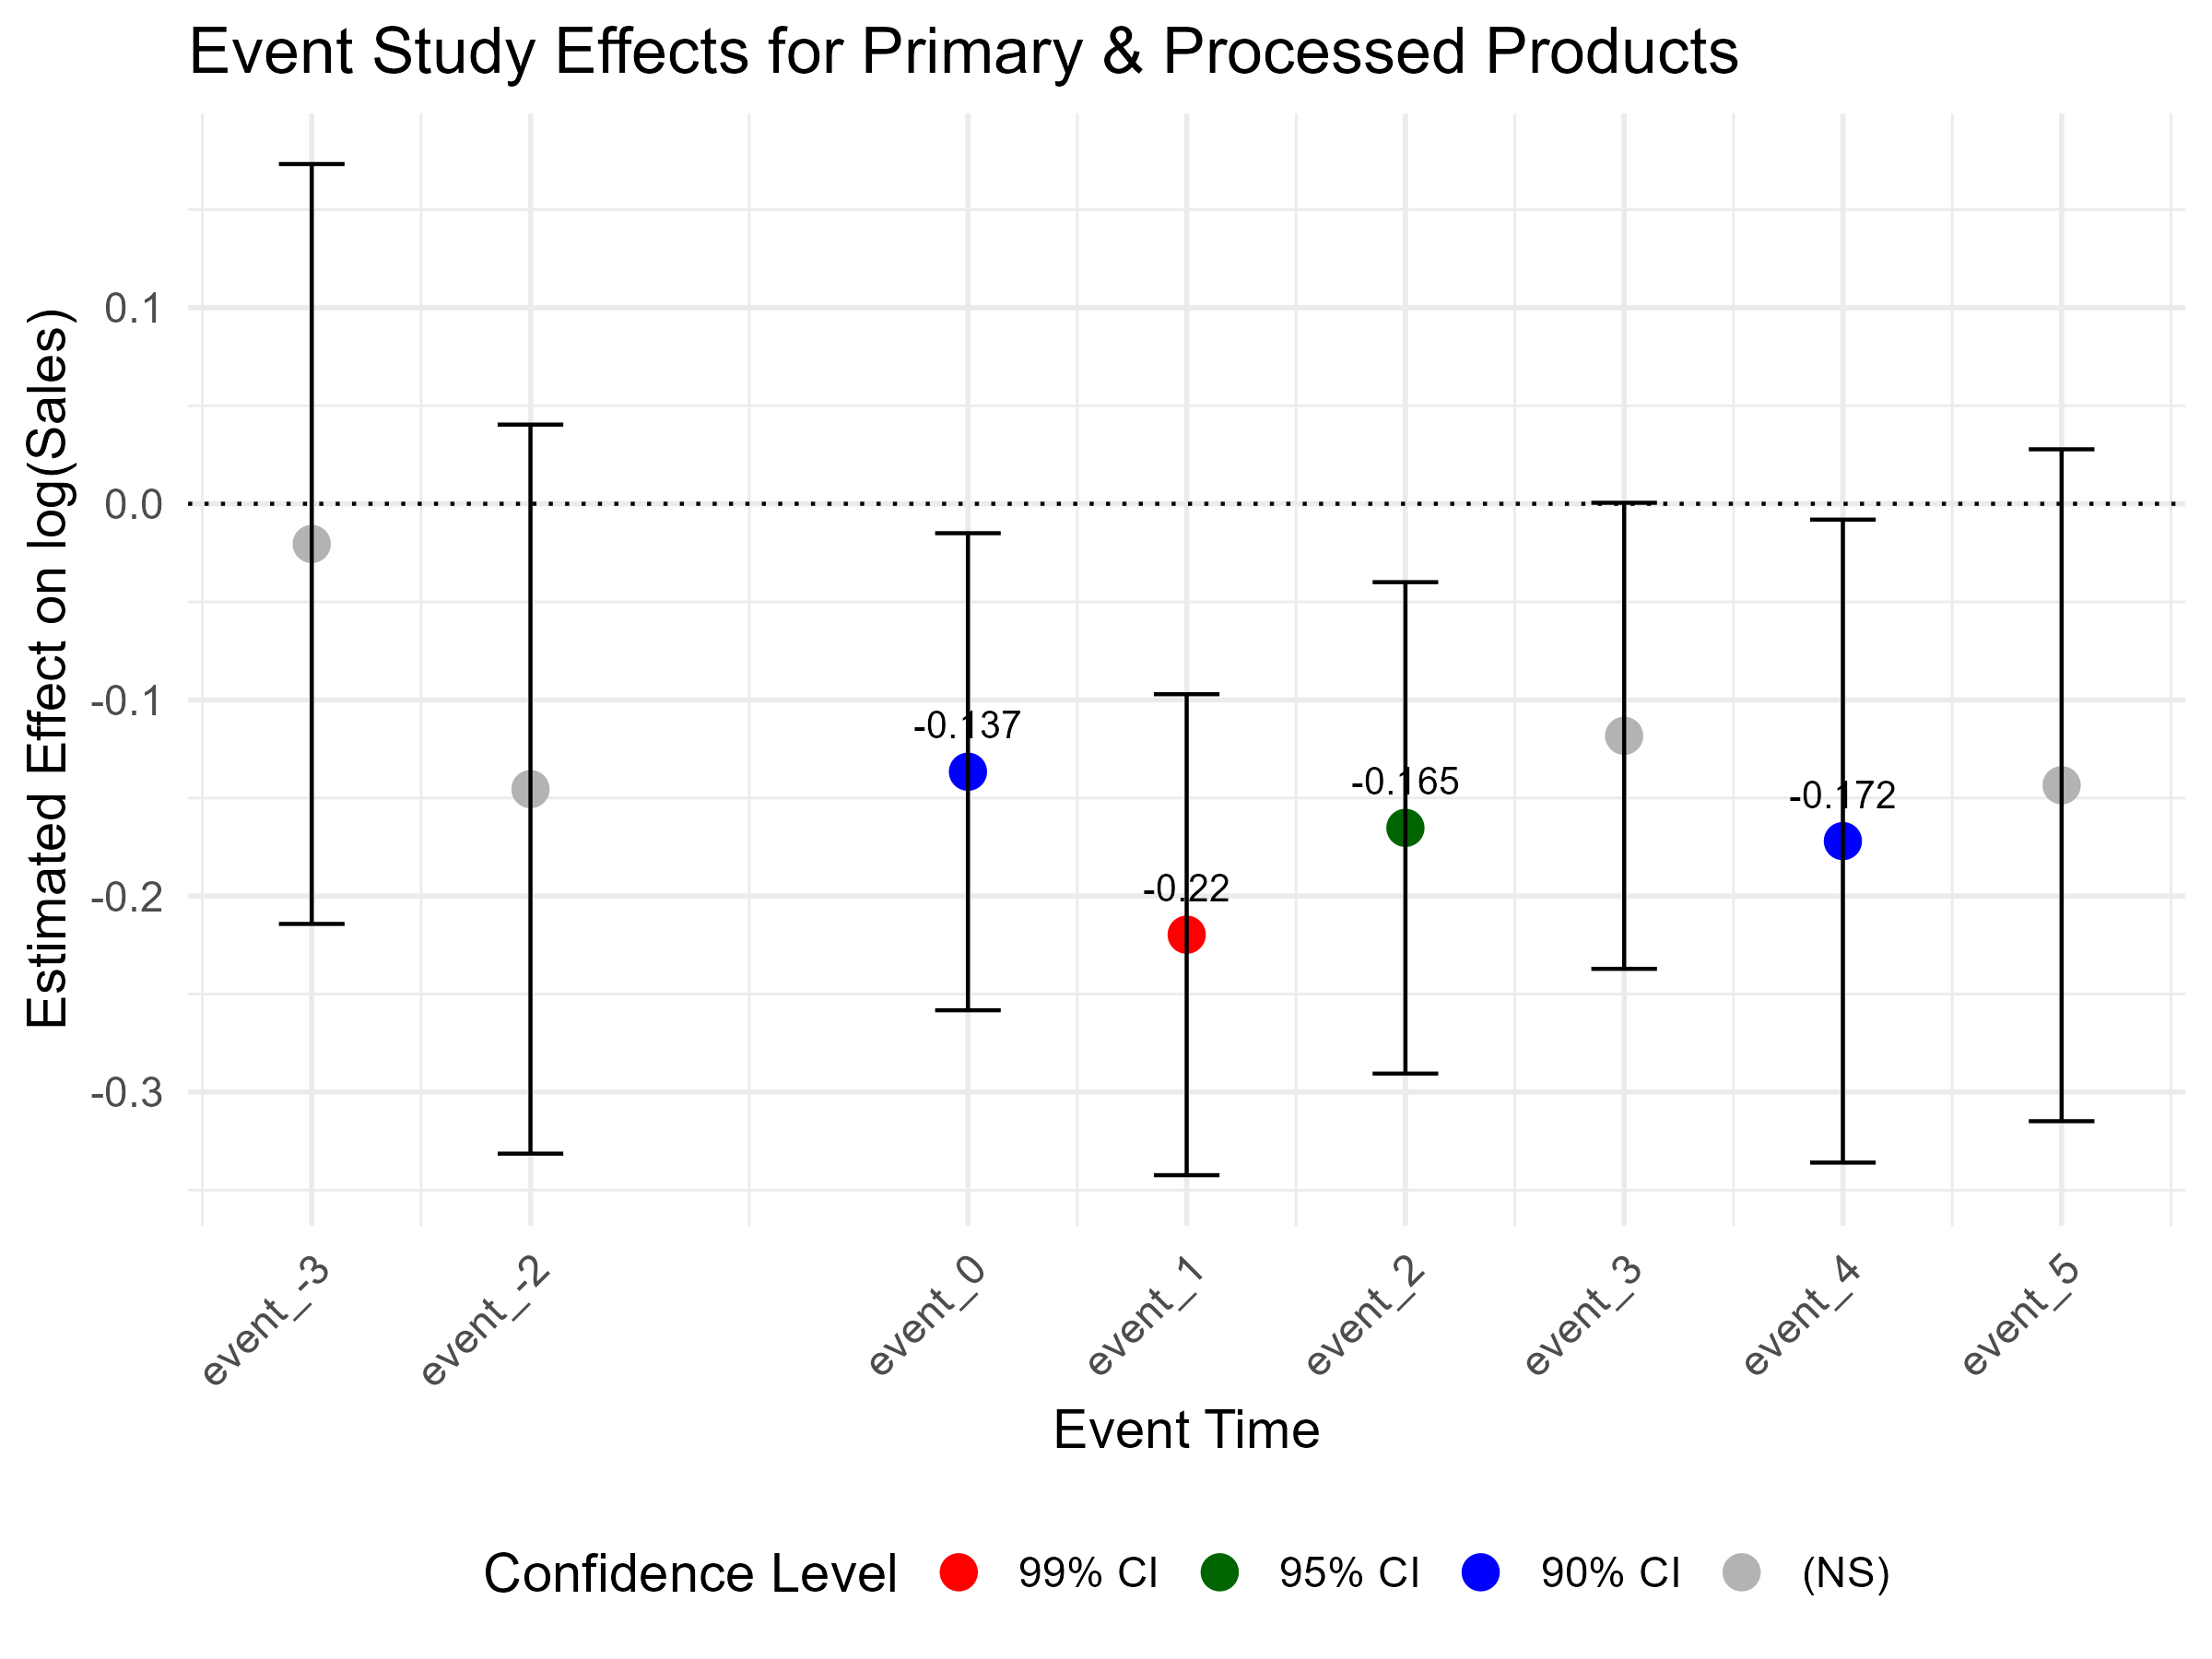
\includegraphics[width=0.55\linewidth]{BaselinePrim.png}
        \caption{Impact of Extreme Natural Disasters on Primary \& Processed Products firms}
        \label{fig:BaselinePrim}
    \end{figure}

In terms of magnitude, column 2 of Table \ref{tab:event_sector_interaction_trend} presents the impact of natural disasters compared to firms in the chemical and mineral industry. In the year of the disaster, their sales decrease on average by 13.6\% compared to the baseline industry. This loss becomes even more important the following year with an average drop of 22\% of their sales, all other things being kept equal. Firms in primary \& processed goods industry will suffer up to four years after the disaster.  Now, compared to their siblings that are in the same industry but were not affected by these disasters, these companies experienced a drop in their sales of 7.9\% on average in the year of the disaster. This effect falls to 10.8\% on average in the second year and stabilizes around 5\% until four years after the disaster.

\begin{figure}[H]
        \centering
        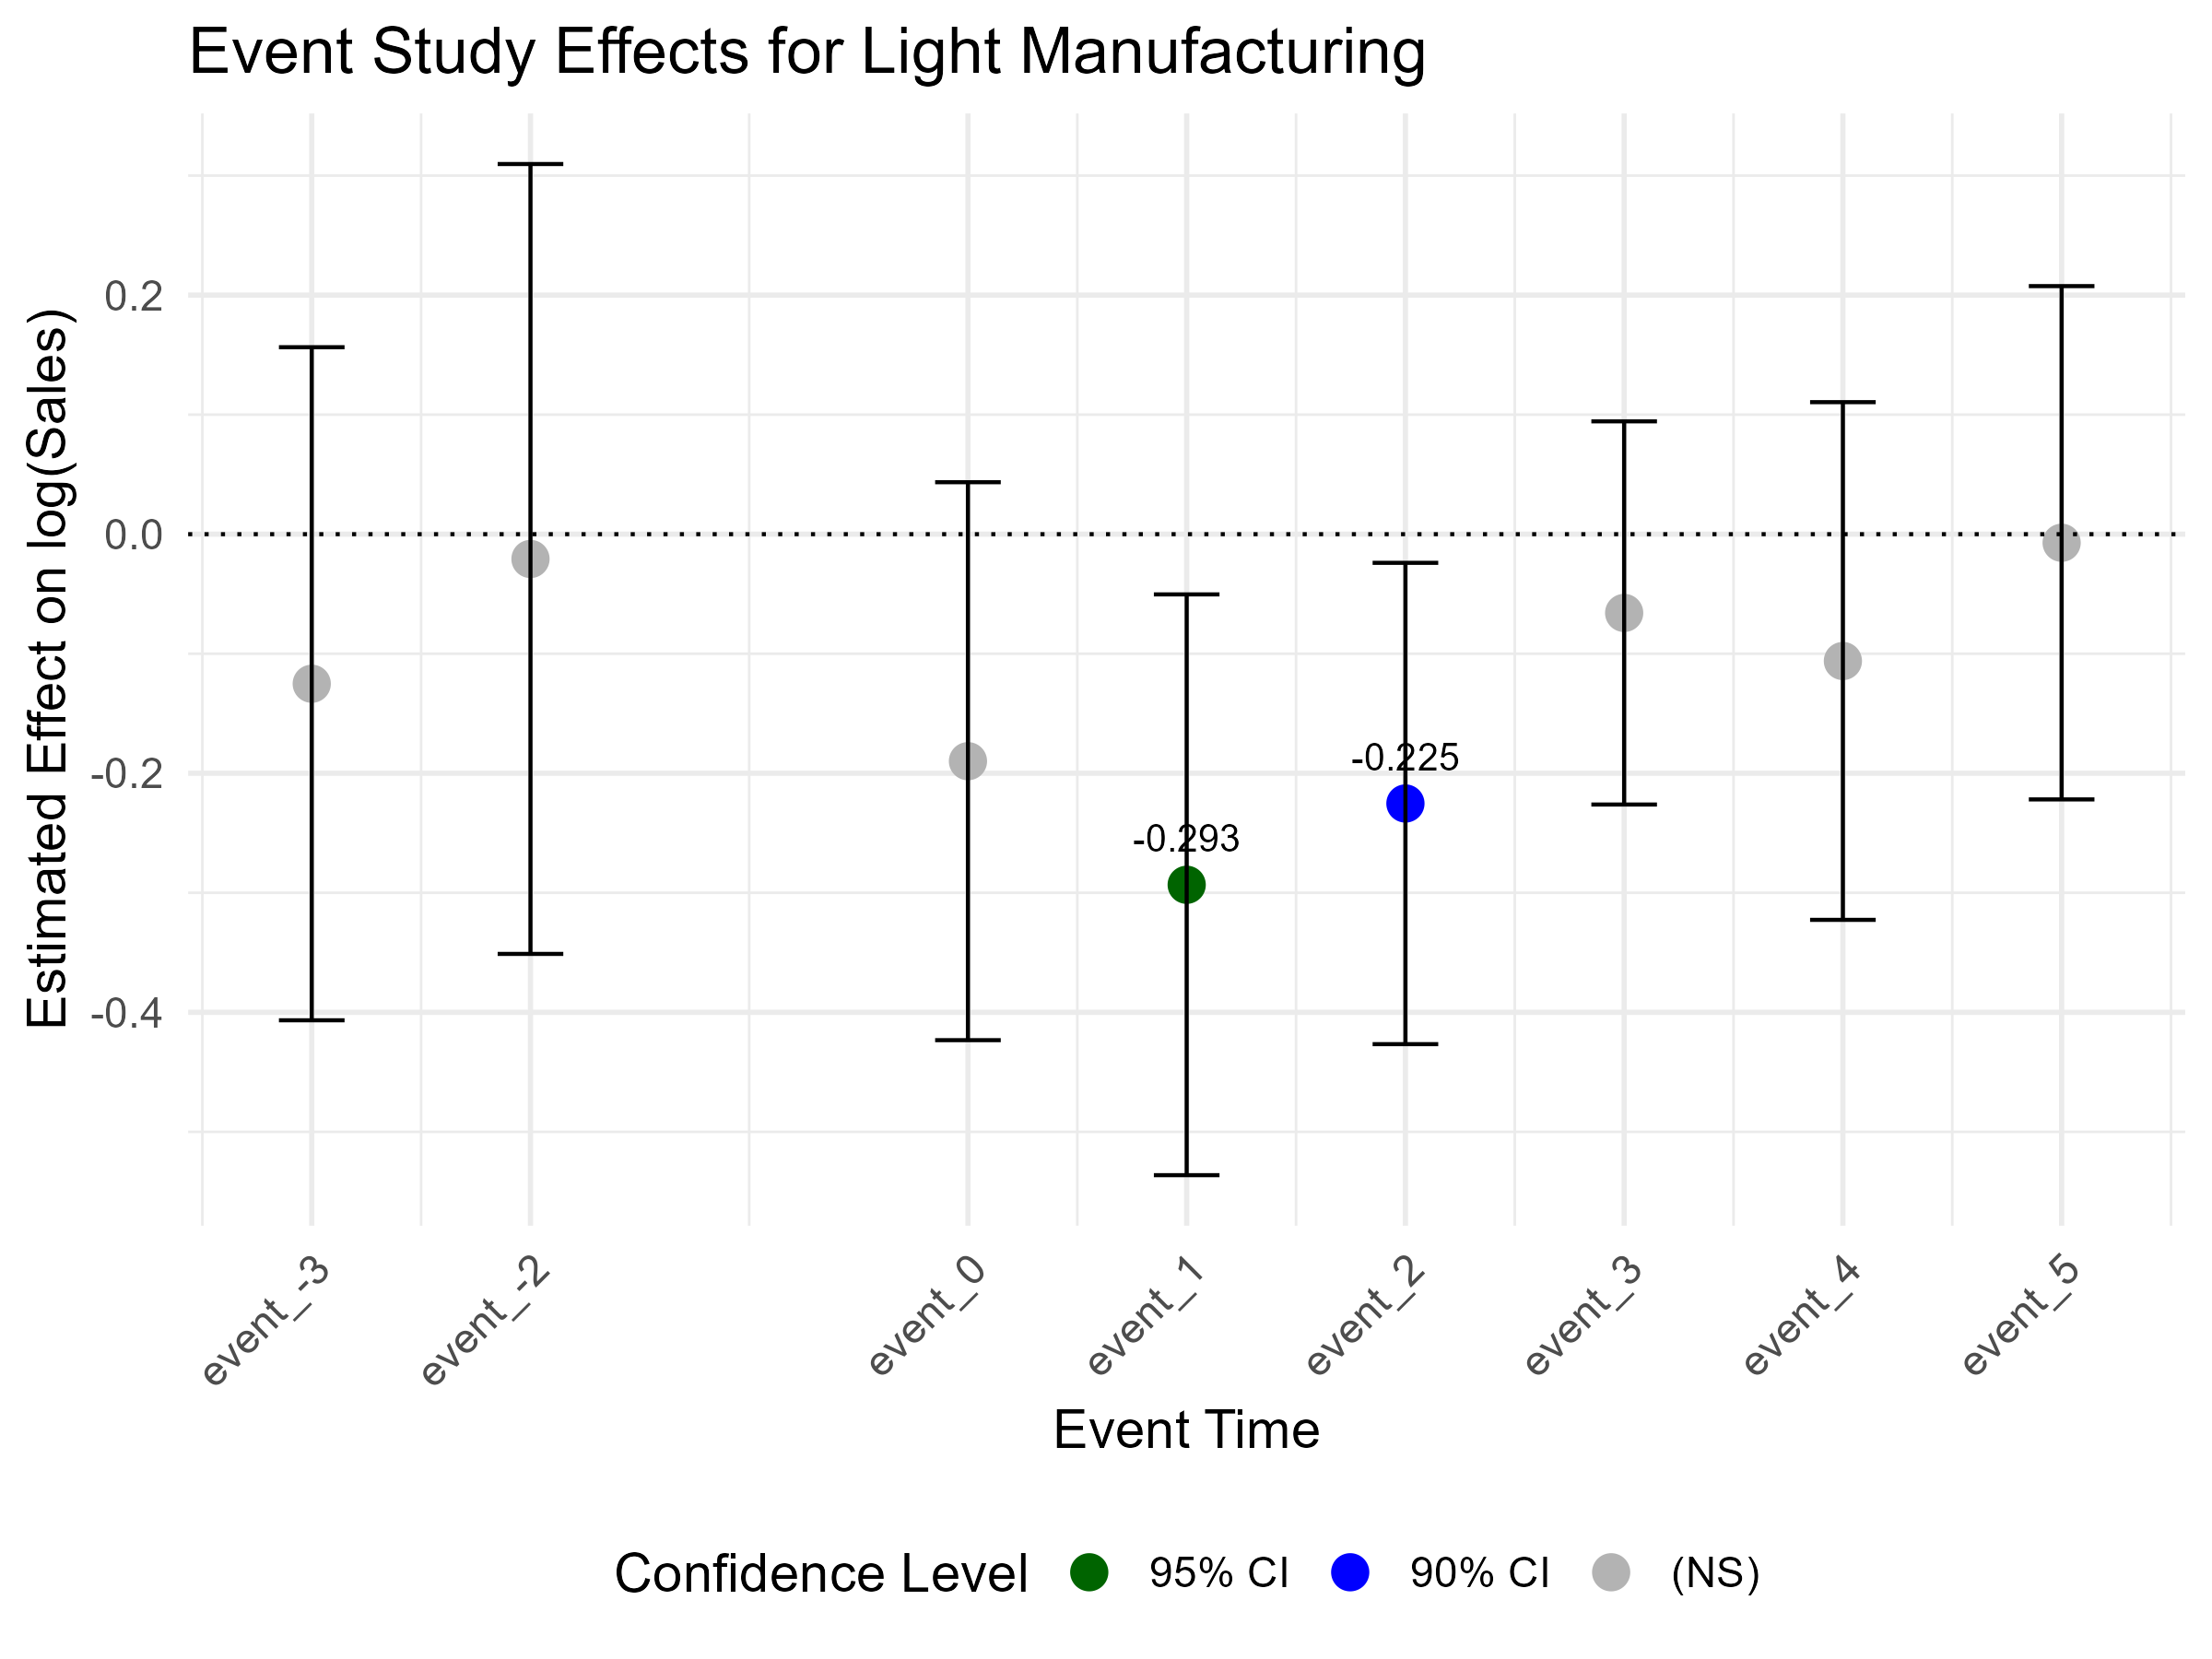
\includegraphics[width=0.55\linewidth]{BaselineLightManuf.png}
        \caption{Impact of Extreme Natural Disasters on Light Manufacturing firms}
        \label{fig:LightManuf}
    \end{figure}

Firms in the Light Manufacturing industry are also impacted. The third column of Table \ref{tab:event_sector_interaction_trend} presents the magnitude of this loss. In the year of disasters, firms in the light manufacturing industry experienced on average a decrease 19\% of their sales compared to those in the chemical and mineral industries. Compared to firms that are not affected by natural disasters, this drop in sales is on average about 15\%. The losses hold only in the short term ($\text{t}_{+1}$, $\text{t}_{+2}$) as we can see on the graph (\ref{fig:LightManuf}). In these periods,  these firms saw their sales decrease by 18\% in ($\text{t}_{+1}$) and 9\% in ($\text{t}_{+2}$) compared to the baseline industry. Light manufacturing firms are able to recover from these losses in the medium term, as we can observe that the effect is no longer significant for these periods ($\text{t}_{+3}$, $\text{t}_{+4}$, $\text{t}_{+5}$) compared to firms in the light manufacturing industry that were not affected by disasters. However, we observe a negative and significant decrease even in $\text{t}_{+3}$ and $\text{t}_{+4}$ compared to those in the baseline category. 

\begin{table}[H]
    \centering
    \small
    \caption{Event Study with Sector Interactions on Log Sales}
    \resizebox{\textwidth}{!}{
    \begin{threeparttable}
    \begin{tabular}{lccccc}
    \toprule
     & Main Effect & Primary \& Processed & Light Manufacturing & Machinery \& Capital & Other \\
    \cmidrule{2-6}
     \textit{Estimation Results} & (1) & (2) & (3) & (4) & (5) \\
    \midrule
    \textit{\textbf{Immediate Impact}} \\
    Event t+0   & 0.0582* & -0.1366*** & -0.1899*** & 0.0162 & -0.0283 \\
              & (0.0252) & (0.0288) & (0.0253) & (0.0339) & (0.0230) \\
    \midrule
    \textit{\textbf{Short term}} \\
    Event t+1   & 0.1104** & -0.2197*** & -0.2933*** & -0.0306 & -0.1683*** \\
              & (0.0418) & (0.0168) & (0.0388) & (0.0344) & (0.0383) \\
    Event t+2   & 0.1311*** & -0.1653*** & -0.2253*** & -0.0553. & -0.1719*** \\
              & (0.0256) & (0.0490) & (0.0391) & (0.0306) & (0.0228) \\
    \midrule
    \textit{\textbf{Medium/Long term}} \\
    Event t+3   & 0.0604*** & -0.1183*** & -0.0659*** & -0.0117 & -0.0770*** \\
              & (0.0034) & (0.0350) & (0.0145) & (0.0108) & (0.0042) \\
    Event t+4   & 0.0609. & -0.1720*** & -0.1061** & 0.0364* & 0.0680 \\
              & (0.0313) & (0.0520) & (0.0400) & (0.0160) & (0.0496) \\
    Event t+5   & 0.0297 & -0.1435. & -0.0072 & 0.0537*** & 0.0790* \\
              & (0.0301) & (0.0769) & (0.0680) & (0.0092) & (0.0402) \\
    \midrule
    \textit{\textbf{Controls}} \\
    Productivity (tfp) & \multicolumn{5}{c}{0.7008***} \\
     & \multicolumn{5}{c}{(0.0301)} \\
    Log Leverage Ratio & \multicolumn{5}{c}{- 0.2989***} \\
     & \multicolumn{5}{c}{(0.0616)} \\
     Log Energy expenses & \multicolumn{5}{c}{0.6870***} \\
      & \multicolumn{5}{c}{(0.0121)} \\
     Droughts cumulative & \multicolumn{5}{c}{0.0010} \\
      & \multicolumn{5}{c}{(0.0160)} \\
     Floods cumulative & \multicolumn{5}{c}{0.0242***} \\
      & \multicolumn{5}{c}{(0.0058)} \\
     Cyclones cumulative & \multicolumn{5}{c}{- 0.0244***} \\
      & \multicolumn{5}{c}{(0.0081)} \\
      \midrule
    \textbf{Fixed Effects} & \multicolumn{5}{c}{Firm + Industry-Year + Group-Year} \\
    \textbf{Standard Errors} & \multicolumn{5}{c}{Conley (690 km)} \\
    \textbf{Observations} & \multicolumn{5}{c}{8,830} \\
    \textbf{R\textsuperscript{2}} & \multicolumn{5}{c}{0.96492} \\
    \textbf{Within R\textsuperscript{2}} & \multicolumn{5}{c}{0.59918} \\
    \bottomrule
    \end{tabular}
    \begin{tablenotes}
        \small
        \item \textit{Notes:} Columns 2-5 represents the estimated coefficients of the differential impact of natural disasters on treated firms in each sector, relative to both (i) non-treated firms in the same sector and (ii) treated firms in the baseline sector (Chemicals and Minerals in column 1).Conley-adjusted standard errors (in parentheses) for the main effect and its interaction with sector group dummies.
        Control variables include: TFP, leverage, electricity use, total assets, cumulative droughts, floods, and cyclones.
        The omitted (baseline) industry is \textbf{Chemicals and Minerals}.
        \textbf{***} $p<0.001$, \textbf{**} $p<0.01$, \textbf{*} $p<0.05$, \textbf{.} $p<0.1$.
    \end{tablenotes}
    \end{threeparttable}
    }
    \label{tab:event_sector_interaction_trend}
\end{table}


Machinery and Capital goods firms should be in theory more resilient to extreme natural disasters. This is what I also observe in the fourth column of Table \ref{tab:event_sector_interaction_trend} and in Figure \ref{fig:BaselineMachin}. In the immediate and short term, I do not observe any significant impact of the shock on these firms. However, I notice a positive and significant effect only compared to the baseline for the periods $\text{t}_{+4}$ and $\text{t}_{+5}$ on average 3\% and 5\%. The results for the "Other" industry can be found in the appendices in Figure \ref{fig:BaselineOthers}.

\begin{figure}[H]
        \centering
        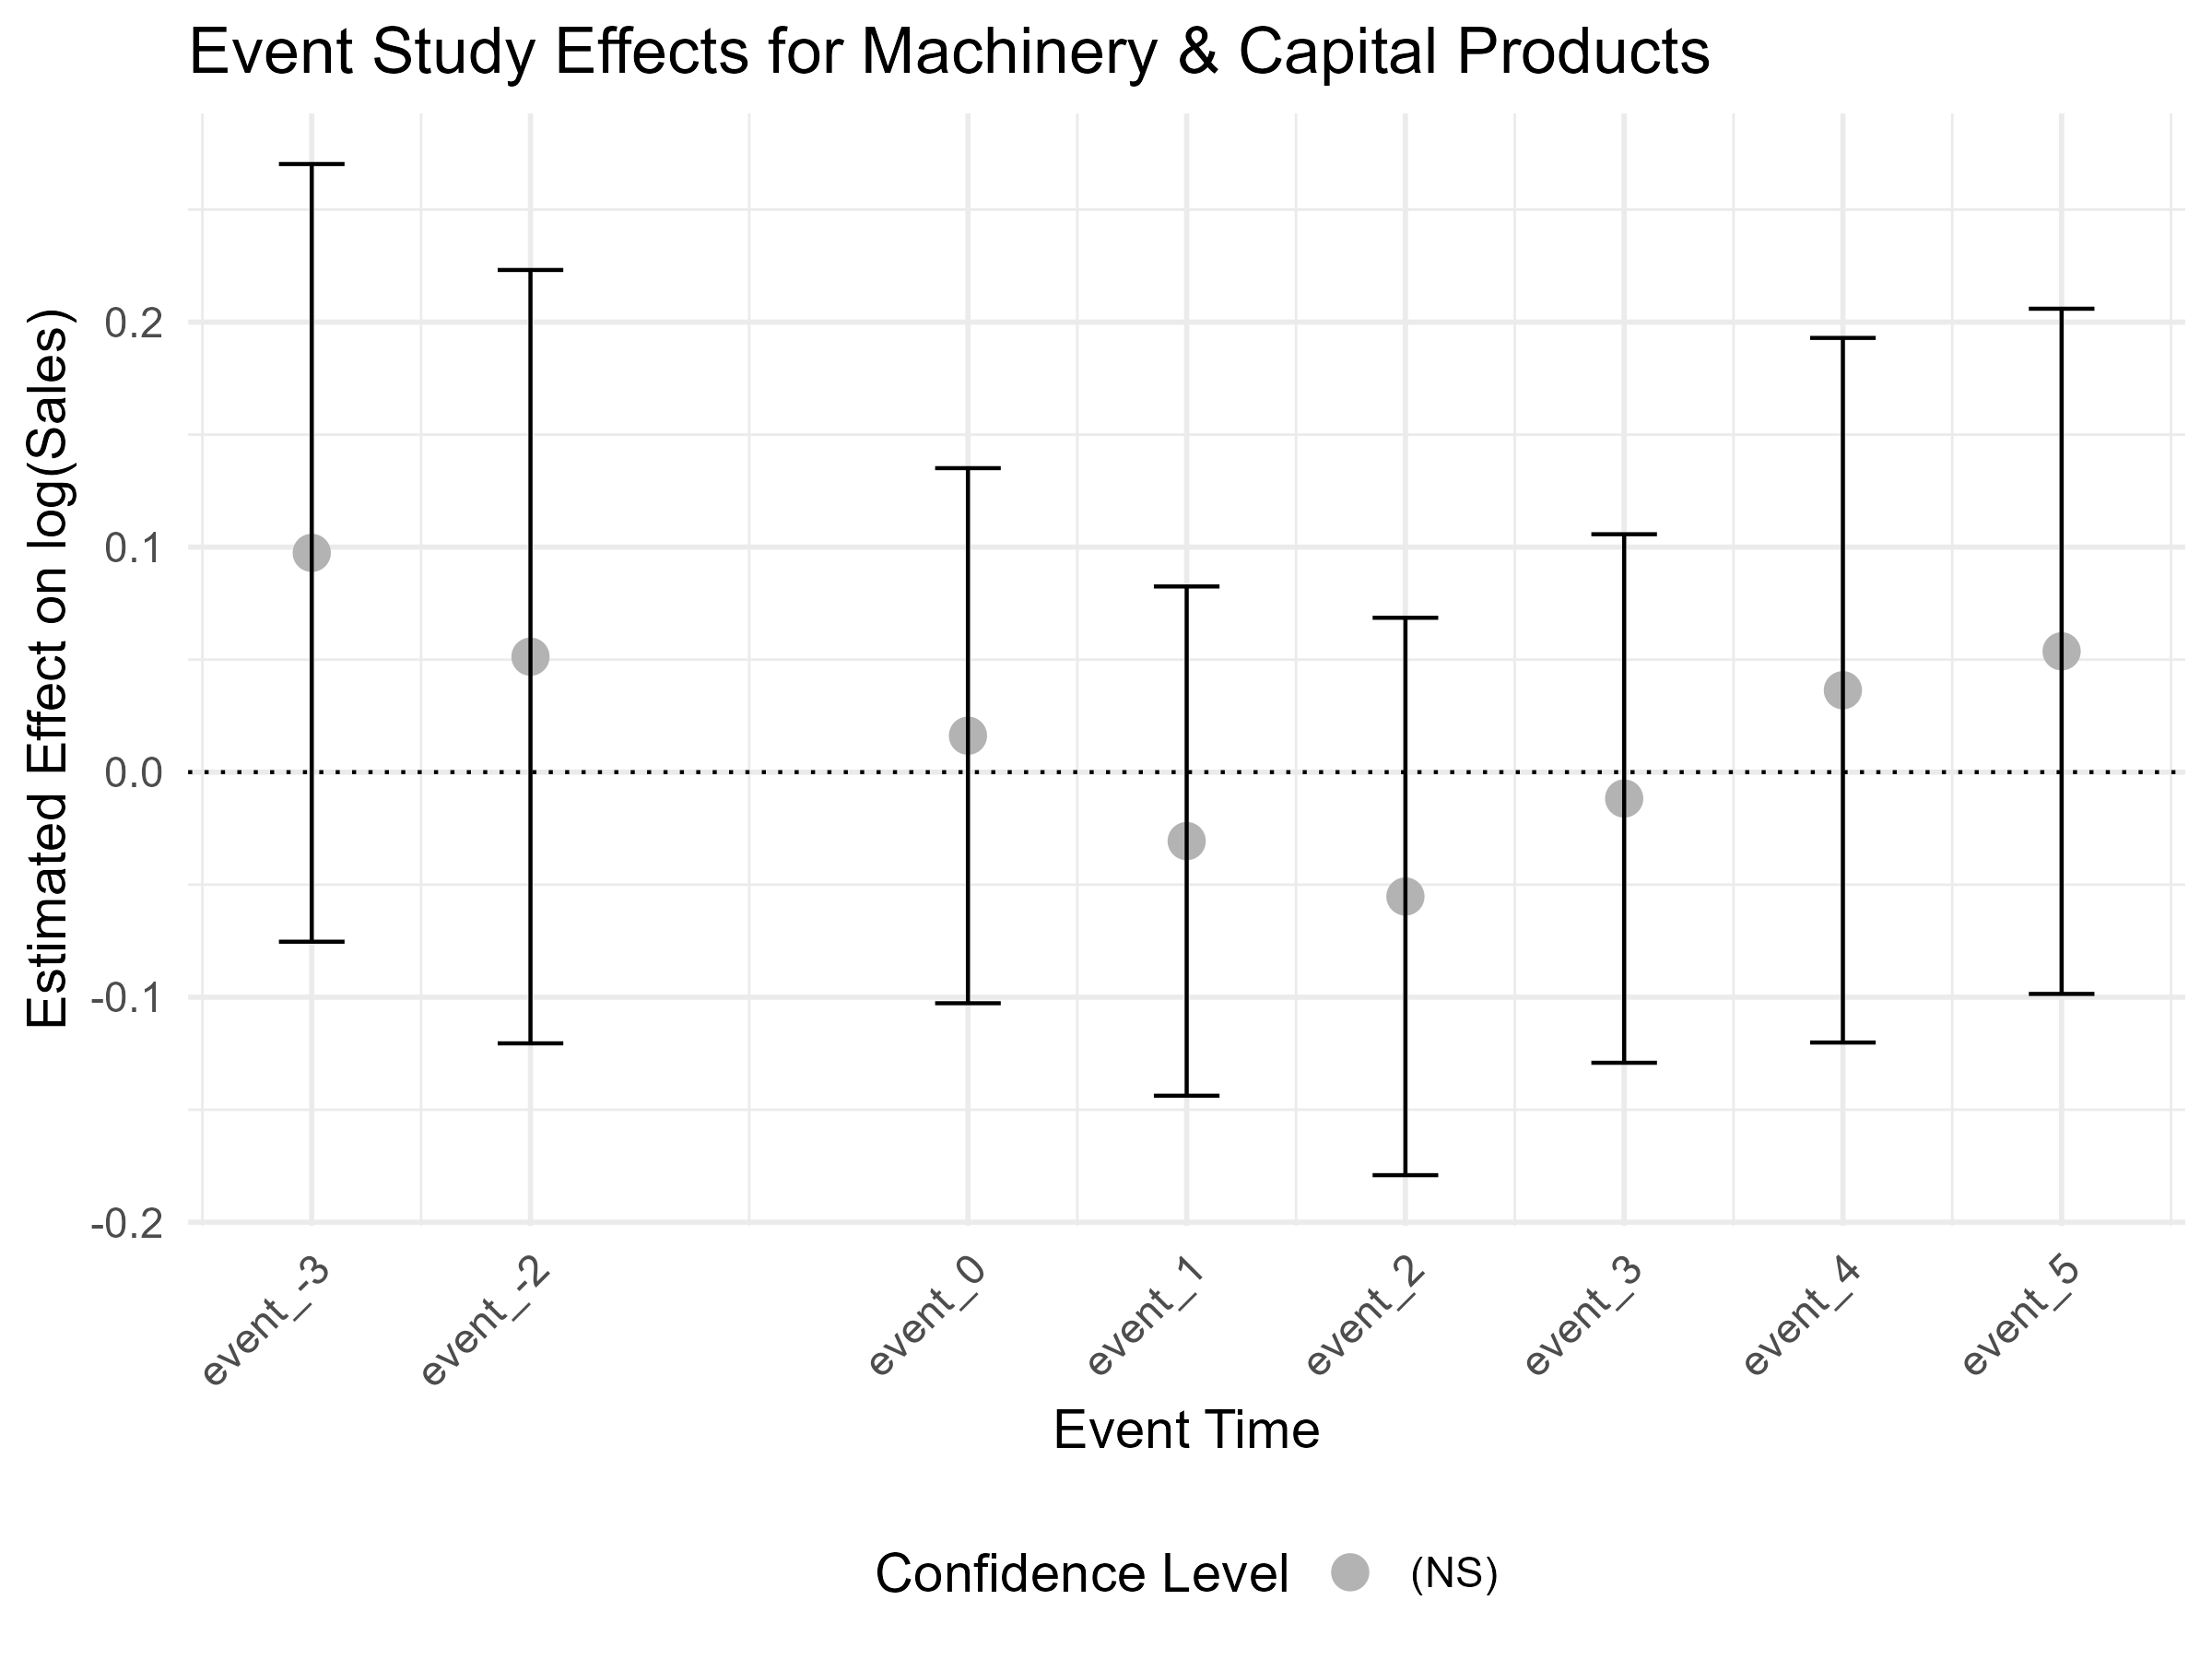
\includegraphics[width=0.55\linewidth]{BaselineMachinery.png}
        \caption{Impact of Extreme Natural Disasters on Light Manufacturing firms}
        \label{fig:BaselineMachin}
    \end{figure}

\subsubsection{The role of imported inputs in mitigating extreme disasters}

By nature, an extreme natural disaster is a relatively local phenomenon. Therefore, foreign inputs can reduce extreme disaster damage. Looking at Figure \ref{fig:Imp}, we can see that compared to other firms, Importers are better off. Their sales increase in the short and medium term after a disaster. Column 5 of Table \ref{tab:main_interactions} shows that compared to firms that do not import (but are affected by a natural disaster), importers experience a significant increase in their sales of about 10.5\% on average in the year after the disaster. This increase holds for the four following years about 5\% in $\text{t}_{+2}$, 8.9\% in $\text{t}_{+3}$ and 7\% in $\text{t}_{+4}$ on average. The baseline coefficients can be found in the Appendices (\ref{tab:main_interactions_baseline}); this will allow comparison with importers that were not affected by natural disasters. Compared to non-affected importers, this increase effect is lower in magnitude but still significant. The increase in sales is about 4.2\% in $\text{t}_{+1}$, 4.9\% in $\text{t}_{+2}$, 4.3\% in $\text{t}_{+3}$, and 6.8\% in $\text{t}_{+4}$.


\begin{figure}[H]
        \centering
        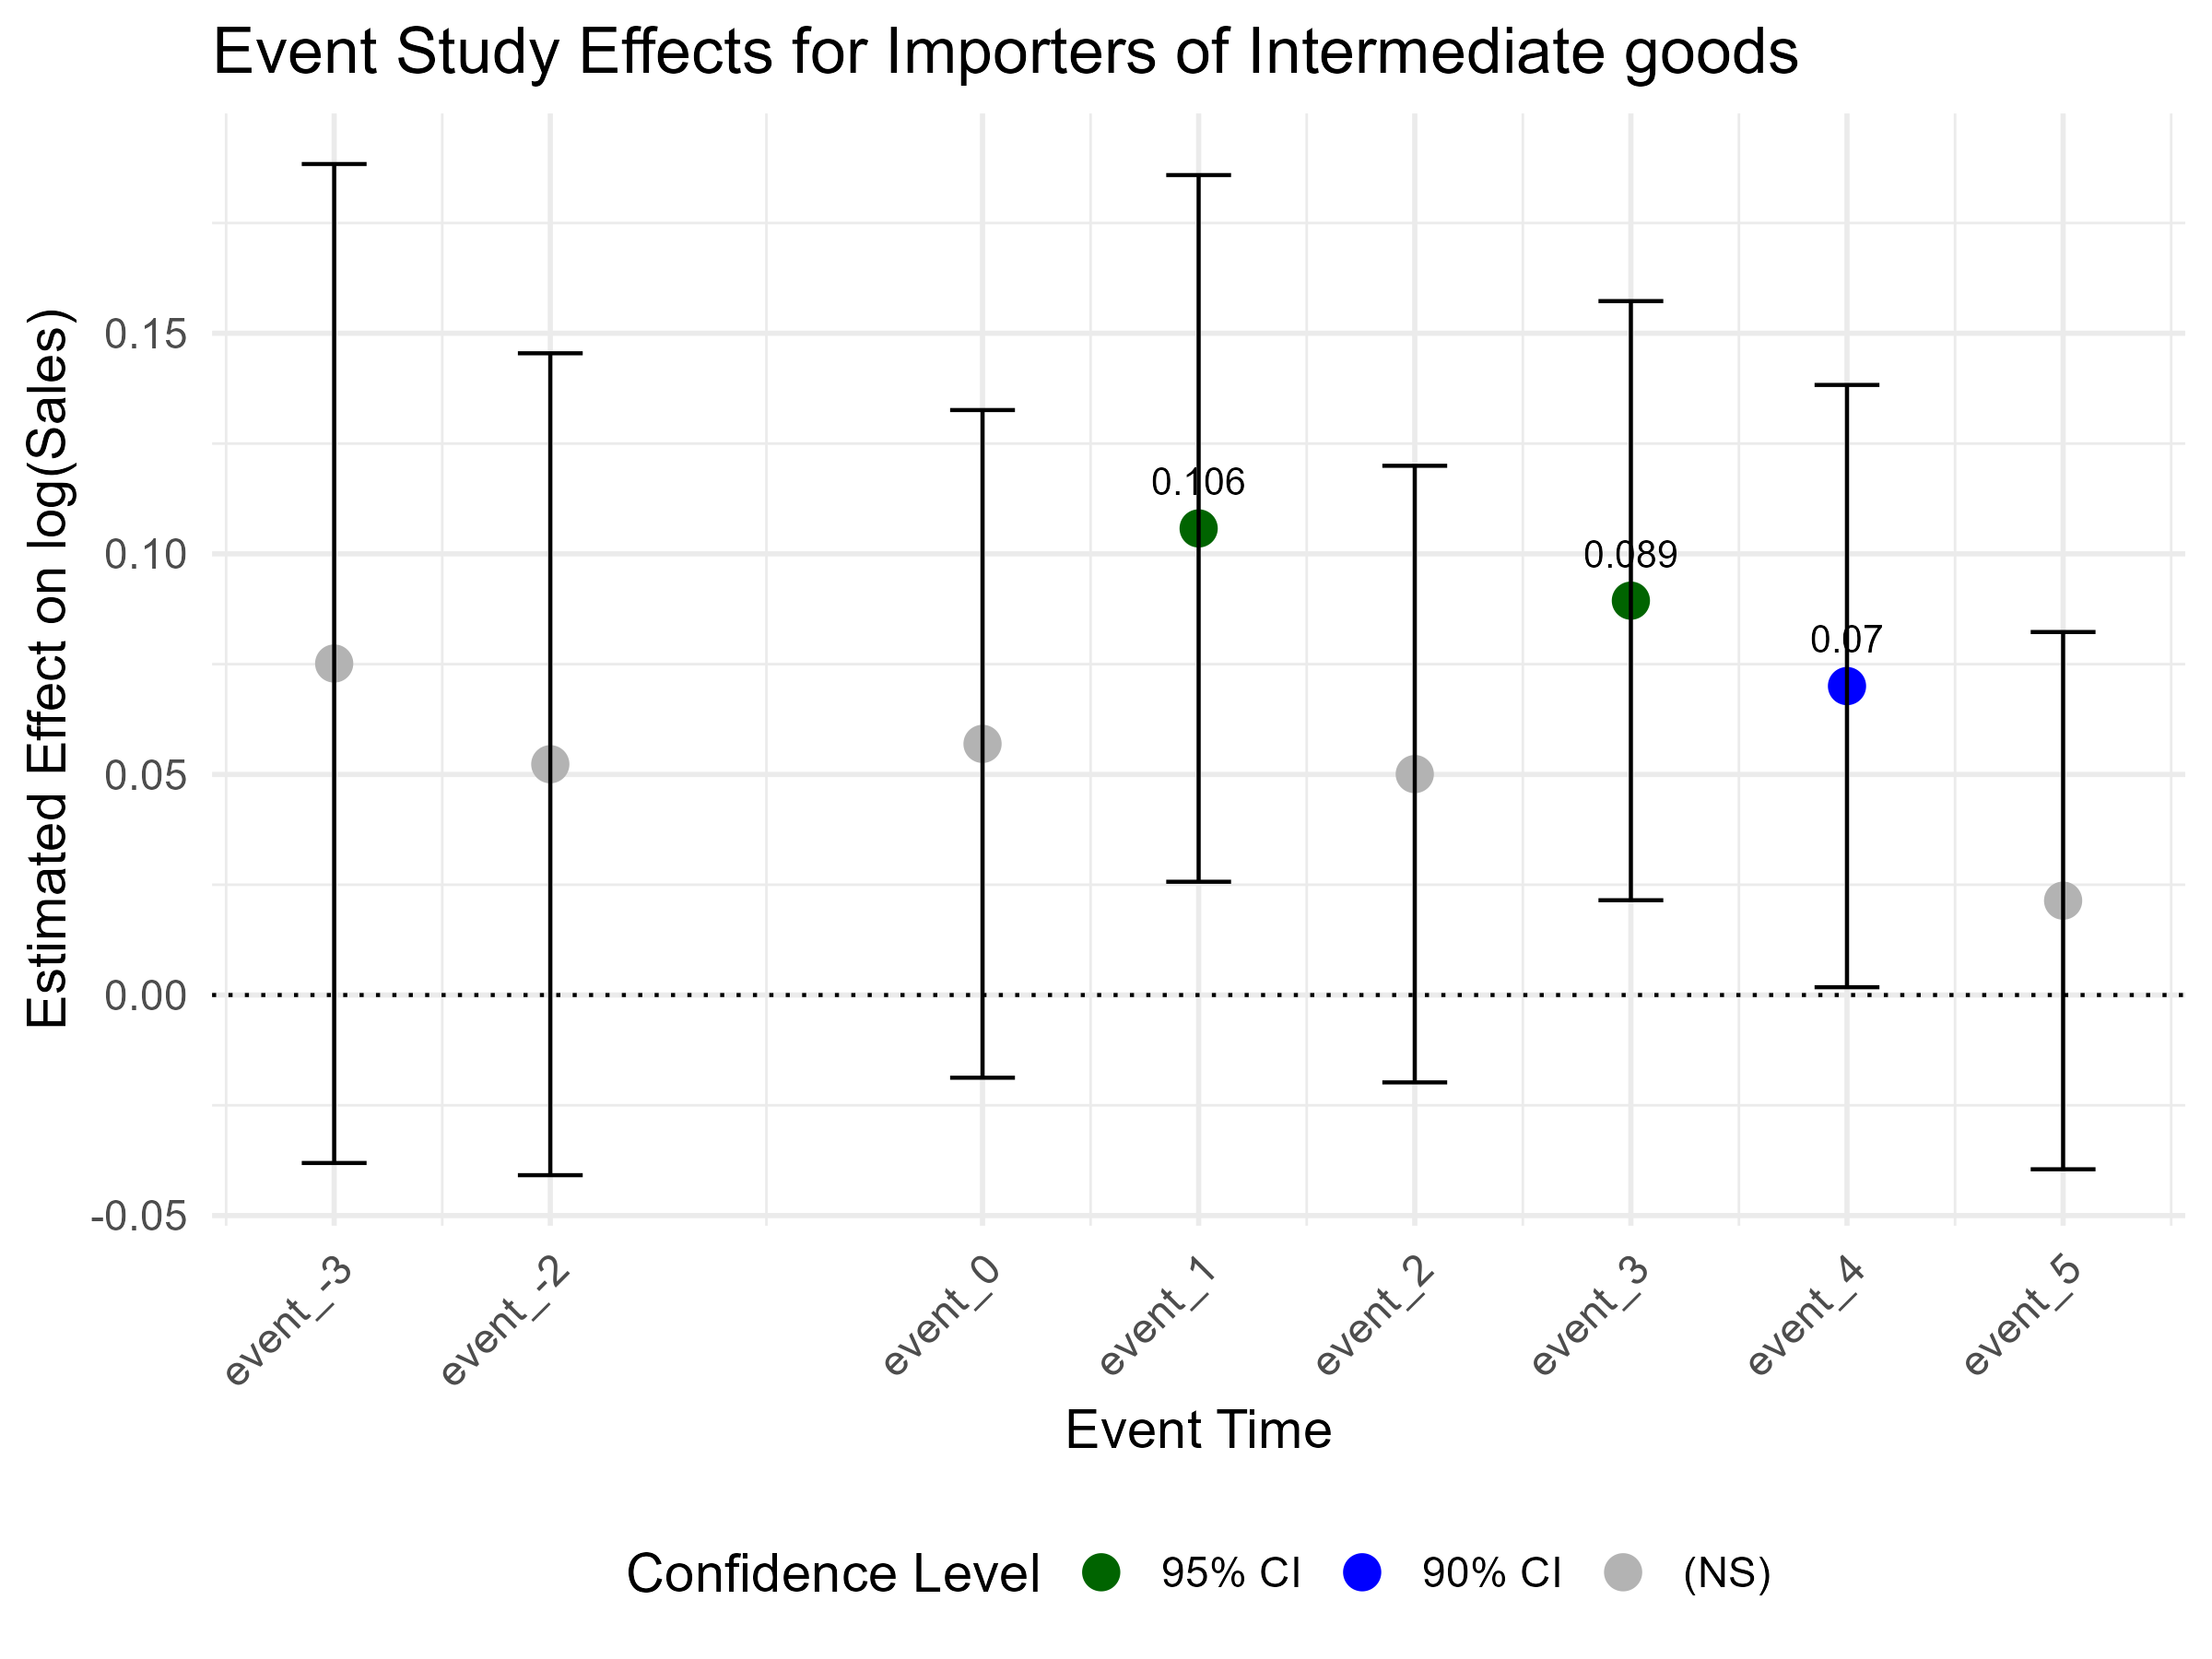
\includegraphics[width=0.55\linewidth]{Importer.png}
        \caption{Impact of Extreme Natural Disasters on Firms that source their inputs abroad}
        \label{fig:Imp}
    \end{figure}

We have stated that being an importer helps face natural disasters. Now, we will dive into the mechanisms behind these imports. The following figure \ref{fig:import_panel_with_lines} presents the impact of extreme disasters on different types of importers. 
The panel \ref{fig:Impraw} demonstrates that raw material importers are able to maintain and even increase their sales after natural disasters compared to other firms. Panel \ref{fig:Impint} shows a similar story for intermediate goods importers. However, importers of finished goods do not share the same fate. Even if their sales are not immediately harmed by these shocks, they do decrease significantly in the short term (panel \ref{fig:Impfin}). Capital importers seem to follow the same trend as importers of raw materials and intermediate goods (\ref{fig:Impcap}).

\begin{figure}[H]
    \centering
    \begin{tikzpicture}
        \node (A) at (0,0) {
            \begin{minipage}{0.95\textwidth}
                \centering
                \begin{subfigure}[t]{0.45\textwidth}
                    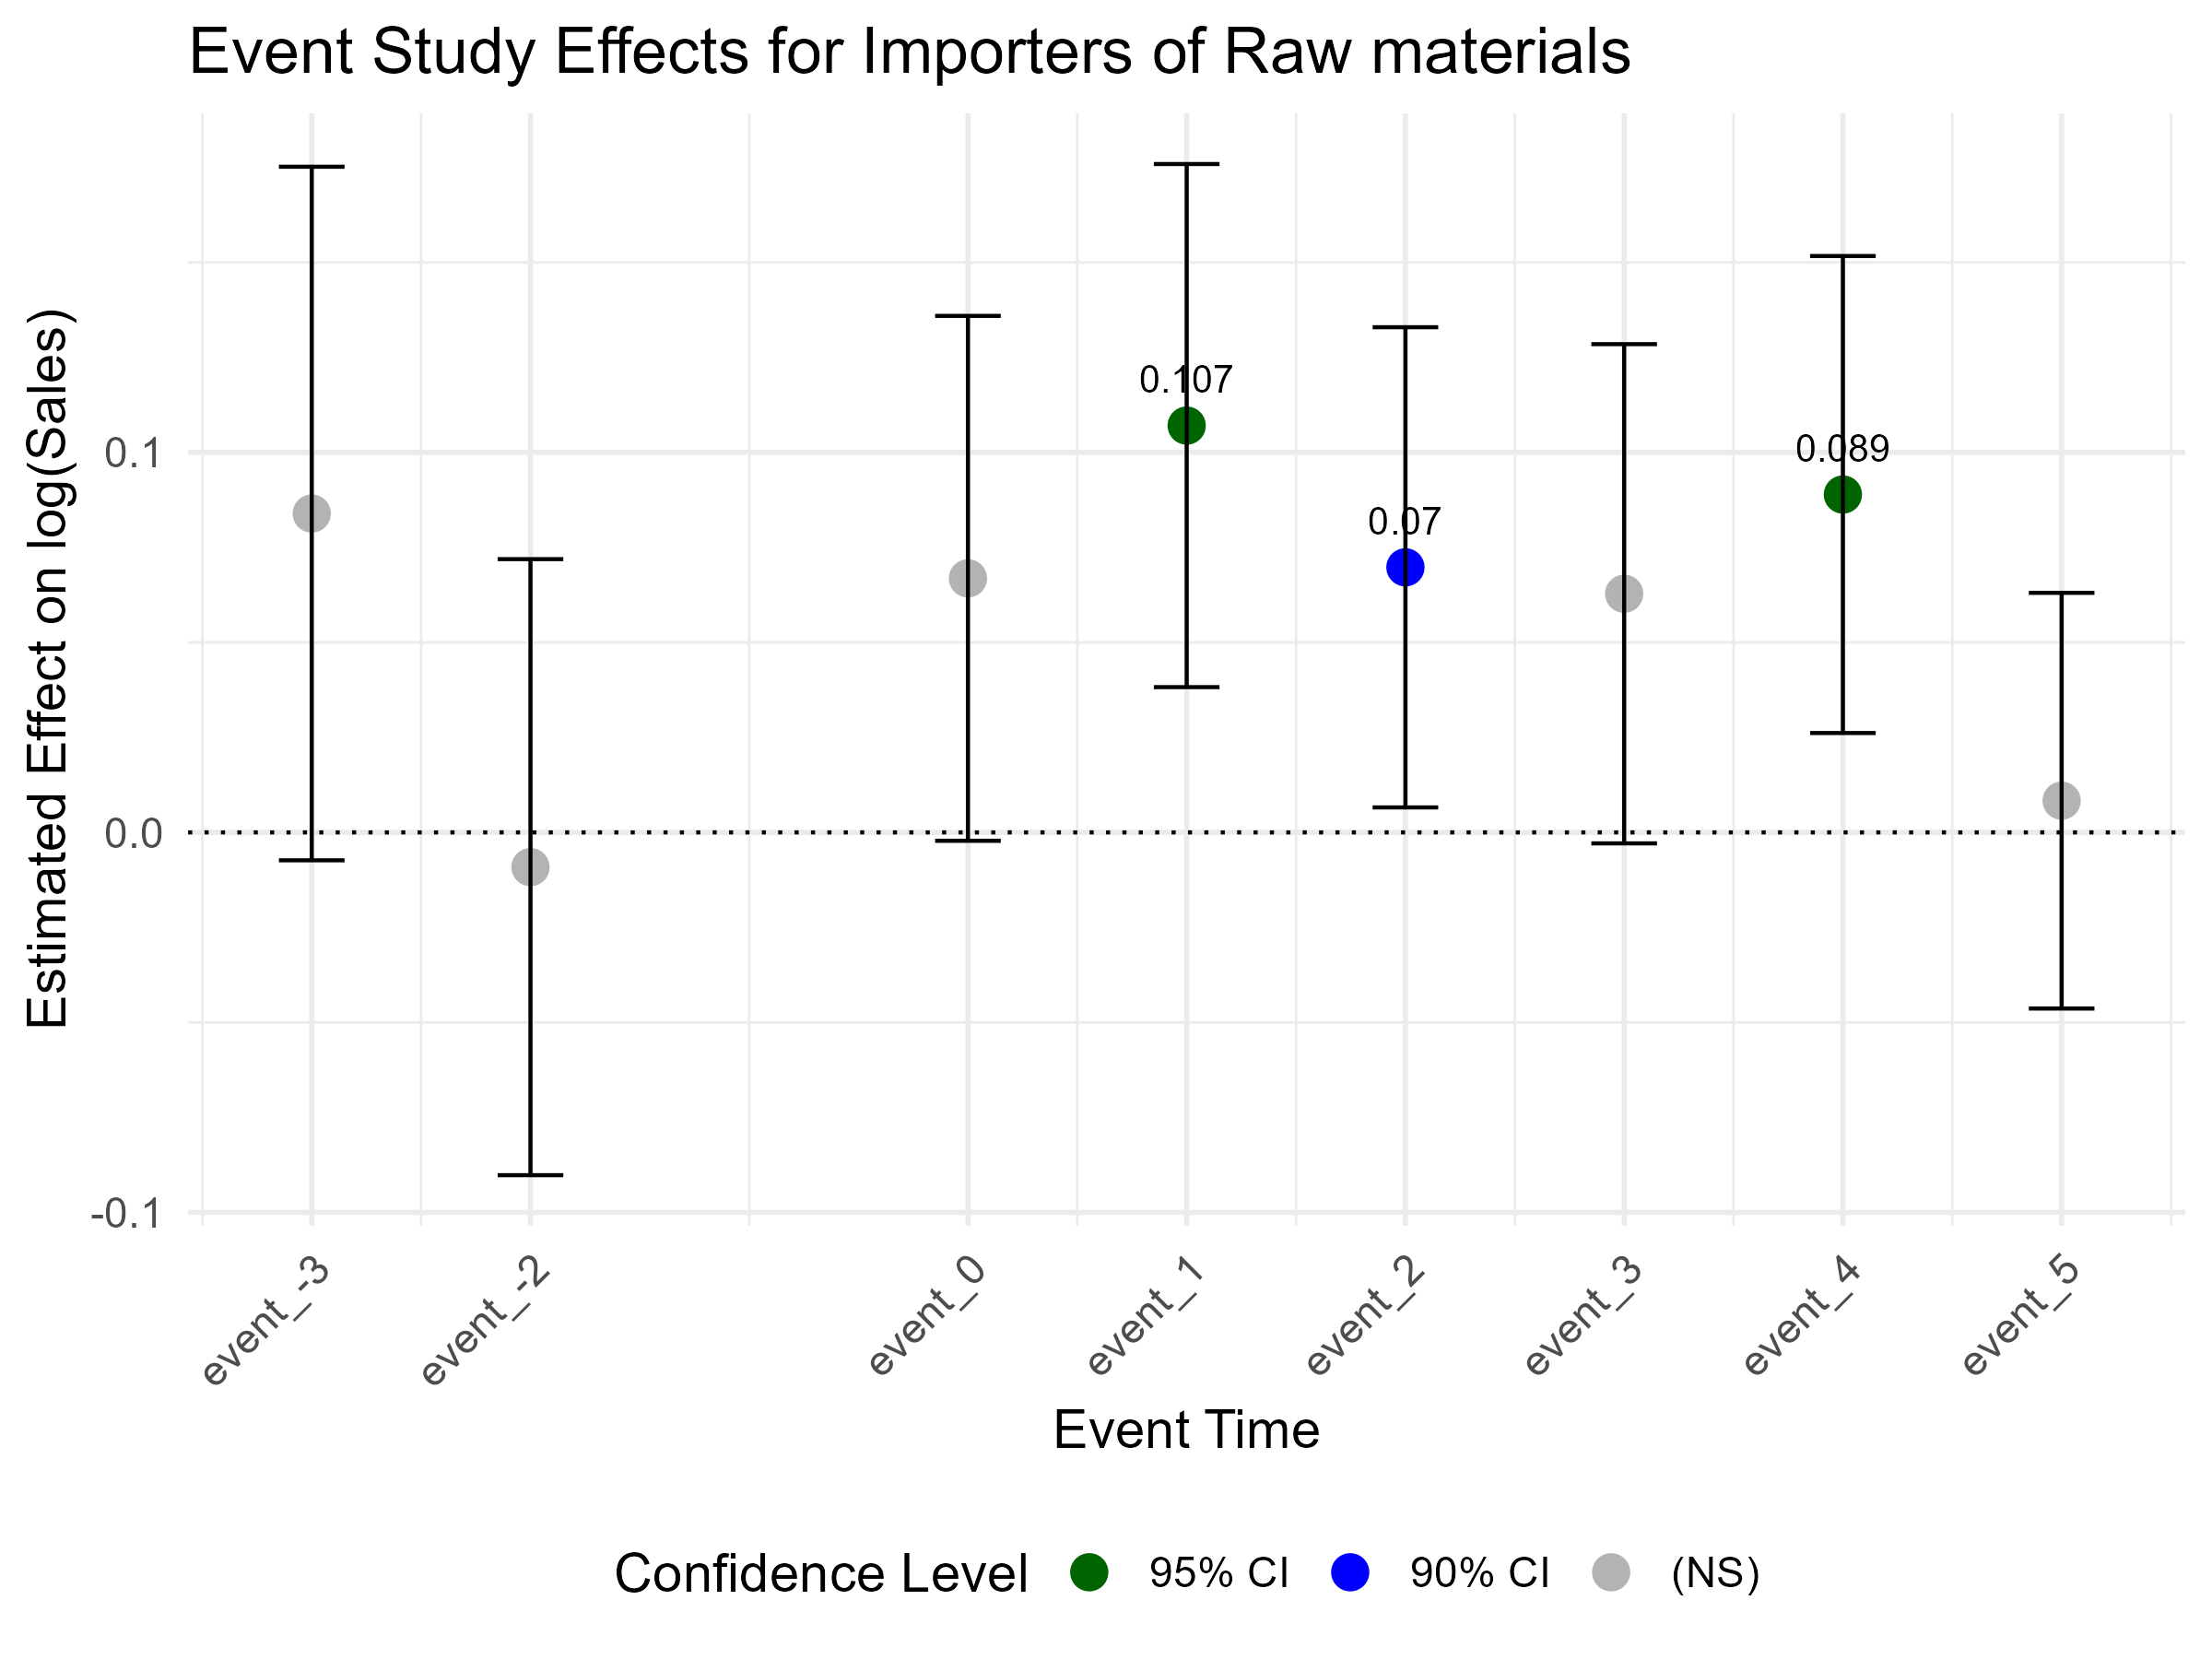
\includegraphics[width=\linewidth]{Imp_raw.png}
                    \caption{Raw materials importers}
                    \label{fig:Impraw}
                \end{subfigure}
                \hfill
                \begin{subfigure}[t]{0.45\textwidth}
                    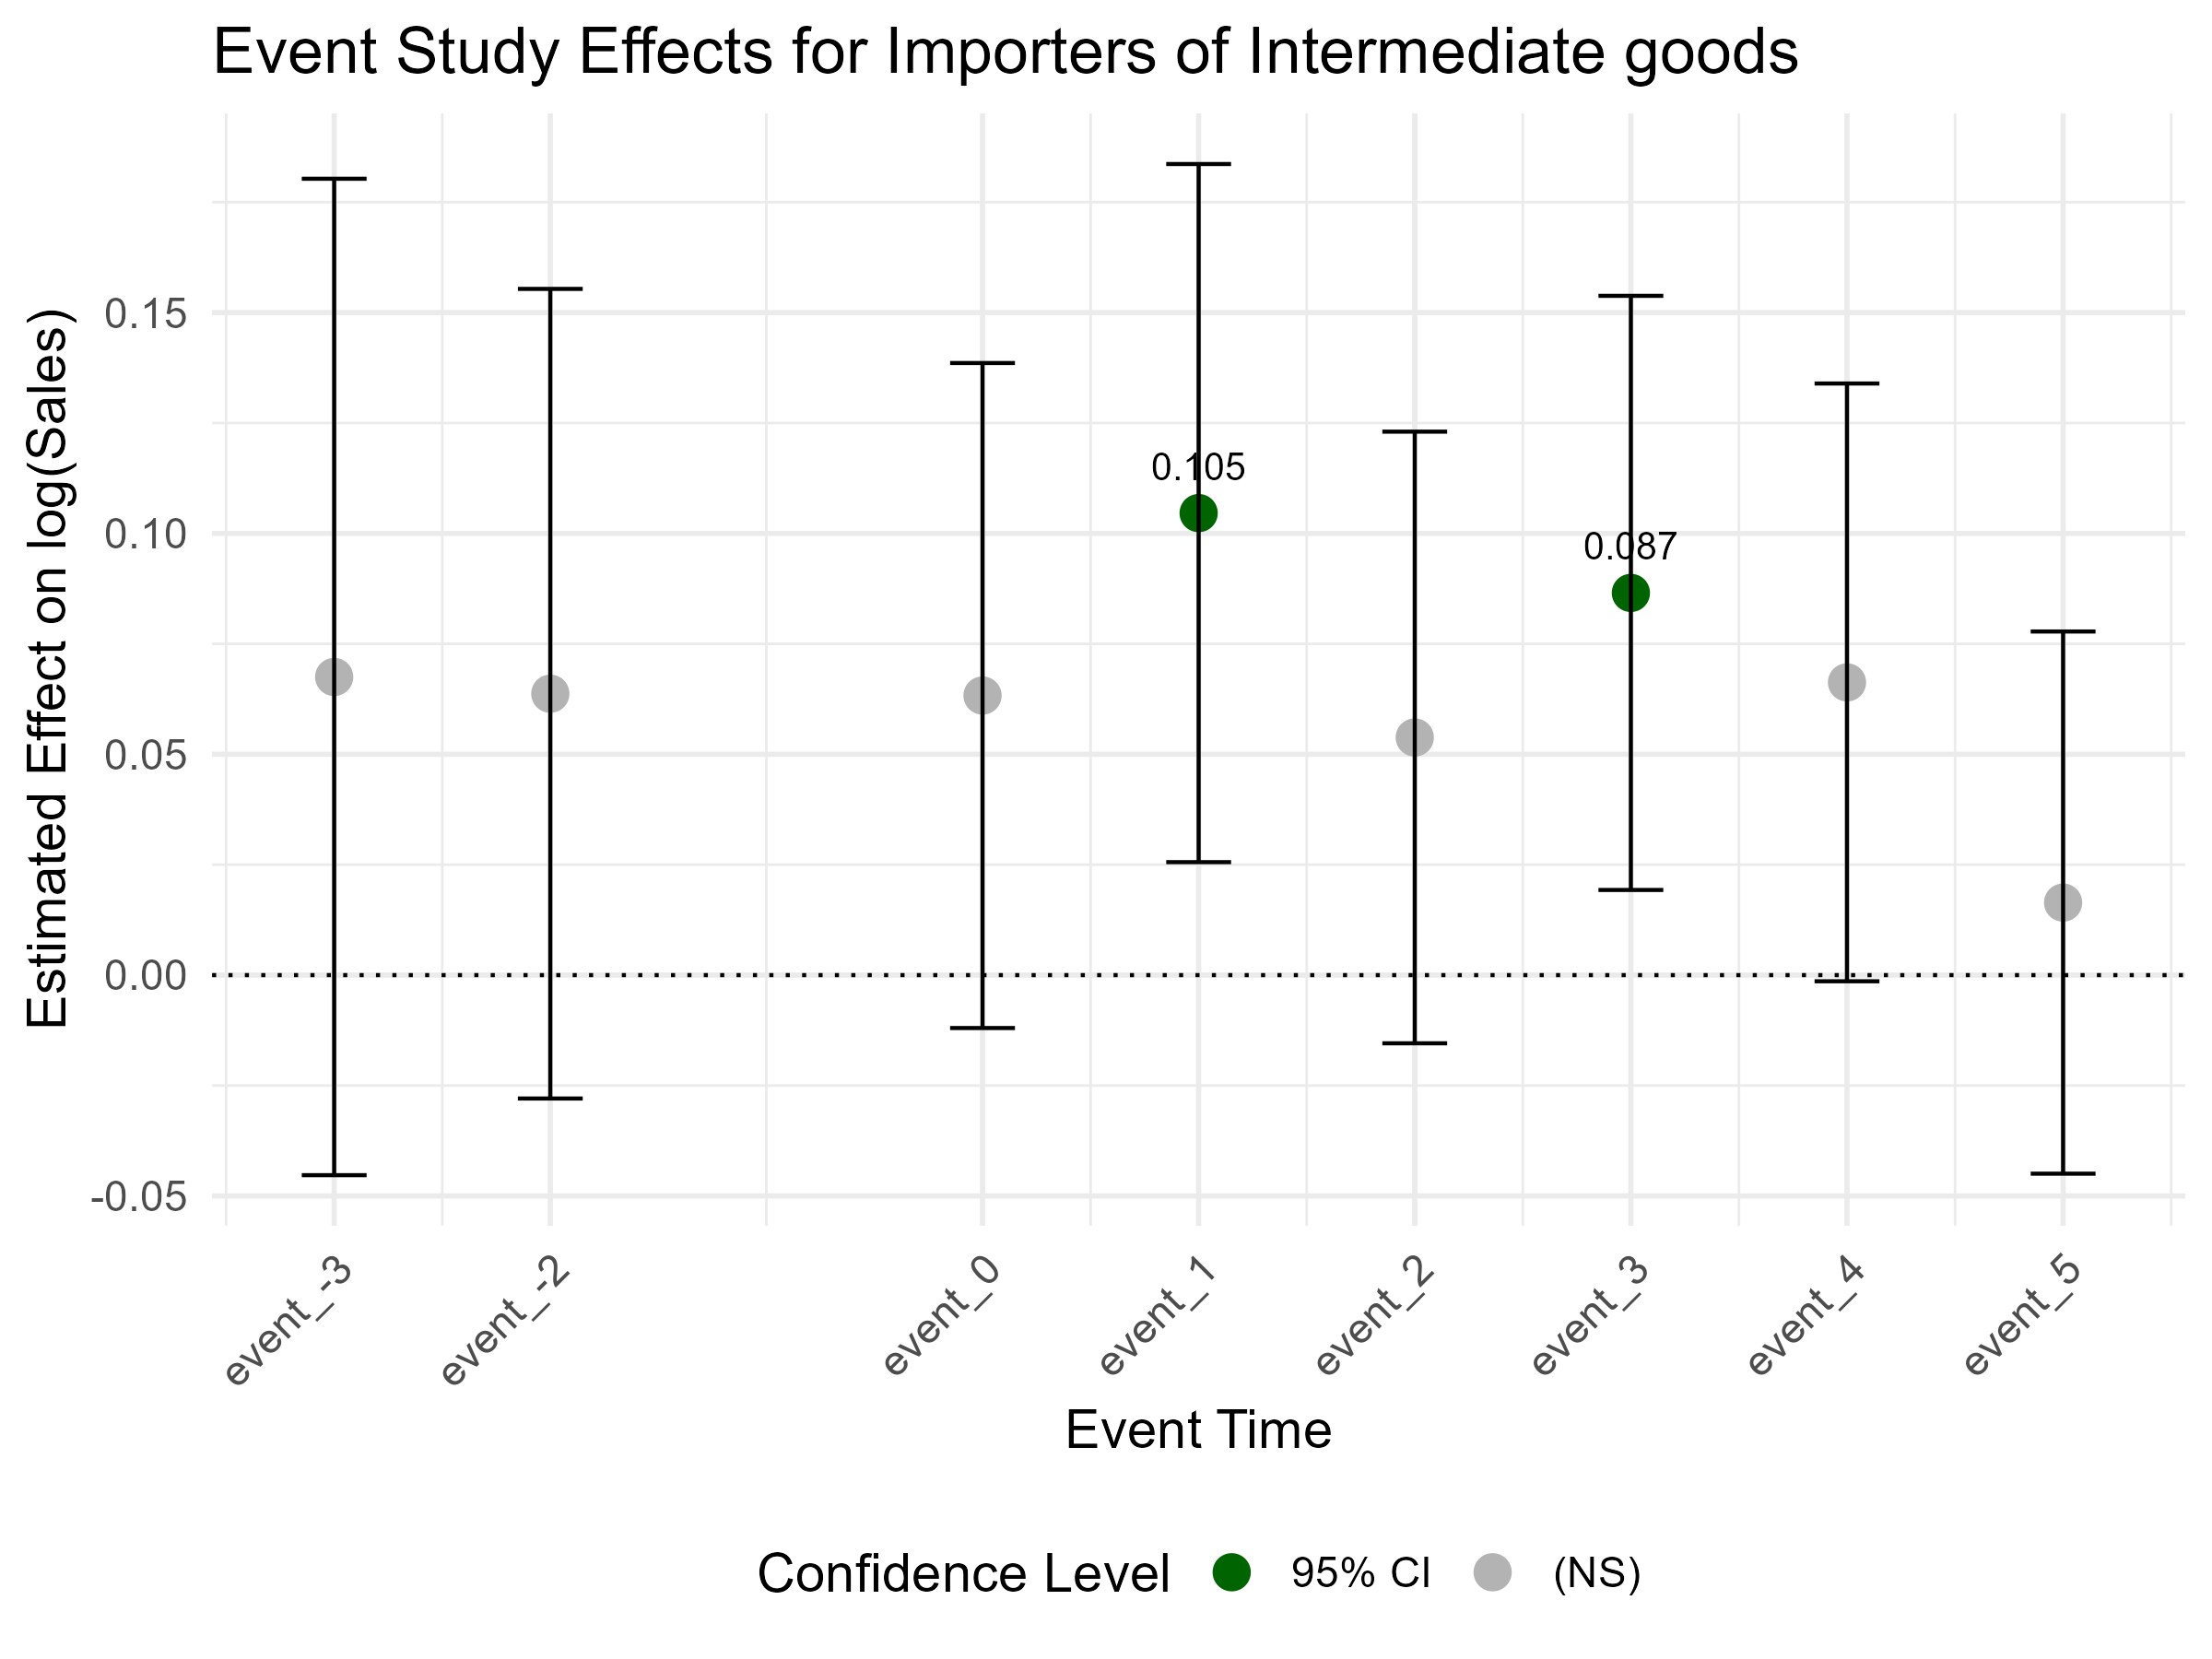
\includegraphics[width=\linewidth]{Imp_int.png}
                    \caption{Intermediate goods importers}
                    \label{fig:Impint}
                \end{subfigure}
                
                \vspace{0.4cm}
                
                \begin{subfigure}[t]{0.45\textwidth}
                    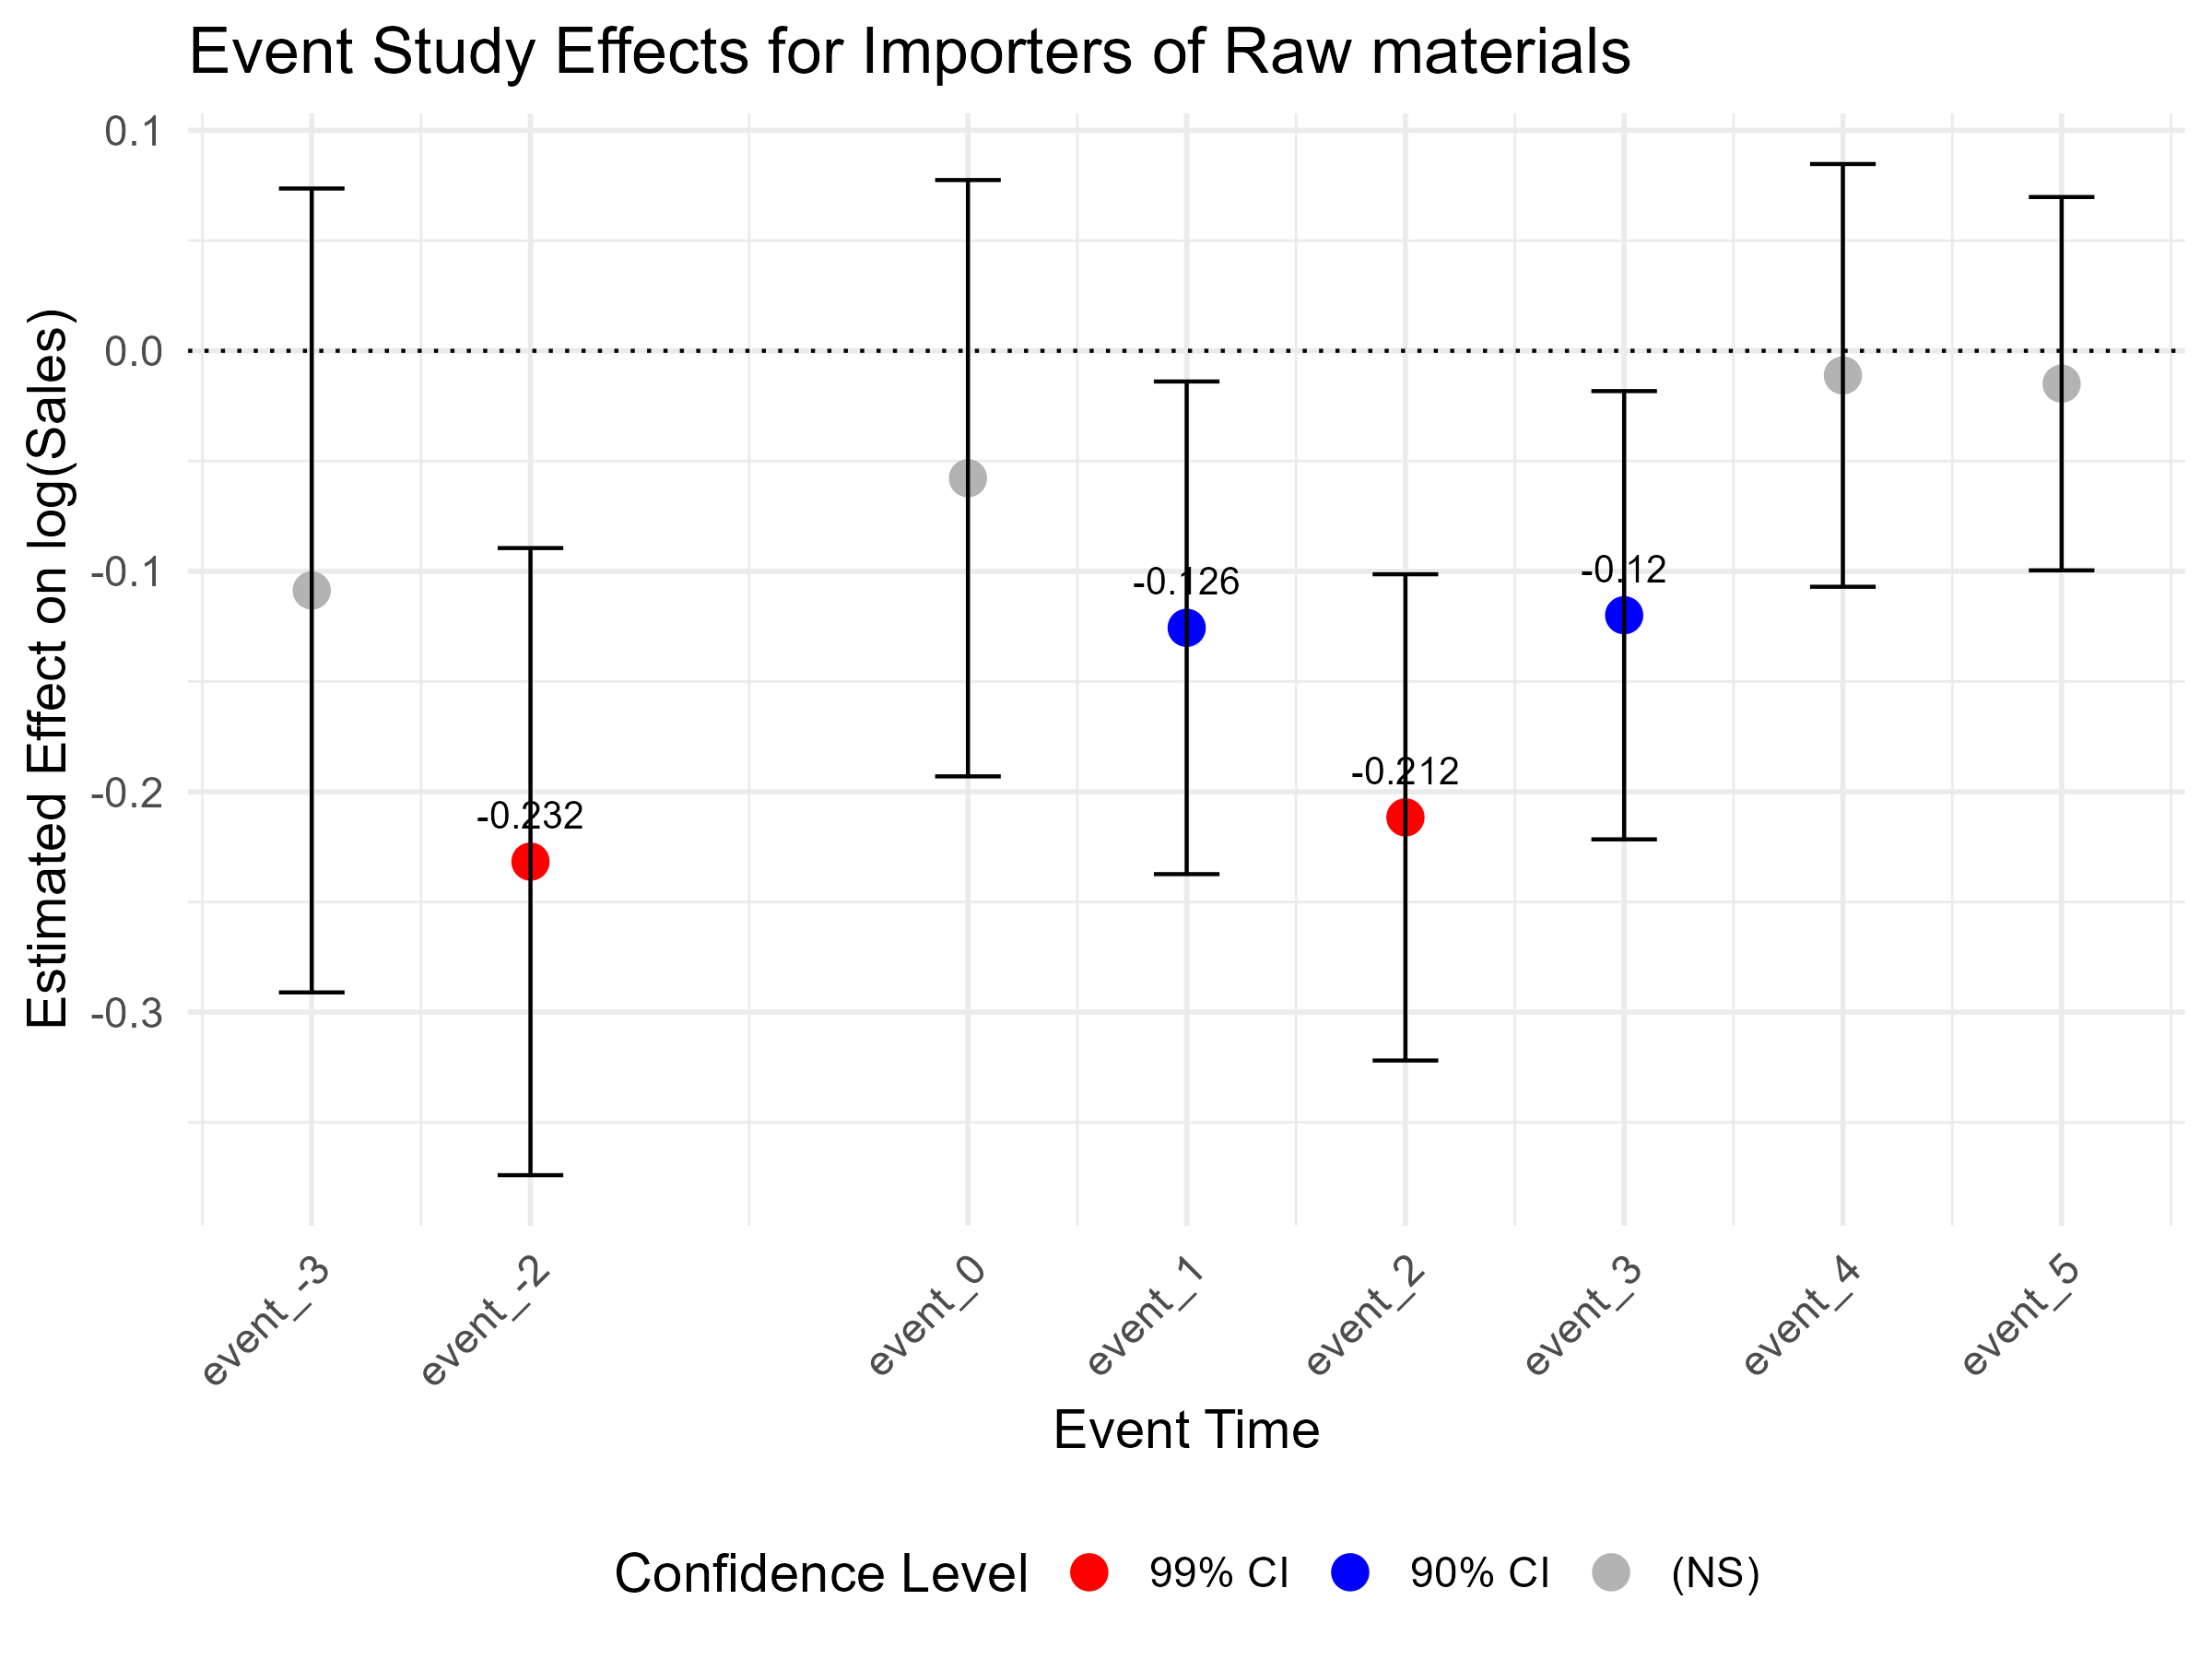
\includegraphics[width=\linewidth]{Imp_fin.png}
                    \caption{Finished goods importers}
                    \label{fig:Impfin}
                \end{subfigure}
                \hfill
                \begin{subfigure}[t]{0.45\textwidth}
                    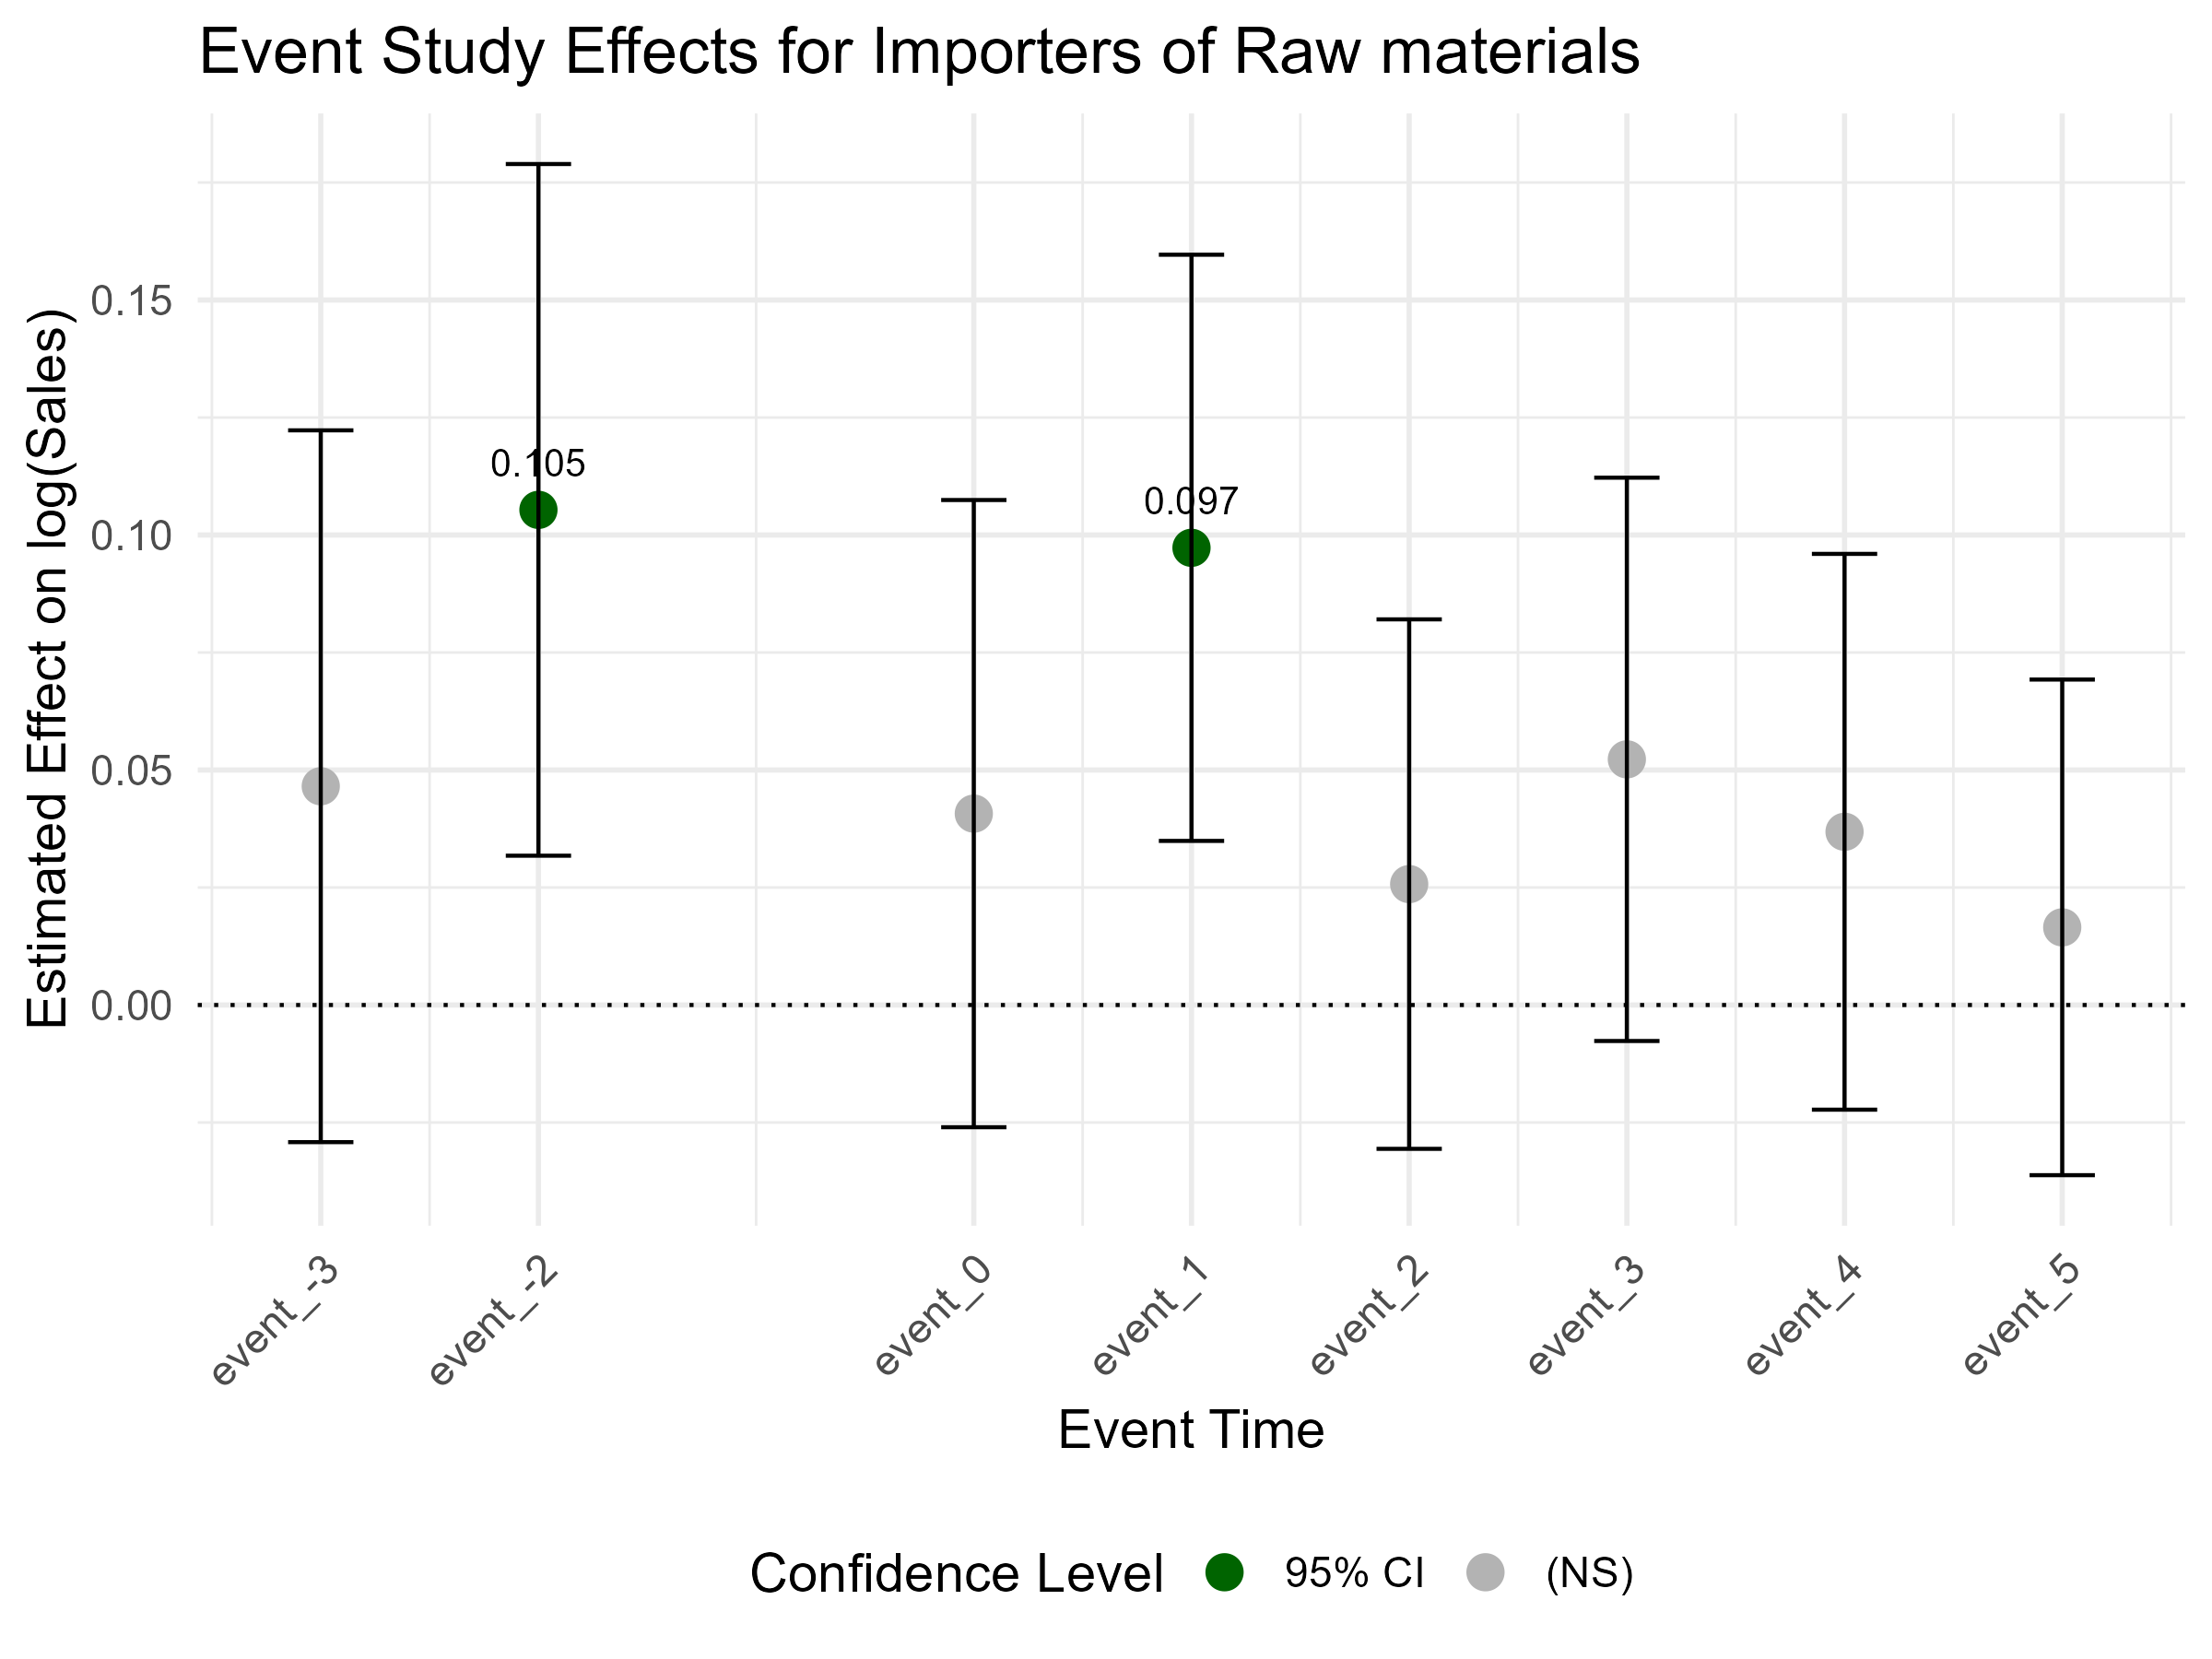
\includegraphics[width=\linewidth]{Imp_cap.png}
                    \caption{Capital importers}
                    \label{fig:Impcap}
                \end{subfigure}
            \end{minipage}
        };
        
        % Vertical line between columns
        \draw[line width=0.4pt] (0,6.5) -- (0,-6.5);
        
        % Horizontal line between rows
        \draw[line width=0.4pt] (-9, 0) -- (9, 0);
    \end{tikzpicture}
    \vspace{0.25cm}
    \caption{Impact of Extreme Natural Disasters on Different Types of Importers}
    \label{fig:import_panel_with_lines}
\end{figure}

Columns 1-4 of Table \ref{tab:main_interactions} highlight the magnitude of these impacts. Firms that import raw materials and intermediate goods are better off other firms when a disaster occur (columns 1 \& 2). Indeed, the sales of these firms increase by 6\%  on average compared to other companies affected by natural disasters. Their sales continue to increase by 10.5\% on average in $\text{t}_{+1}$, and 6\% in $\text{t}_{+2}$. In the medium term, their sales are still increasing compared to other affected firms by on average 7\% in $\text{t}_{+4}$ and $\text{t}_{+5}$.
Compared to their siblings in unaffected regions, importers of raw material and intermediate goods still increase their sales. However, the magnitude is less important compared to other firms affected by the disaster. Indeed, they increase their sales on average 3\% in the year of the event.

\newpage
In the short term ($\text{t}_{+1}$, $\text{t}_{+2}$), their sales increase by 4\% and 6\% on average\footnote{These coefficients are the difference between the interaction coefficient in table \ref{tab:main_interactions} and the baseline coefficient in table \ref{tab:main_interactions_baseline} in appendices}. In the medium term ($\text{t}_{+3}$, $\text{t}_{+4}$), this increase stabilizes around 5\% on average.

\begin{table}[H]\centering
\caption{Event Study: Differential Impact on Importers Sales}
\label{tab:main_interactions}
\begin{tabular}{lccccc}
\toprule
 & Raw Materials & Intermediate & Finished & Capital & All Importers \\
\textit{Estimation Results} & (1) & (2) & (3) & (4) & (5) \\
\midrule
\multicolumn{6}{l}{\textit{Immediate Effect}} \\
event\_0 & 0.0669$^{***}$ & 0.0633$^{*}$ & -0.0578$^{*}$ & 0.0407         & 0.0569$^{.}$ \\
                    & (0.0094)       & (0.0311)     & (0.0237)       & (0.0327)       & (0.0309)     \\
\midrule
\multicolumn{6}{l}{\textit{Short-Term Effect}} \\
event\_1 & 0.1071$^{***}$ & 0.1046$^{***}$ & -0.1256$^{***}$ & 0.0973$^{***}$ & 0.1058$^{***}$ \\
                    & (0.0176)       & (0.0191)       & (0.0309)        & (0.0214)       & (0.0214)     \\
event\_2 & 0.0698$^{***}$ & 0.0538$^{**}$  & -0.2116$^{***}$ & 0.0257         & 0.0501$^{*}$ \\
                    & (0.0108)       & (0.0170)       & (0.0562)        & (0.0271)       & (0.0219)     \\
\midrule
\multicolumn{6}{l}{\textit{Medium/Long Term Effect}} \\
event\_3 & 0.0628$^{*}$   & 0.0865$^{***}$ & -0.1199$^{***}$ & 0.0523         & 0.0894$^{***}$ \\
                    & (0.0261)       & (0.0114)       & (0.0195)        & (0.0353)       & (0.0086)     \\
event\_4 & 0.0889$^{***}$ & 0.0663$^{***}$ & -0.0112         & 0.0369$^{*}$   & 0.0700$^{***}$ \\
                    & (0.0206)       & (0.0110)       & (0.0303)        & (0.0185)       & (0.0126)     \\
event\_5 & 0.0083         & 0.0164         & -0.0149         & 0.0165         & 0.0214       \\
                    & (0.0224)       & (0.0402)       & (0.0093)        & (0.0415)       & (0.0410)     \\
\midrule
\multicolumn{6}{l}{\textit{Controls}} \\
Productivity (tfp\_lp)            & 0.7032$^{***}$ & 0.7007$^{***}$ & 0.7030$^{***}$ & 0.7022$^{***}$ & 0.7017$^{***}$ \\
                   & (0.0363)       & (0.0378)       & (0.0368)       & (0.0375)       & (0.0363)       \\
Log electricity       & 0.6748$^{***}$ & 0.6727$^{***}$ & 0.6745$^{***}$ & 0.6752$^{***}$ & 0.6736$^{***}$ \\
                   & (0.0154)       & (0.0185)       & (0.0162)       & (0.0160)       & (0.0154)       \\
Log asset             & 0.0003         & 0.0002         & 0.0003         & 0.0003         & 0.0003         \\
                   & (0.0003)       & (0.0004)       & (0.0003)       & (0.0003)       & (0.0003)       \\
Log leverage          & 0.0159         & 0.0157         & 0.0160         & 0.0158         & 0.0159         \\
                   & (0.0108)       & (0.0110)       & (0.0110)       & (0.0111)       & (0.0109)       \\
\midrule
Observations       & 8,830          & 8,830          & 8,830          & 8,830          & 8,830          \\
R$^2$              & 0.9654         & 0.9655         & 0.9648         & 0.9654         & 0.9655         \\
Within R$^2$       & 0.6045         & 0.6061         & 0.5975         & 0.6047         & 0.6058         \\
Fixed Effects      & \multicolumn{5}{c}{Firm and Industry-Year and Group-Year} \\
Standard Errors    & \multicolumn{5}{c}{Conley (690 km)} \\
\bottomrule
\end{tabular}
\begin{tablenotes}
\small
\item \textit{Note:} This table presents the interaction effects between event timing and importer type, as well as the main controls. Significance levels: $^{.}p<0.1$, $^{*}p<0.05$, $^{**}p<0.01$, $^{***}p<0.001$.
Columns 1-5 represents the estimated coefficients of the differential impact of natural disasters on treated firms in each
sourcing type, relative to both (ii) treated firms in the baseline sector (Non importers affected by the disaster).Conley-adjusted standard errors (in parentheses). Control variables include: TFP, leverage, electricity use, total assets, cumulative droughts, floods, and cyclones.
Comparison with (ii) non-treated firms in the same sourcing type can be done with the main coefficients in Table \ref{tab:main_interactions_baseline}. *** $p < 0.001$, ** $p < 0.01$, * $p < 0.05$, . $p < 0.1$.
\end{tablenotes}
\end{table}

Interestingly, finished goods importers do not share the same fate. Column 3 shows that these firms saw their sales decrease in the short and medium term compared to other affected firms. This loss spiked to 20\% two years after the disaster. This fuels the theory that the import of inputs, such as raw or intermediate goods, is the driver of resilience against extreme disasters. Companies that import capital (column 4) follow a trend similar to input importers, but the magnitude of their sales increase is lower and does not hold in the medium term. 

\section{Mechanisms \& Robustness}

\subsection{\textit{Alternative Outcomes}}

\subsubsection{Wages}

Along with a drop in their companies' sales, workers in Primary \& Processed products industries saw their wages drop in the year following the disaster, as we can see in Figure \ref{fig:WagesPrim}. This drop was approximately of 15.6\% compared to workers in the chemical and mineral industries and 10\% compared to workers in Primary \& Processed products in states not affected by disasters (Table \ref{tab:event_sector_interaction_wages}). However, the firms were able to recover in the following period, leading to no significant differences in wages in the next periods. \\

Workers in light manufacturing firms also shared a loss in wages. This loss was on average about 27.7\% in the year of the disaster and about 30.7\% in the following year compared to the baseline industry (Figure \ref{fig:WagesManuf}). Compared to non-affected light manufacturing workers, this effect is slightly lower (22\%) but still significant (Table \ref{tab:event_sector_interaction_wages}).

\begin{figure}[H]
    \centering
    \begin{subfigure}[t]{0.48\textwidth}
        \centering
        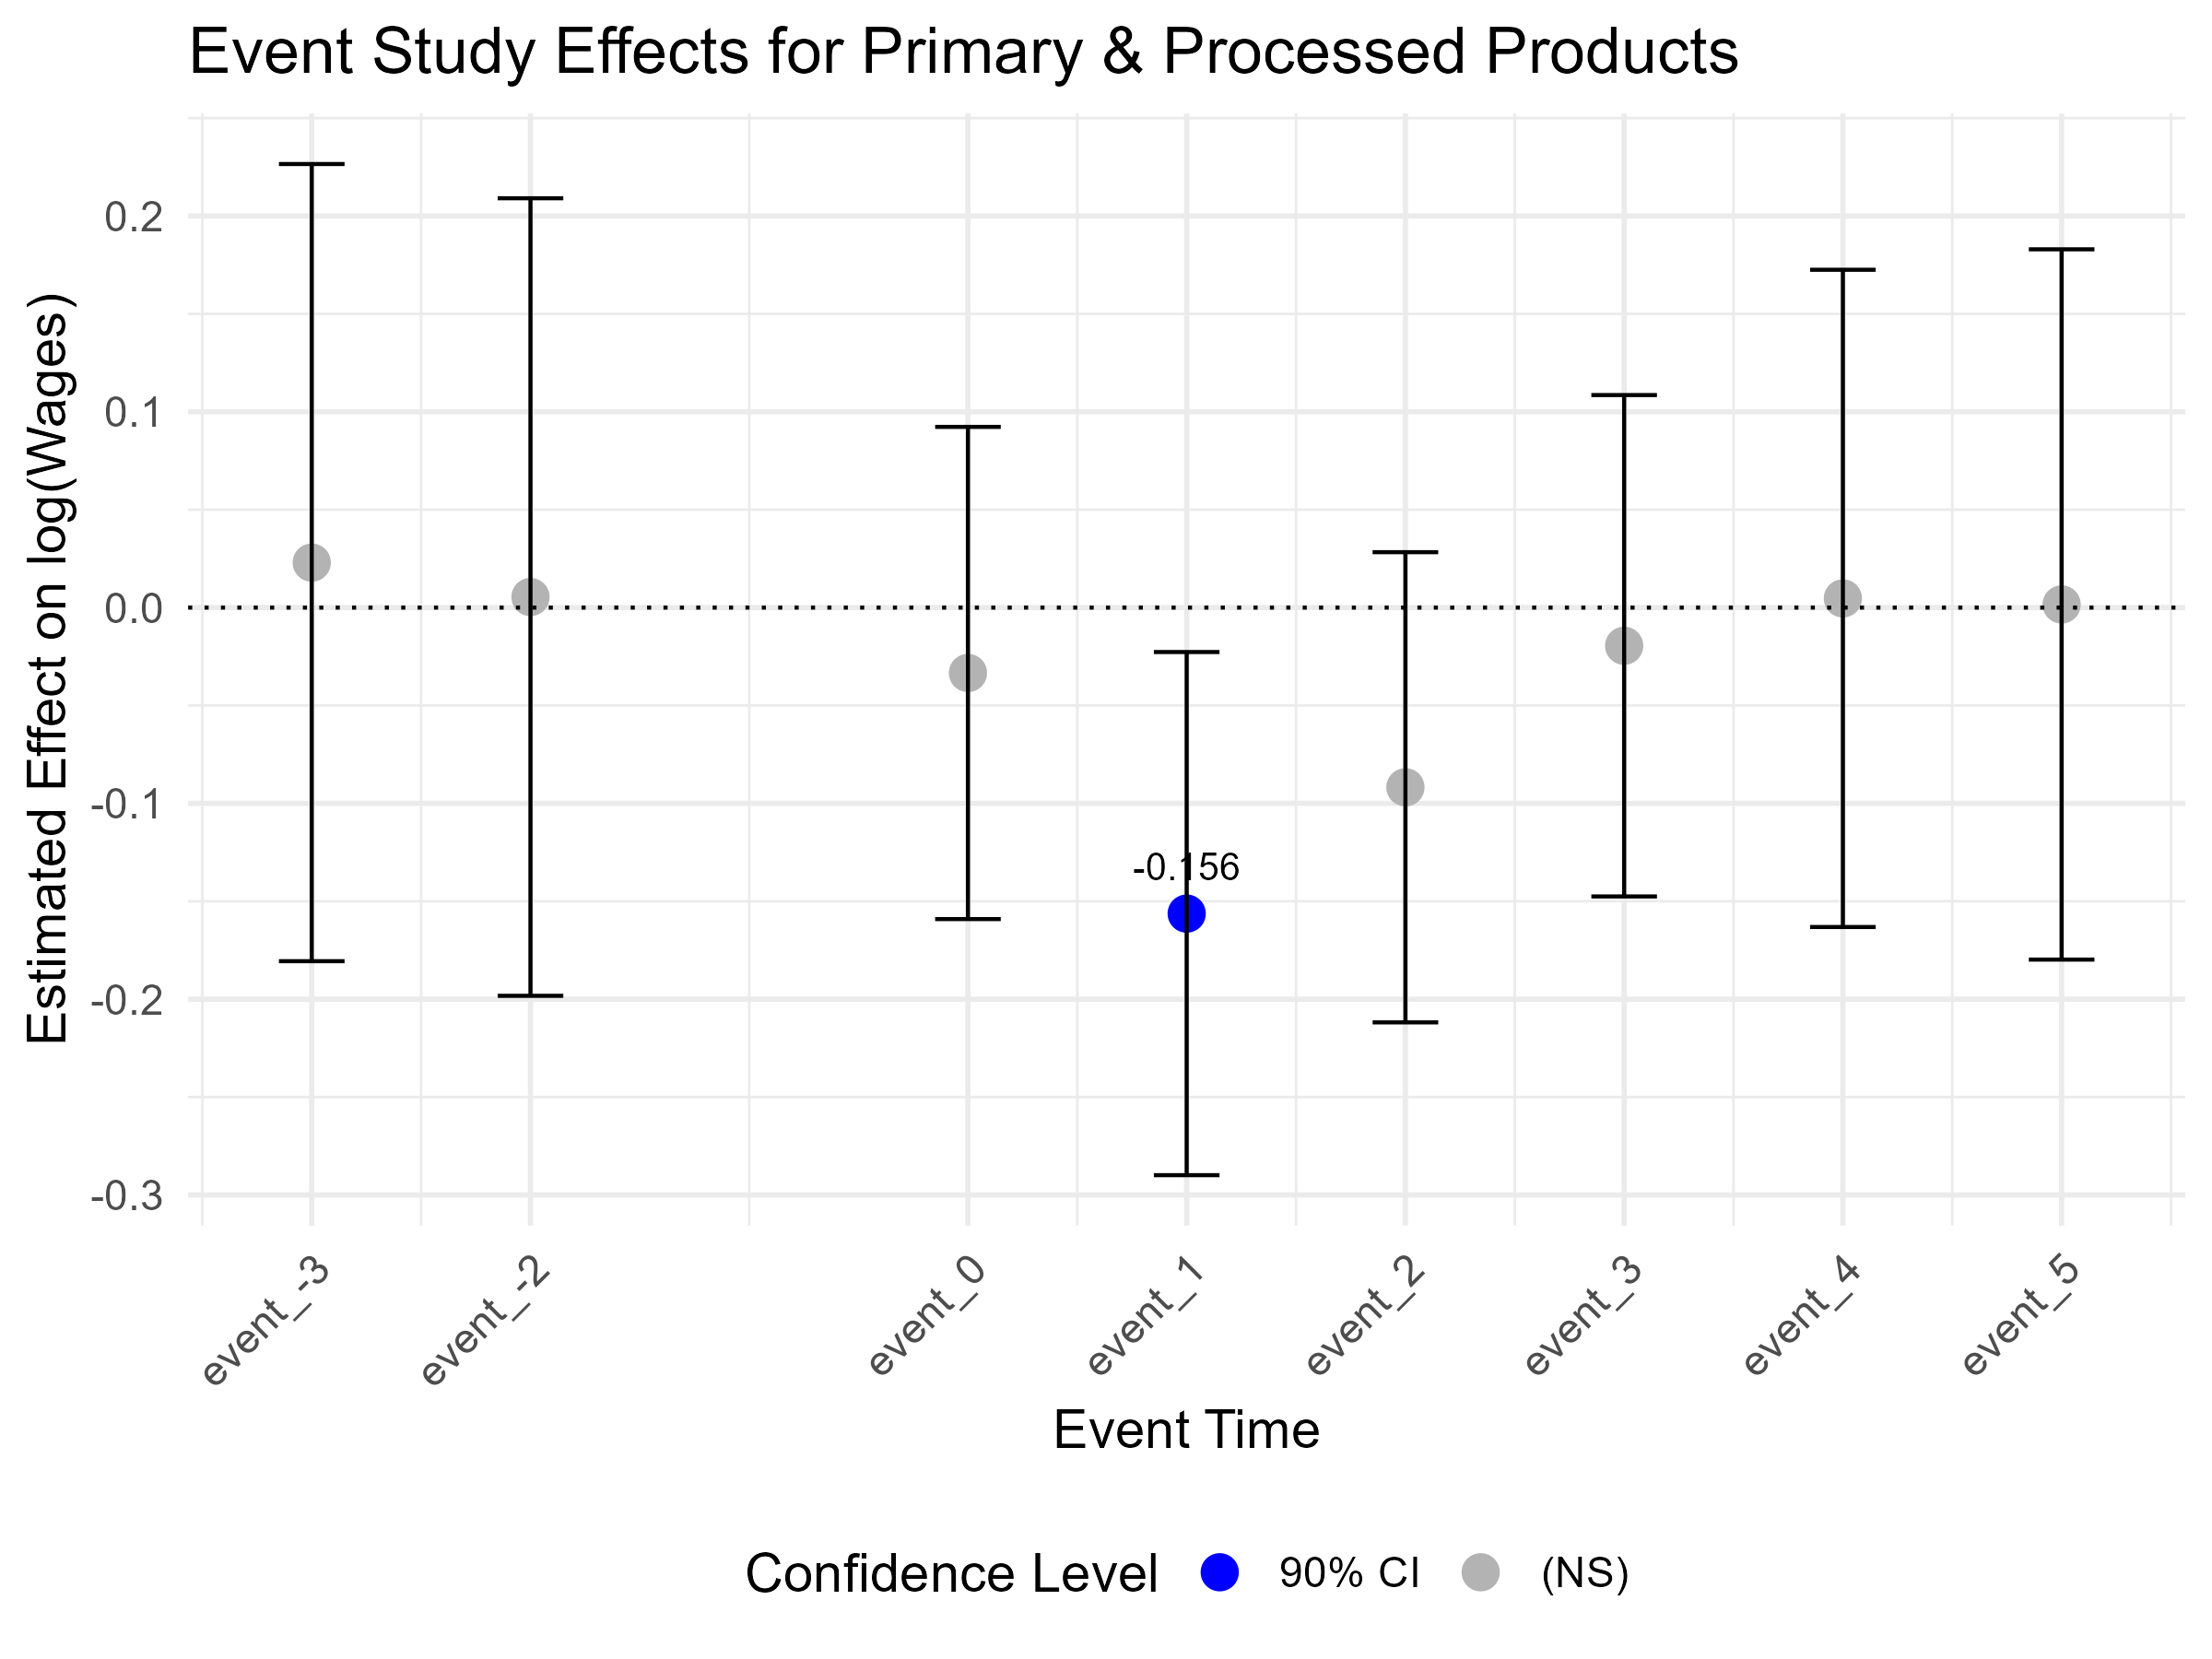
\includegraphics[width=\linewidth]{PrimIndustries wages.png}
        \caption{Primary \& Processed firms}
        \label{fig:WagesPrim}
    \end{subfigure}%
    \hfill
    \begin{subfigure}[t]{0.48\textwidth}
        \centering
        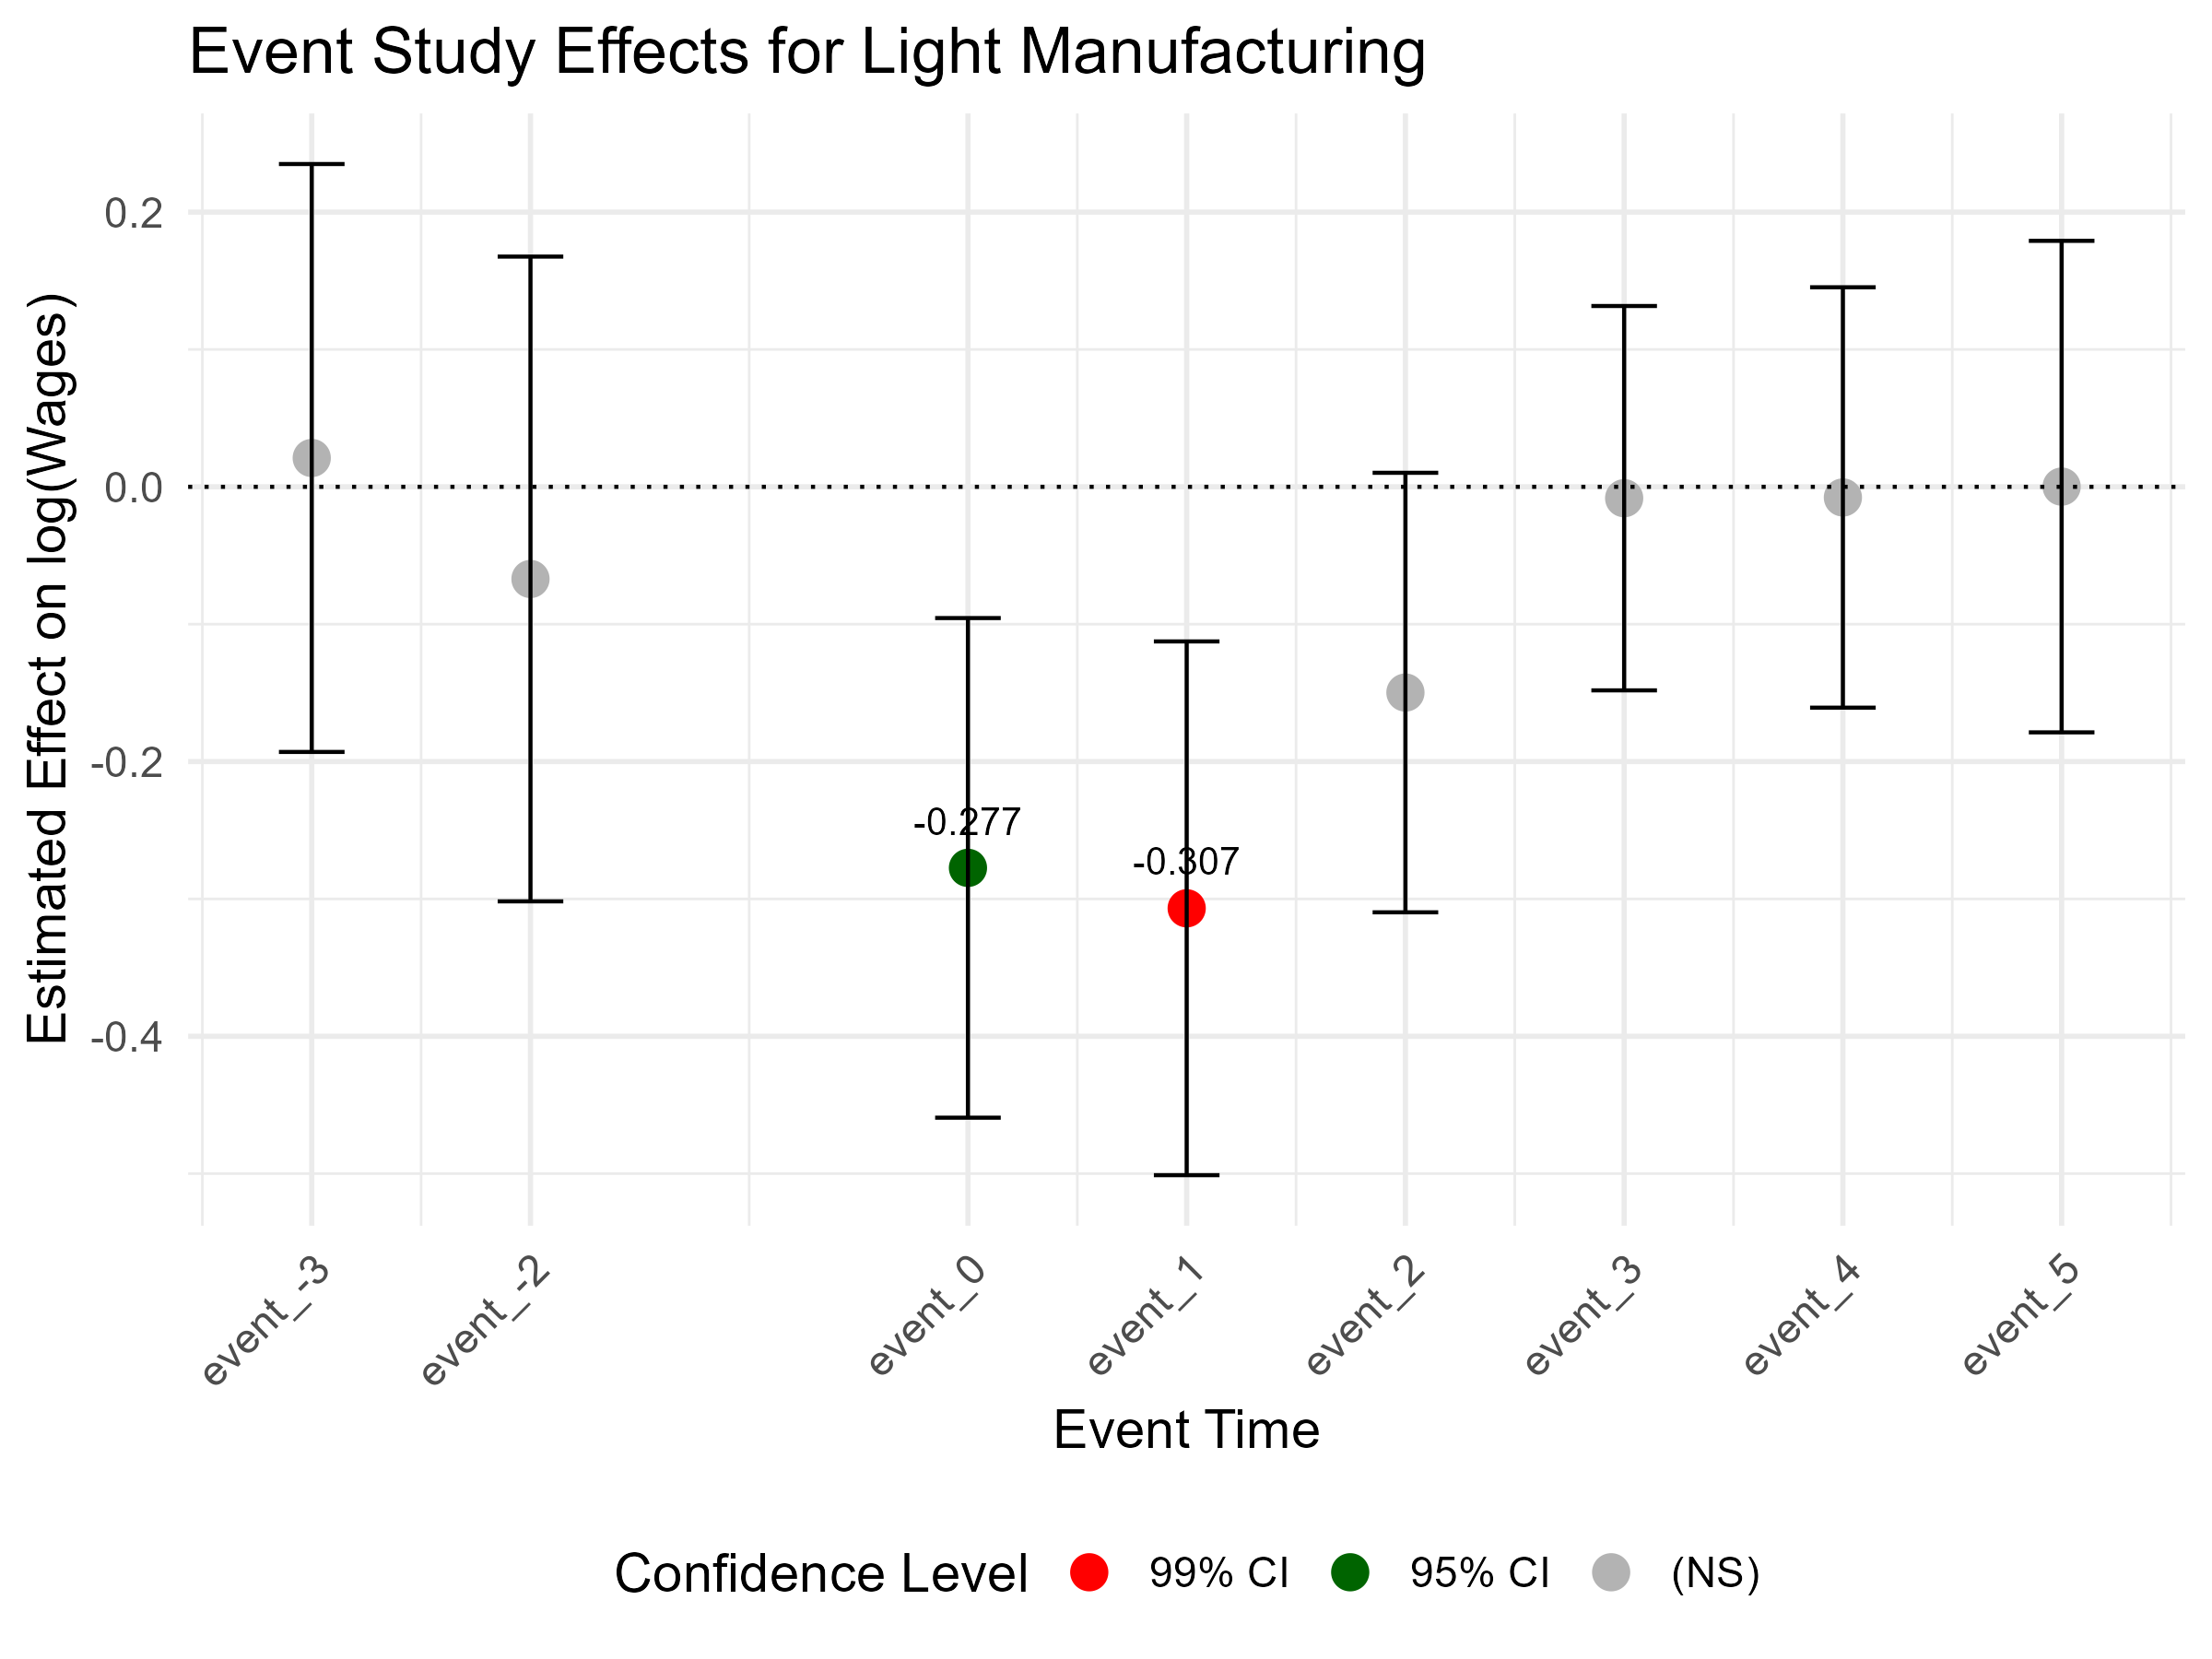
\includegraphics[width=\linewidth]{Light Manufacturing wages.png}
        \caption{Light Manufacturing firms}
        \label{fig:WagesManuf}
    \end{subfigure}
    \caption{Impact of Extreme Natural Disasters on Firm Wages by Sector}
    \label{fig:WagesBySector}
\end{figure}

Firms in machinery and capital goods industries also observed their wages drop due to natural disasters compared to firms in chemical and minerals industries affected. The wages are on average 9\% lower in $\text{t}_{+1}$ and 4\% in $\text{t}_{+2}$. However, this loss in wages is not significant if we compare it with firms in machinery and capital goods not affected by disasters (column 4 of Table \ref{tab:event_sector_interaction_wages} of the Appendices).

\subsubsection{Productivity}

Due to damages caused by natural disasters, we could expect that firms lose in terms of productivity. Figure \ref{fig:ProdManuf} shows a decrease in productivity of approximately 15.1\% in $\text{t}_{+1}$ and 13.7\% in $\text{t}_{+2}$ compared to firms in the chemical and mineral industries. Firms recover three years after the event and productivity levels return to their trend levels before the disaster. Compared to non-affected firms in the light manufacturing industries, harmed ones lose on average 12\% of their productivity in the short term (column 3 of Table \ref{tab:event_sector_interaction_tfp}). In terms of magnitude, we are quite close to the findings of \cite{Bas2025}. They found that firms affected by the El-Nino rains in Ecuador saw their productivity drop by 11\% (TFP-Q) and 6.8\% (TFP-R).

\begin{figure}[H]
        \centering
        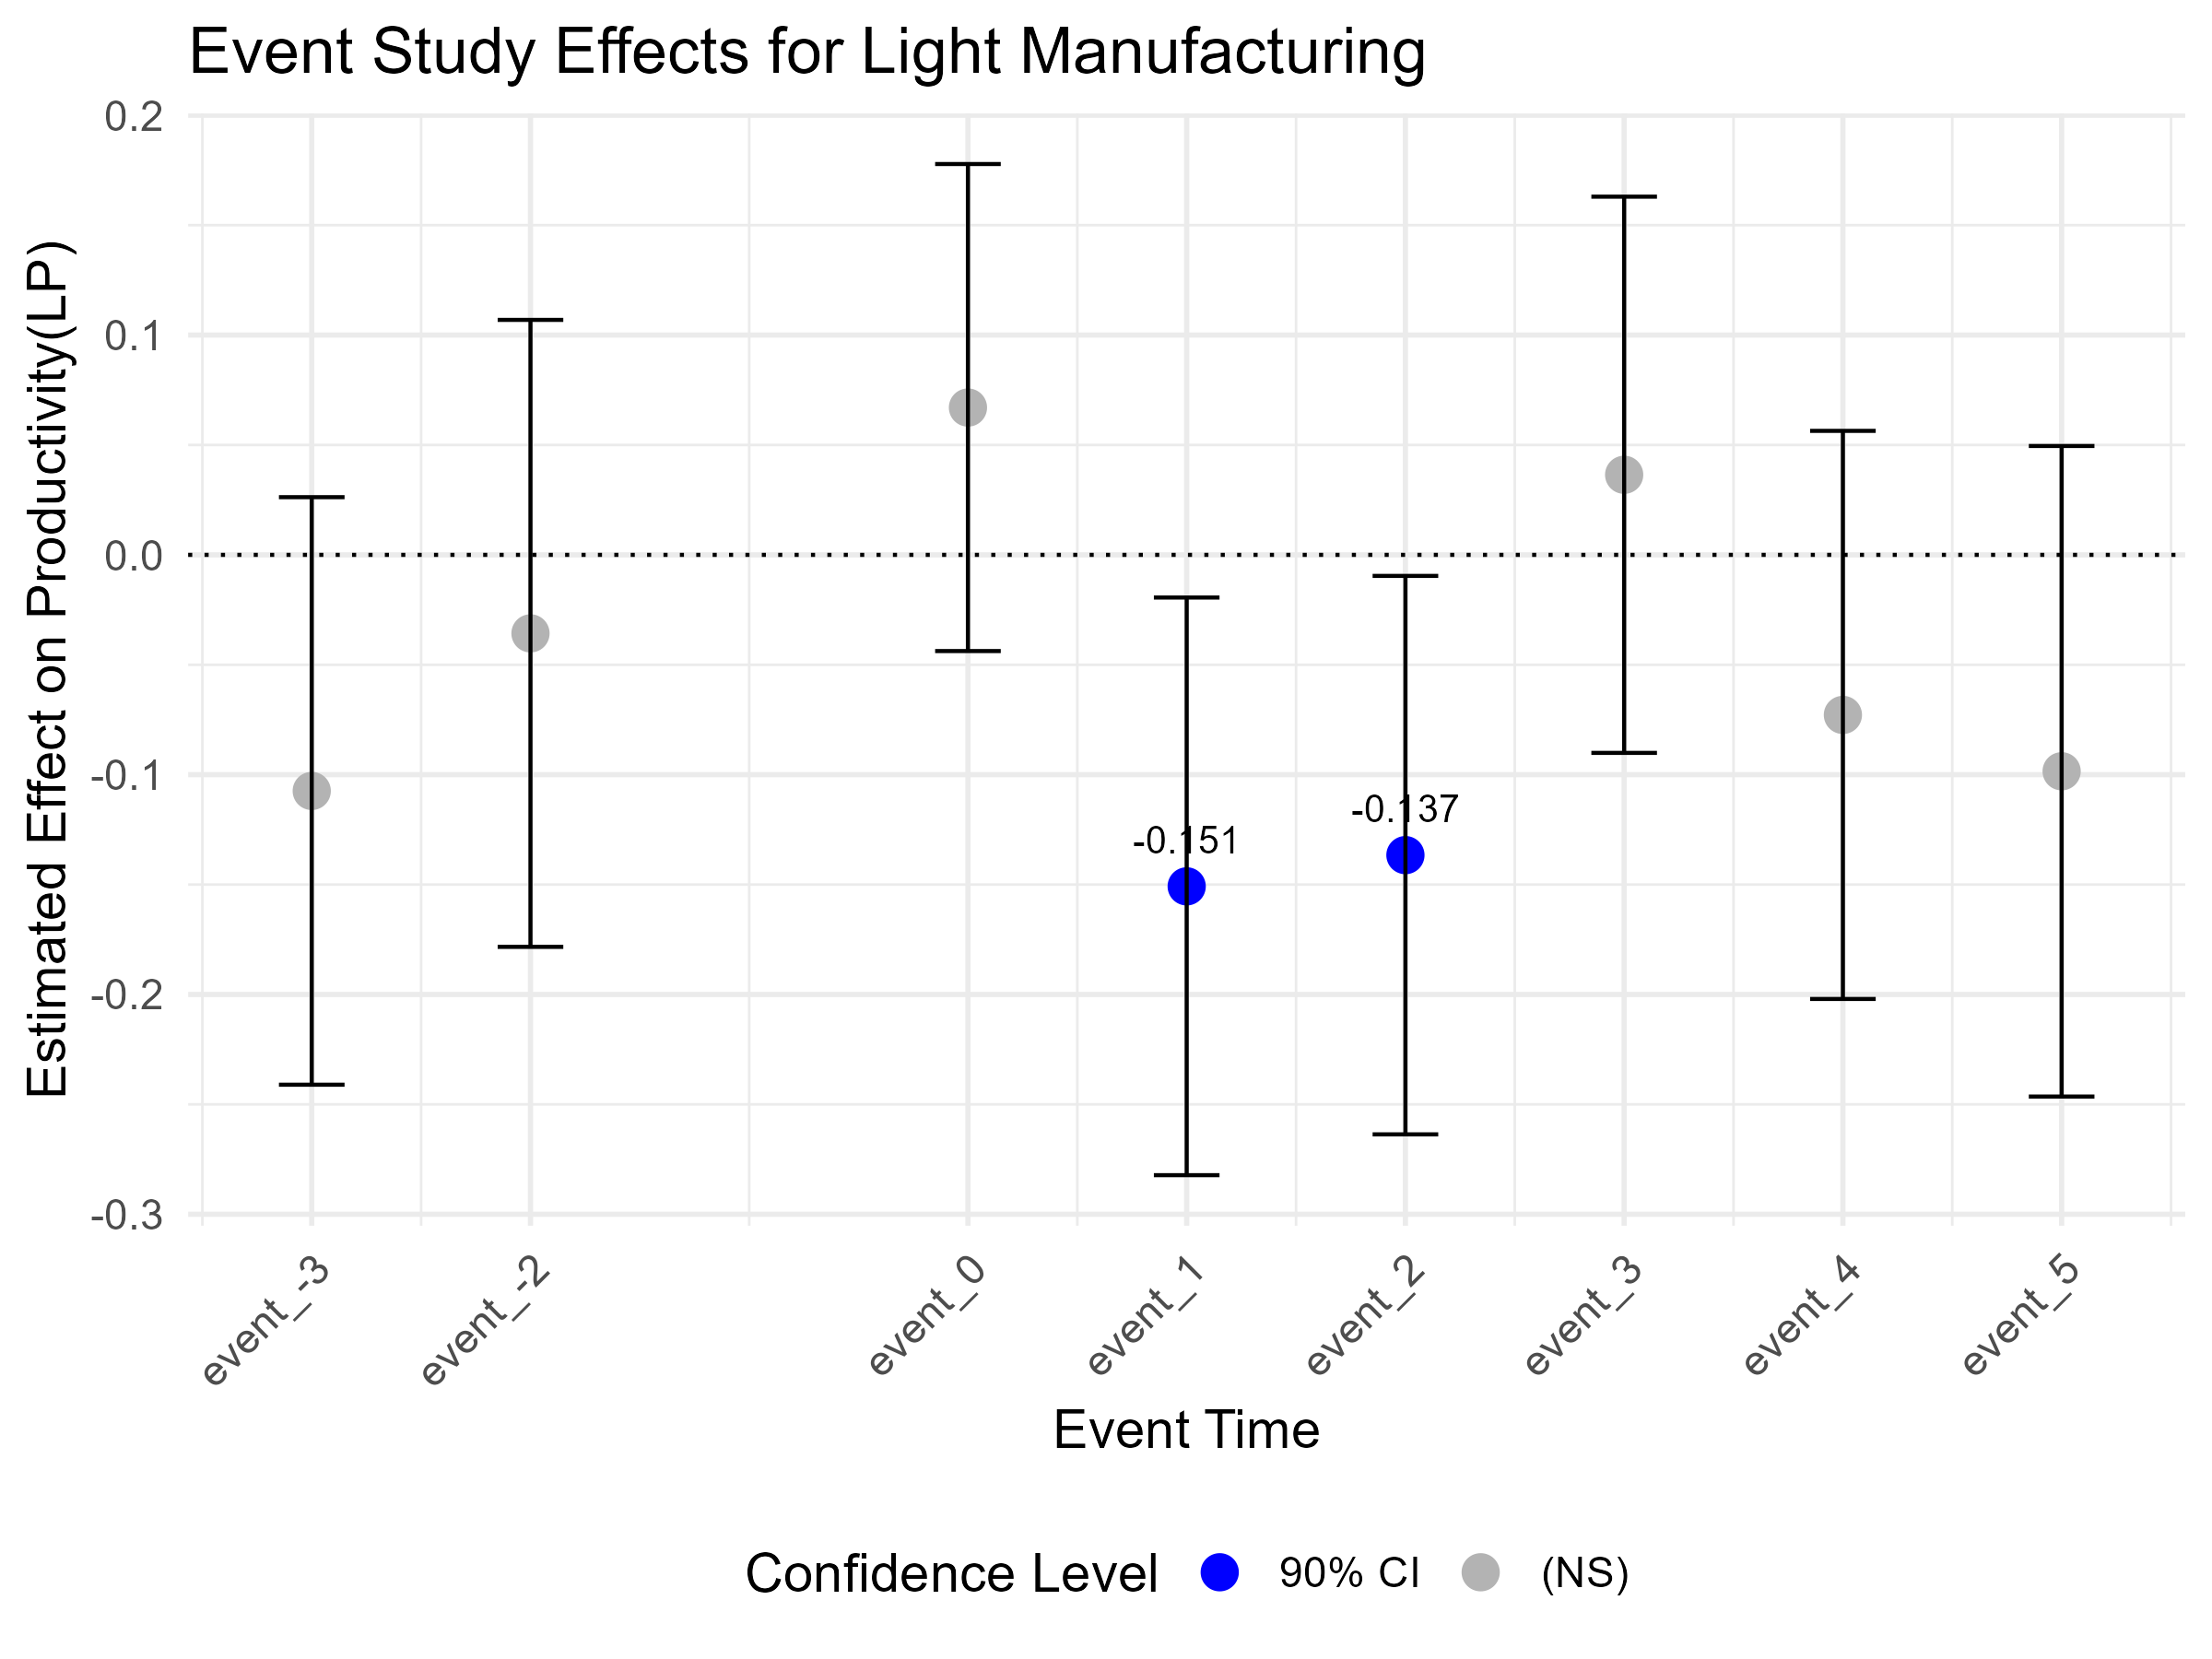
\includegraphics[width=0.55\linewidth]{Light_ManufacturingProd.png}
        \caption{Impact of Extreme Natural Disasters on productivity of Light Manufacturing firms}
        \label{fig:ProdManuf}
    \end{figure}

\subsubsection{Raw Materials}

Natural disasters disrupt supply chains, which, as we saw, ultimately leads to a decrease in sales for firms in Primary \& Processed products and Light Manufacturing industries. In this subsection, I provide an explanation of this decrease in sales with the evolution of raw materials. Figure \ref{fig:RawMPrim} shows how badly firms in primary \& processed products industries experience a sharp decrease in their use of raw materials. \\
Table \ref{tab:sector_interaction_rawM} presents the magnitude of this decrease. In the year of the disaster, their use of raw materials drops on average by 21.8\% and then by 34.4\% in the following year compared to firms in the chemical and mineral industries. Compared to firms in primary \& processed products firms that were not affected, these firms saw their use of raw materials decrease by 13.3\% in $\text{t}_{0}$, 14.2\% in $\text{t}_{+1}$, and 11.9 in $\text{t}_{+2}$.

\begin{figure}[H]
        \centering
        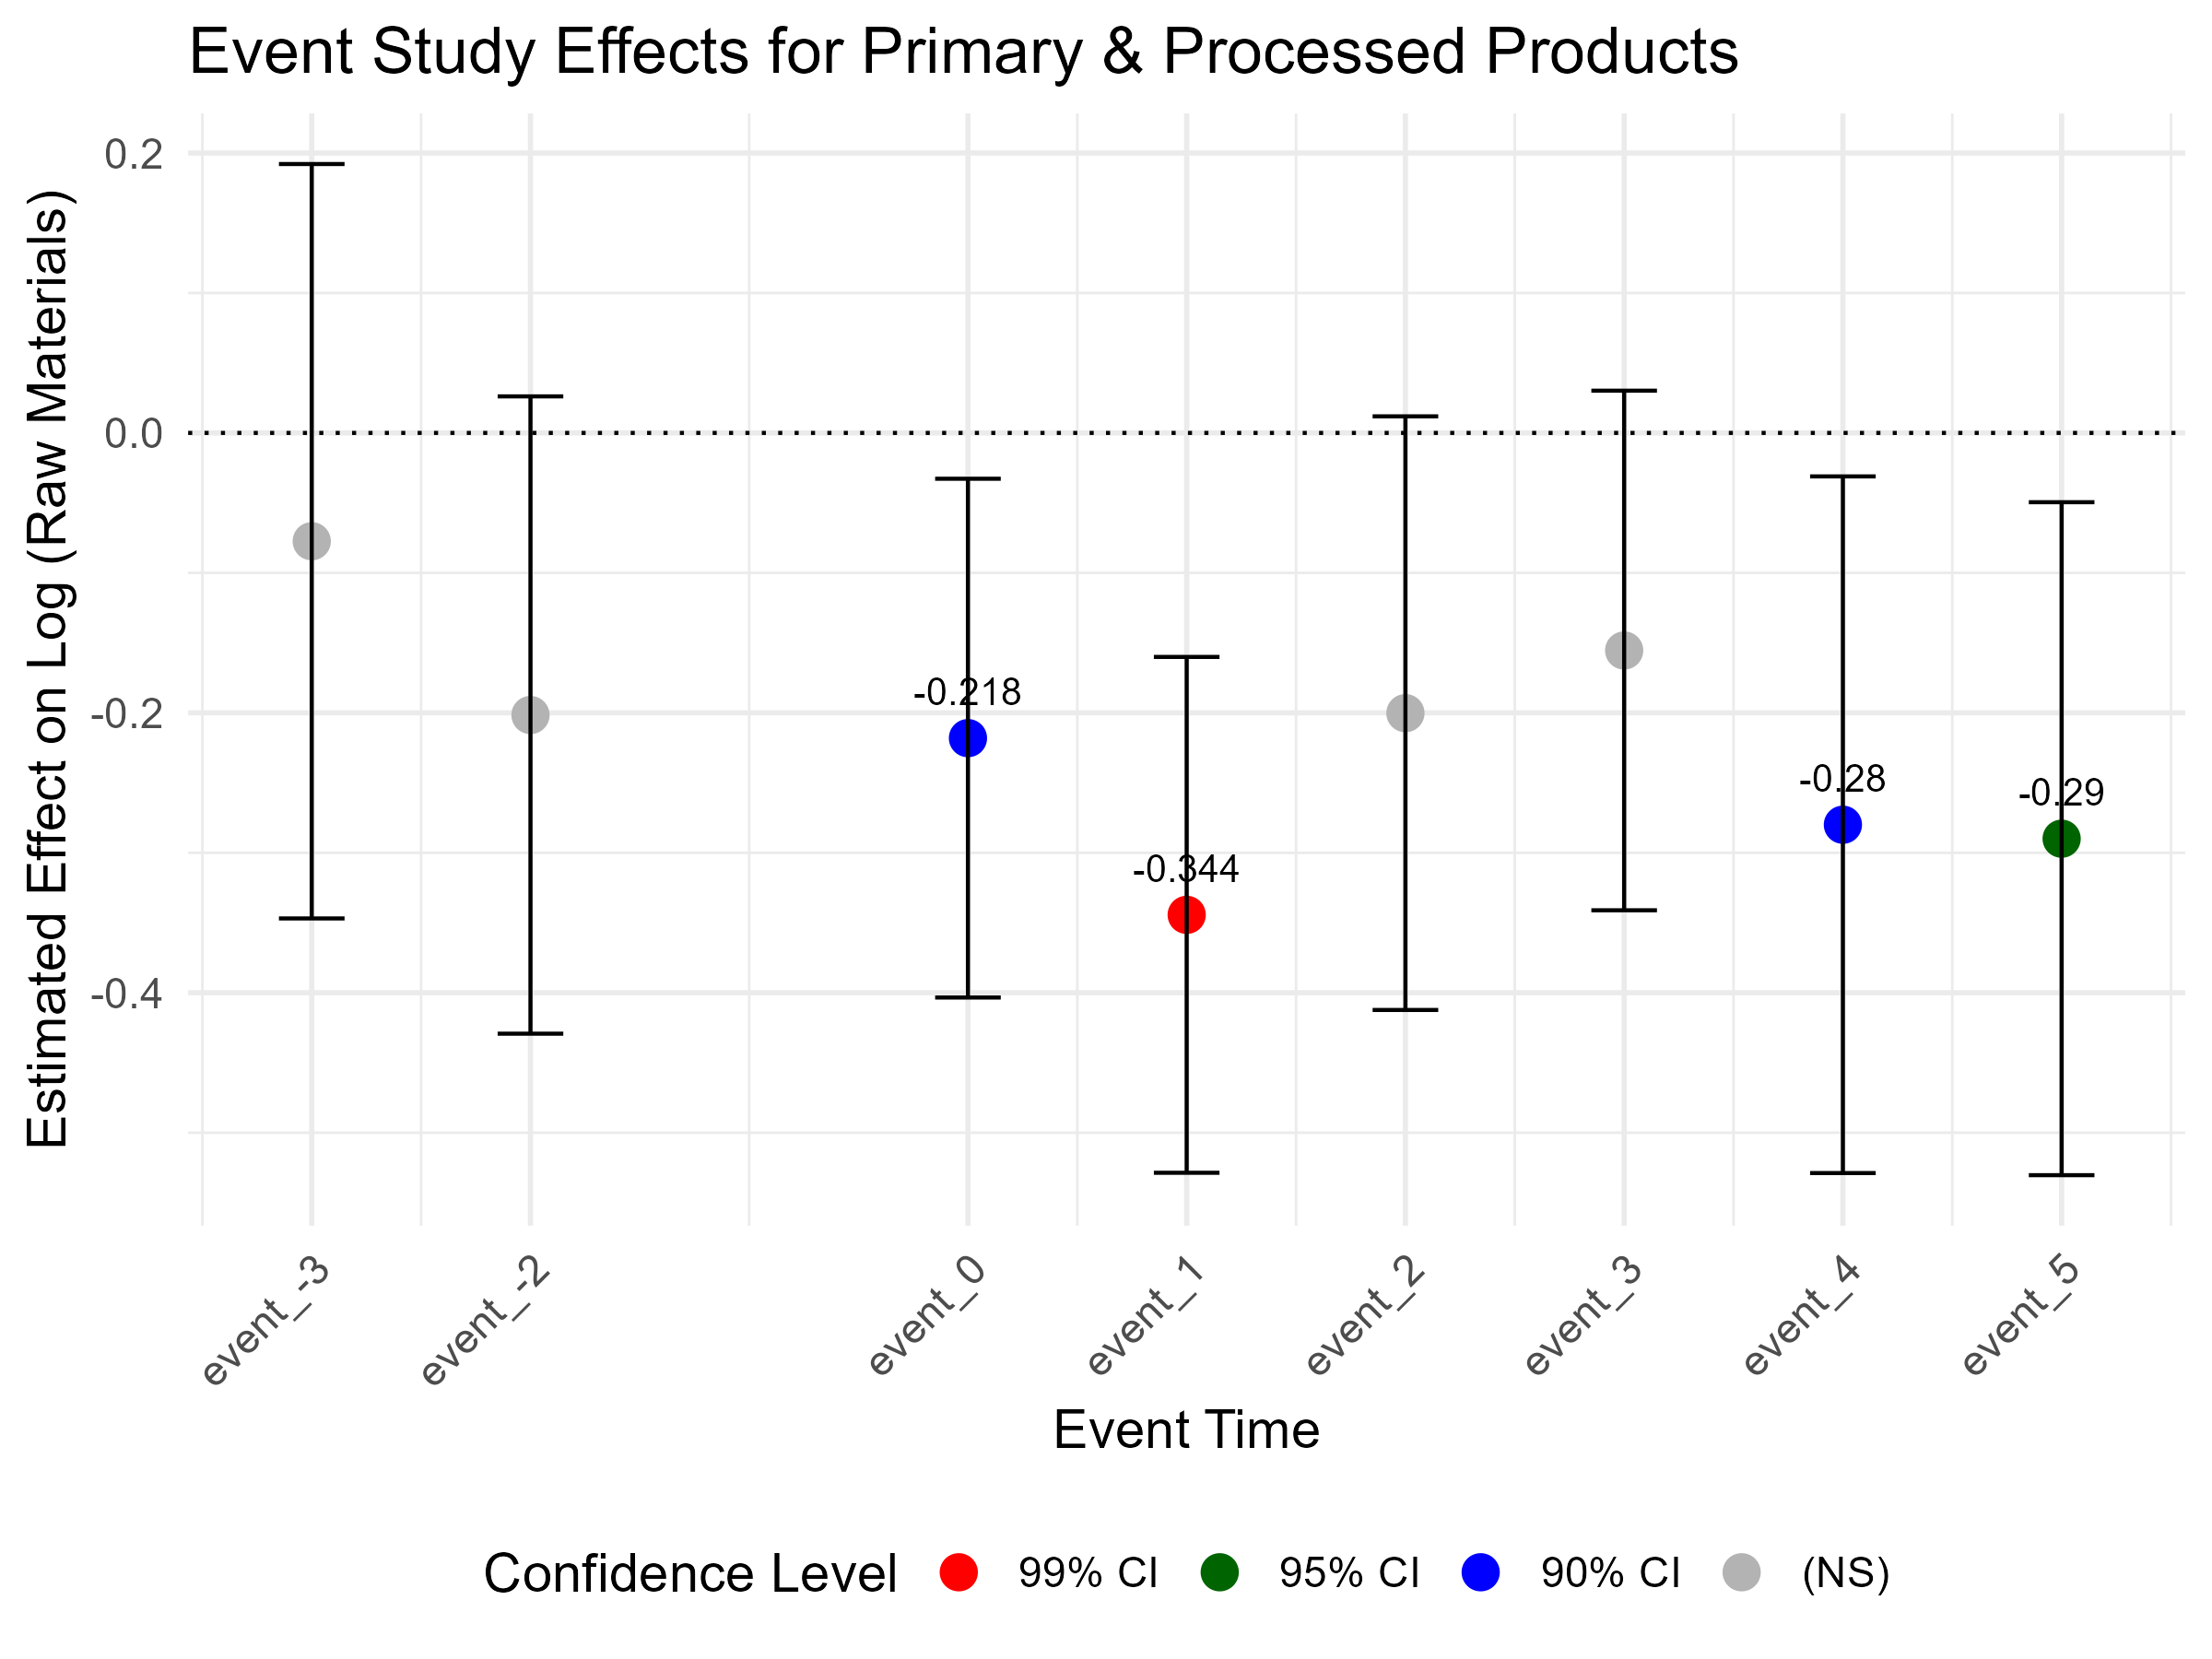
\includegraphics[width=0.55\linewidth]{PrimIndustriesRawM.png}
        \caption{Impact of Extreme Natural Disasters on Raw Materials of Primary \& Processed products firms}
        \label{fig:RawMPrim}
    \end{figure}

\subsection{Placebo Tests}

The purpose of this subsection is to assess the exogeneity of extreme disasters. I follow the theoretical framework developed by \cite{Hagemann2019}. It introduces a Fisher-style randomization framework for inference in cluster-level treatment. This framework fits this study, as extreme disasters (treatments) do occur at the state level (cluster). I ran the mode 500 times under random assignments (years and states), preserving the number of states affected. Basically, I want to ensure that the true estimate is not randomly distributed within the placebo estimates, which would mean that the effect I estimated was random. Figures (\ref{fig:Placebo_prim},\ref{fig:Placebo_lightmanuf},\ref{fig:Placebo_machcap},\ref{fig:Placebo},\ref{fig:Placebo_chem}) represent the distribution of the placebo coefficient (\color{gray}{in gray}\color{black}) and the true estimated coefficient (\color{red}{red-dotted line}\color{black}). I will present the case of primary and processed firms\footnote{the other ones can be found in the appendices in Figure\ref{fig:Placebo_lightmanuf},\ref{fig:Placebo_machcap},\ref{fig:Placebo_chem},\ref{fig:Placebo}}.

\begin{figure}[H]
        \centering
        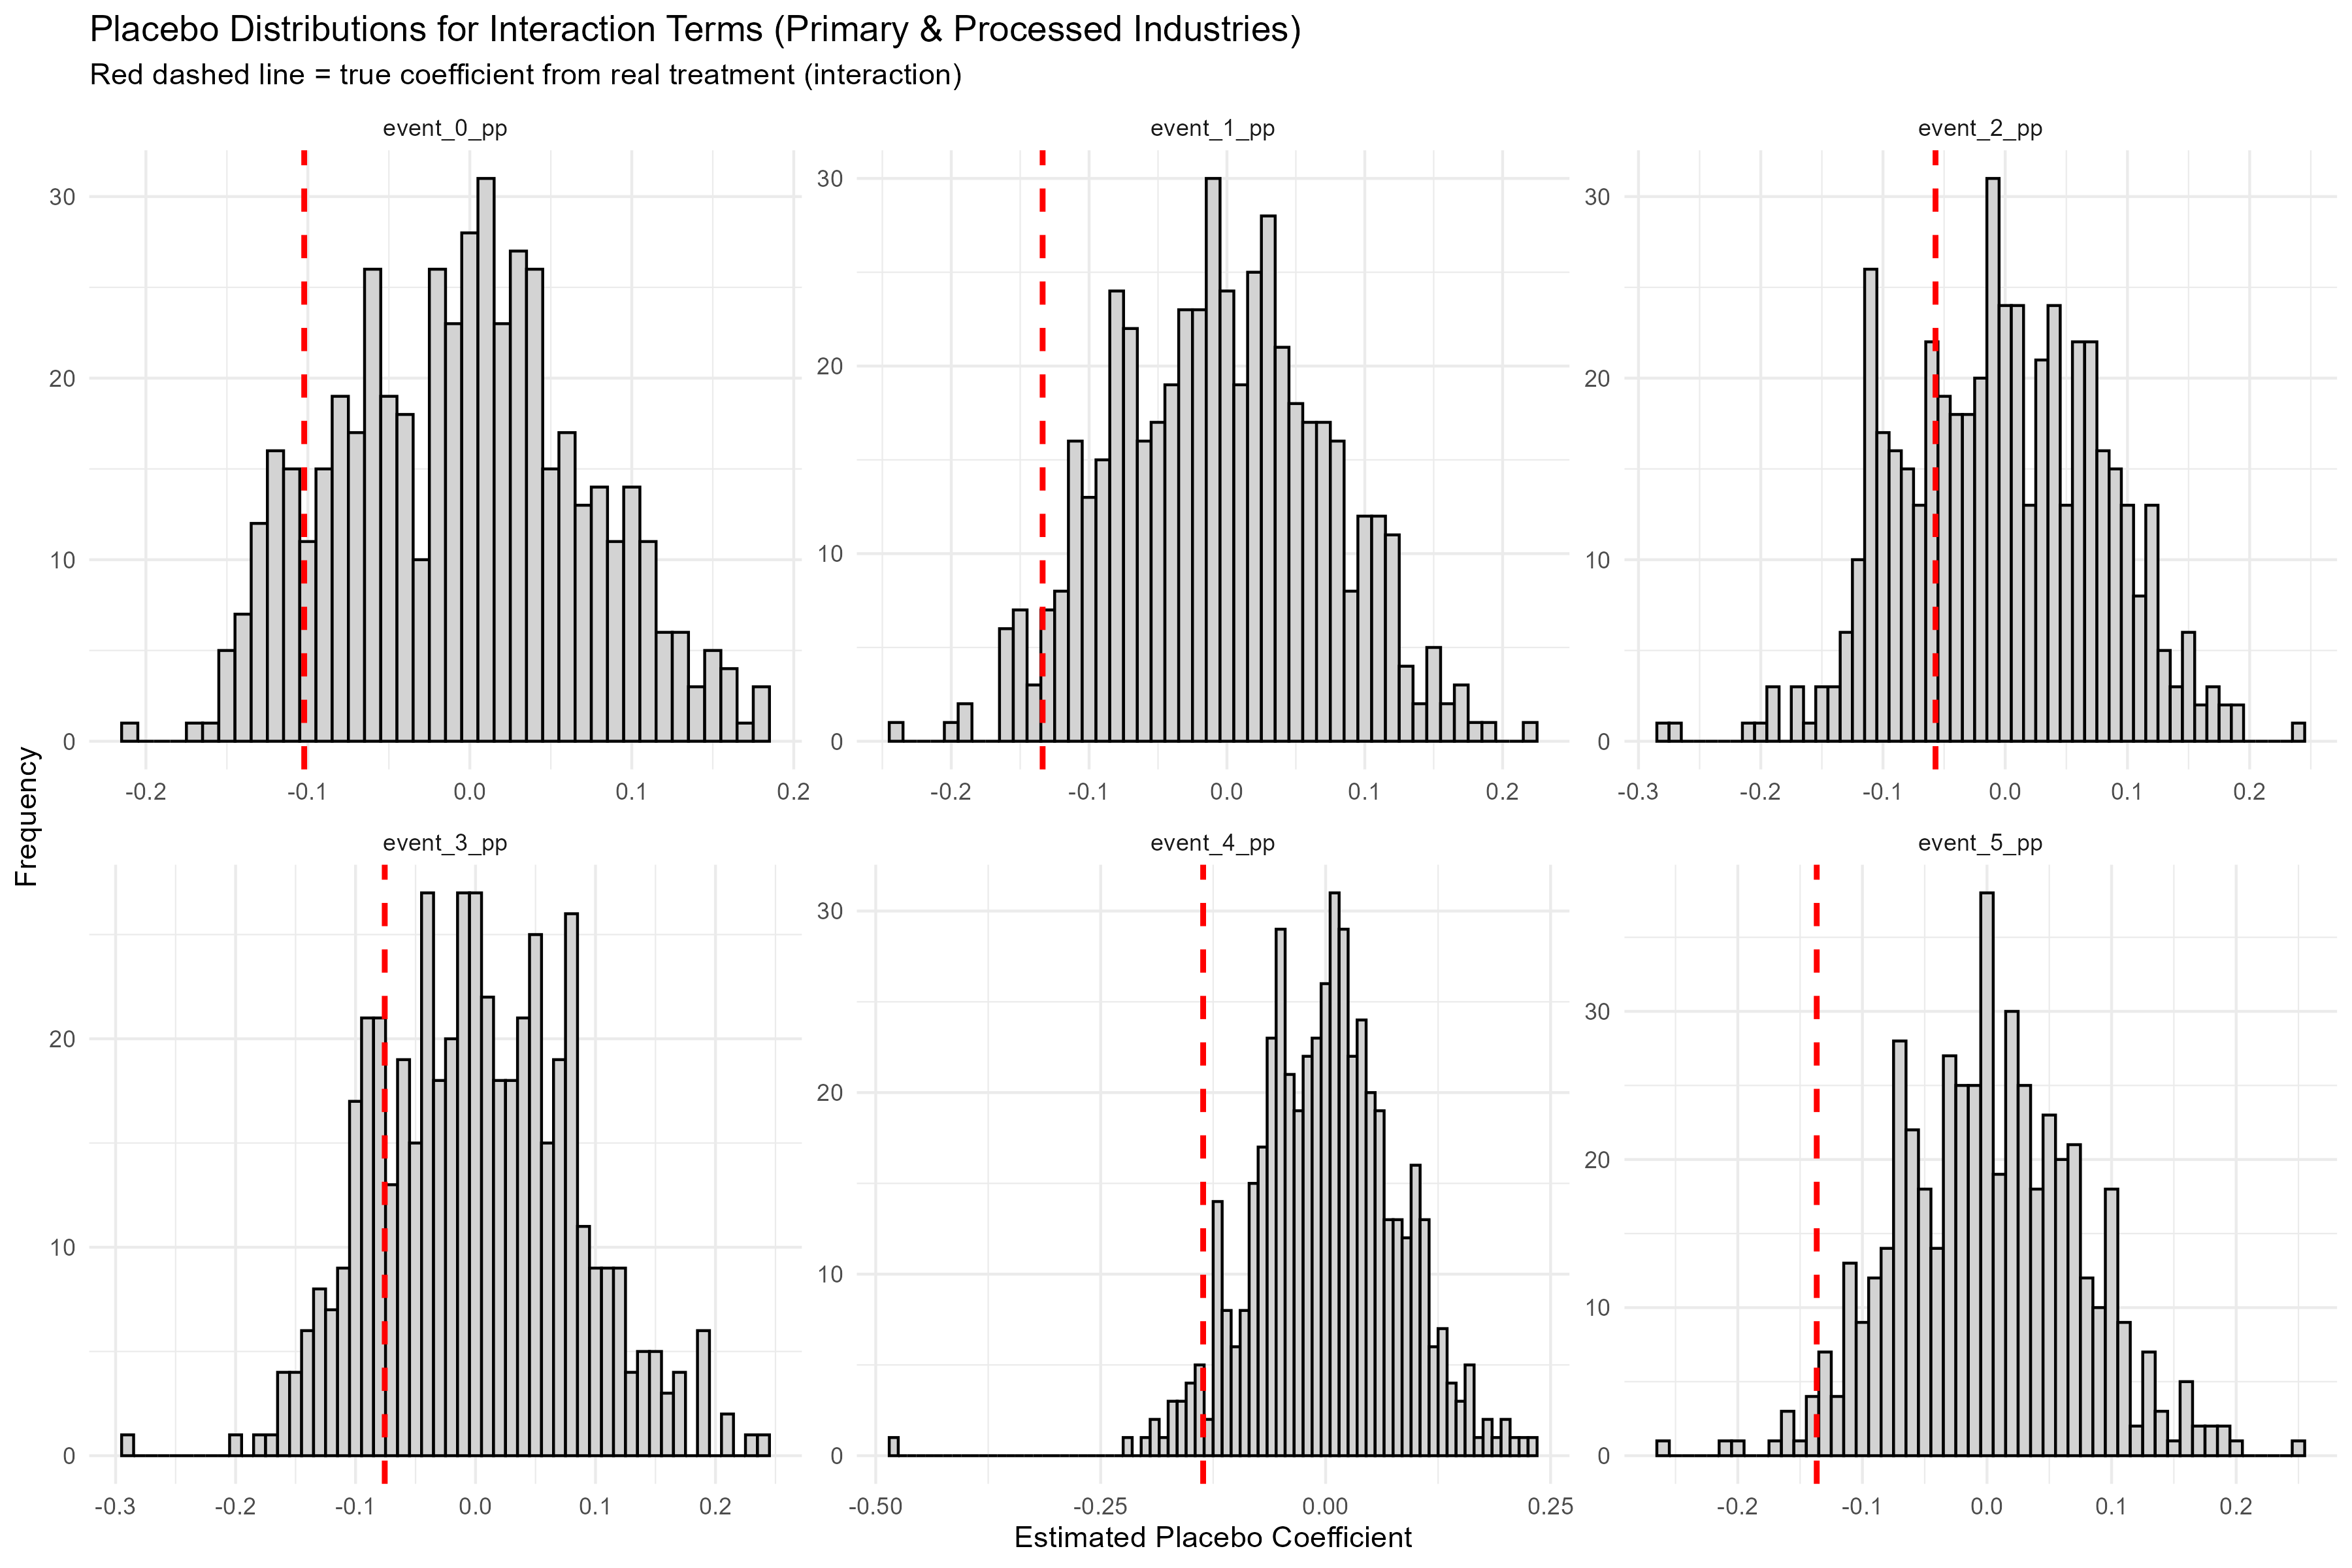
\includegraphics[width=1\linewidth]{placebo_PrimIndus.png}
        \caption{Distribution of coefficient of Placebo tests for each event period (Primary \& Processed Firms)}
        \label{fig:Placebo_prim}
    \end{figure}

As we can see in the figure \ref{fig:Placebo_prim}, the true estimate lies in the tail of the distribution of placebo estimates, which rules in favor of a true effect of natural disasters on primary \& processed firms. This can be further confirmed by the table \ref{tab:placebo_pvalues_prim} showing the p-values of the true estimate. Since all of them are greater than 0.10, I can affirm that they are not randomly distributed.

\begin{table}[H]
\centering
\caption{Empirical p-values from placebo test using random treatment assignment across clusters (Primary \& Processed firms).}
\begin{tabular}{lcc}
\hline
\textbf{Event Time} & \textbf{True Coefficient} & \textbf{p-value} \\
\hline
event\_0 & -0.1023 & 0.880 \\
event\_1 & -0.1337 & 0.958 \\
event\_2 & -0.0570 & 0.720 \\
event\_3 & -0.0757 & 0.802 \\
event\_4 & -0.1361 & 0.962 \\
event\_5 & -0.1367 & 0.976 \\
\hline
\end{tabular}
\label{tab:placebo_pvalues_prim}
\end{table}

\section{Discussions}

In this section, I will discuss the implications of the results of this study. First, I show that it is mainly firms in upstream industries that are negatively affected by natural disasters. This finding holds for different specifications and for controlling for many potential confounders. I do not find any evidence for the Schumpeter' Creative Destruction theory as in the long run results seem to be not significant for these upstream industries. However, I observe this trend for downstream industries (columns 1 and 4 of Table \ref{tab:main_interactions}). Indeed, these positive results in the medium and long term rule for the presence of this economic boom after a disaster. We could expect it since these industries are drivers of the reconstruction of destroyed areas. \\

Concerning the international sourcing of inputs as a channel of adaptation, I cannot argue for the presence of this destructive creation theory, as the performance of these firms does not seem to have been negatively affected. This leads us to an important point to address, the yearly basis of the study. Some previous work has shown that some companies negatively affected by disasters were able to recover within the year after the disaster \citep{Berkel2021}. Our data being at the year level, I am unable to observe the dynamics within the year of the event. Therefore, I might miss an even shorter-time effect for these downstream industries.
Another caveat of this study is the financial constraints facing firms. Indeed, I am able to control for the financial constraints at the industry level with our sector-year fixed effects, but our proxy at the firm level (leverage ratio) can omit a certain aspect of these financial constraints. This omission is the ease for firms to have access to financial support (for example, through the presence of banks nearby) and the impact it can have on its recovery patterns. \\

In terms of generalization of the results, we have to be careful in their interpretation. Studies in other contexts have found results that can differ in magnitude, but also in sign of the effect of natural disasters. An important finding of this literature is that more developed countries were able to foster economic recovery more effectively mainly due to the quality of their institutions and the high development of their financial networks. Therefore, these results can be used for regions prone to disasters that are closer to the Indian regions affected.

\newpage
\section{Conclusion}

This paper aims to contribute to the literature by assessing the impact of extreme natural disasters on firms' performance in India. Using the six greatest disasters that occurred during the 1990s, I show that firms in upstream industries are the most affected by natural disasters. This effect lasts up to four years after the disaster. In addition, sourcing input from abroad appears to be an effective way for a company to create resilient adaptation mechanisms. These results are robust across different specifications with alternative outcomes of firm performance and throughout placebo estimates. \\

Beyond its implication for the academic literature, these findings may also be useful for policy implications. In the context of the rising concerns drawn by natural disasters, understanding which firms and industries are the most at risk, along with which levers a public planner can use as adaptation mechanisms, matters. \\

This study is intended to be a signal for future research. Indeed, the data used are now more than 20 years old. Since 1990, global temperatures have increased by almost a degree compared to preindustrial times (1850s). This means that today we are in a world much more prone to natural disasters of greater intensity. Future research is required to update these findings and help both companies and governments adapt to their decisions to new living conditions. 


\newpage
\bibliography{references}

\section{Appendices}

\subsection*{Summary Statistics per Industry}

\begin{table}[H]
\centering
\caption{Summary Statistics by Industry}
\resizebox{\textwidth}{!}{%
\begin{tabular}{rlrrrrrrrrrrrr}
  \toprule
  & \textbf{Sector} & \textbf{Log Sales} & \textbf{Imports} & \textbf{Interm.} & \textbf{Raw} & \textbf{Capital} & \textbf{Exports} \\
  \midrule
1 & Books & 4.13 & 21.86 & 0.29 & 20.21 & 1.34 & 3.12 \\ 
  &       & (1.57) & (38.15) & (0.62) & (36.14) & (5.41) & (8.33) \\
2 & Food Products & 4.35 & 9.44 & 0.24 & 6.95 & 0.48 & 9.46 \\
  &       & (1.49) & (62.16) & (1.16) & (56.85) & (2.87) & (40.94) \\
3 & Textiles & 3.86 & 9.03 & 0.94 & 5.16 & 2.80 & 25.61 \\
  &       & (1.35) & (27.79) & (2.90) & (18.36) & (9.81) & (51.62) \\
4 & Wood \& Wood Products & 1.76 & 0.00 & 0.00 & 0.00 & 0.00 & 0.00 \\
  &       & (0.66) & (0.00) & (0.00) & (0.00) & (0.00) & (0.00) \\
5 & Paper \& Paper Products & 3.58 & 2.82 & 0.24 & 2.26 & 0.32 & 0.80 \\
  &       & (1.12) & (5.60) & (0.89) & (5.22) & (1.02) & (2.99) \\
6 & Leather \& Leather Products & 3.42 & 7.05 & 0.68 & 4.38 & 1.71 & 27.95 \\
  &       & (1.29) & (14.06) & (1.92) & (8.84) & (9.43) & (39.96) \\
7 & Rubber \& Plastic Products & 3.14 & 8.07 & 0.61 & 5.11 & 2.53 & 8.62 \\
  &       & (1.51) & (25.79) & (3.78) & (15.63) & (14.14) & (30.14) \\
8 & Chemicals \& Chemical Products & 3.82 & 20.81 & 0.53 & 17.79 & 1.93 & 32.71 \\
  &       & (1.94) & (60.76) & (2.37) & (53.74) & (10.48) & (167.66) \\
9 & Non-Metallic Mineral Products & 4.35 & 26.10 & 4.34 & 14.94 & 5.19 & 15.18 \\
  &       & (1.94) & (87.01) & (18.69) & (59.48) & (16.35) & (48.92) \\
10 & Basic Metals \& Metal Products & 4.01 & 41.75 & 3.75 & 33.31 & 4.84 & 25.11 \\
  &       & (1.74) & (238.26) & (24.00) & (205.43) & (40.46) & (124.57) \\
11 & Machinery \& Machine Tools & 3.54 & 25.72 & 7.93 & 14.52 & 1.63 & 8.49 \\
  &       & (1.76) & (129.63) & (70.68) & (61.64) & (7.77) & (43.77) \\
12 & Transport Equip. \& Parts & 4.33 & 41.38 & 5.88 & 30.32 & 5.44 & 18.20 \\
  &       & (1.69) & (178.76) & (27.95) & (140.55) & (34.81) & (70.49) \\
13 & Misc. Manufactured Articles & 3.29 & 10.76 & 0.17 & 9.90 & 0.22 & 20.95 \\
  &       & (1.49) & (18.99) & (0.28) & (18.77) & (0.42) & (38.27) \\
\bottomrule
\end{tabular}
} % end resizebox
\label{tab:summary_by_sector}
\end{table}

This table presents the summary statistics. The main difference from the one in the main text lies in the fact that we took all industries in our data set. We can notice that those with the highest sales values are the industries of Books, Food Products, Non-Metallic Mineral Products, Basic Metal \& Metal Products, and Transport Equipments \& Parts industries. 

\subsection*{Maps}

The three maps below present the number of disasters per region between 1990 and 2000, by type of disaster (in \color{RoyalBlue}{blue} \color{black} in \ref{fig:floodsmap}, in \color{orange}{orange} \color{black} in \ref{fig:droughtsmap} \color{ForestGreen}{green} \color{black} in \ref{fig:cyclonesmap}). The objective of these maps is to show that Indian regions are unequally affected by natural disasters. Therefore, using firm location, we can easily create two groups of treated and control, for our Event Study with PSM. Concerning the potential negative correlation between being in a highly affected region and sales growth, the relationship is the clearest on the map showing the distribution of droughts (\ref{fig:droughtsmap}).

\begin{figure}[H]
    \centering
    \begin{subfigure}[b]{0.50\textwidth}
        \centering
        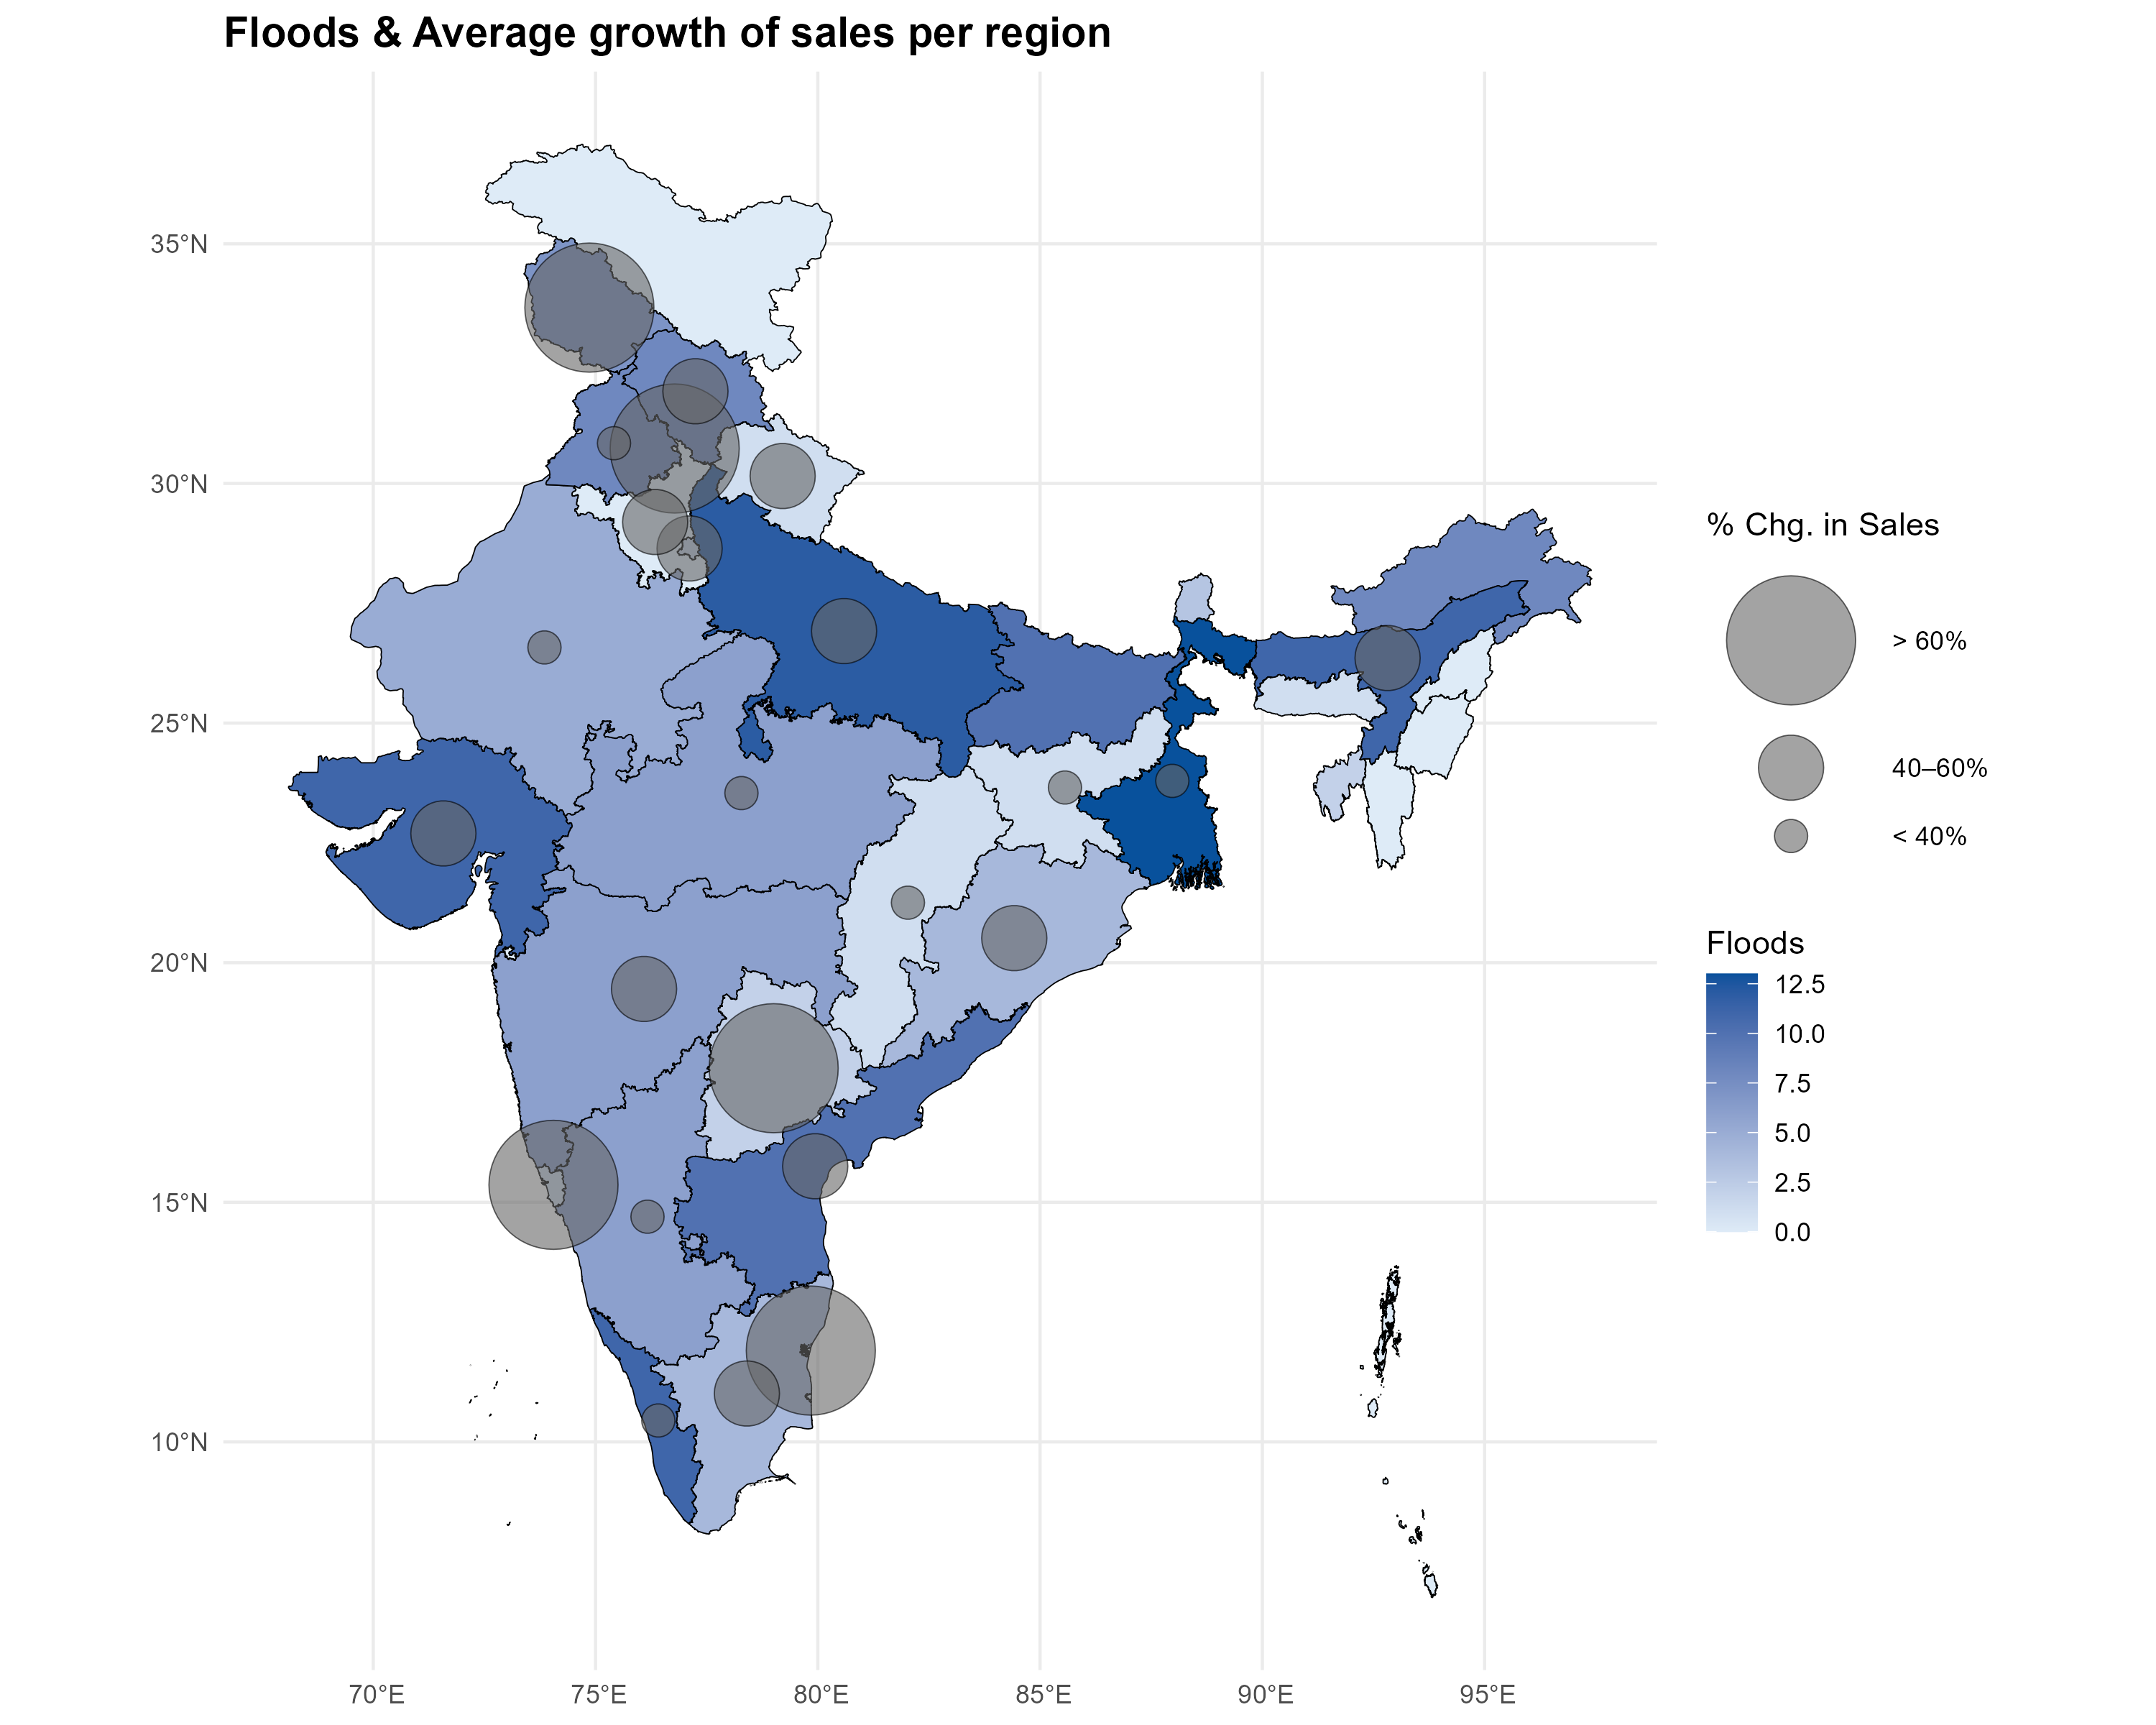
\includegraphics[width=\linewidth]{floods avgsales.png}
        \caption{Floods}
        \label{fig:floodsmap}
    \end{subfigure}
    
    \vspace{0.5cm}
    
    \begin{subfigure}[b]{0.50\textwidth}
        \centering
        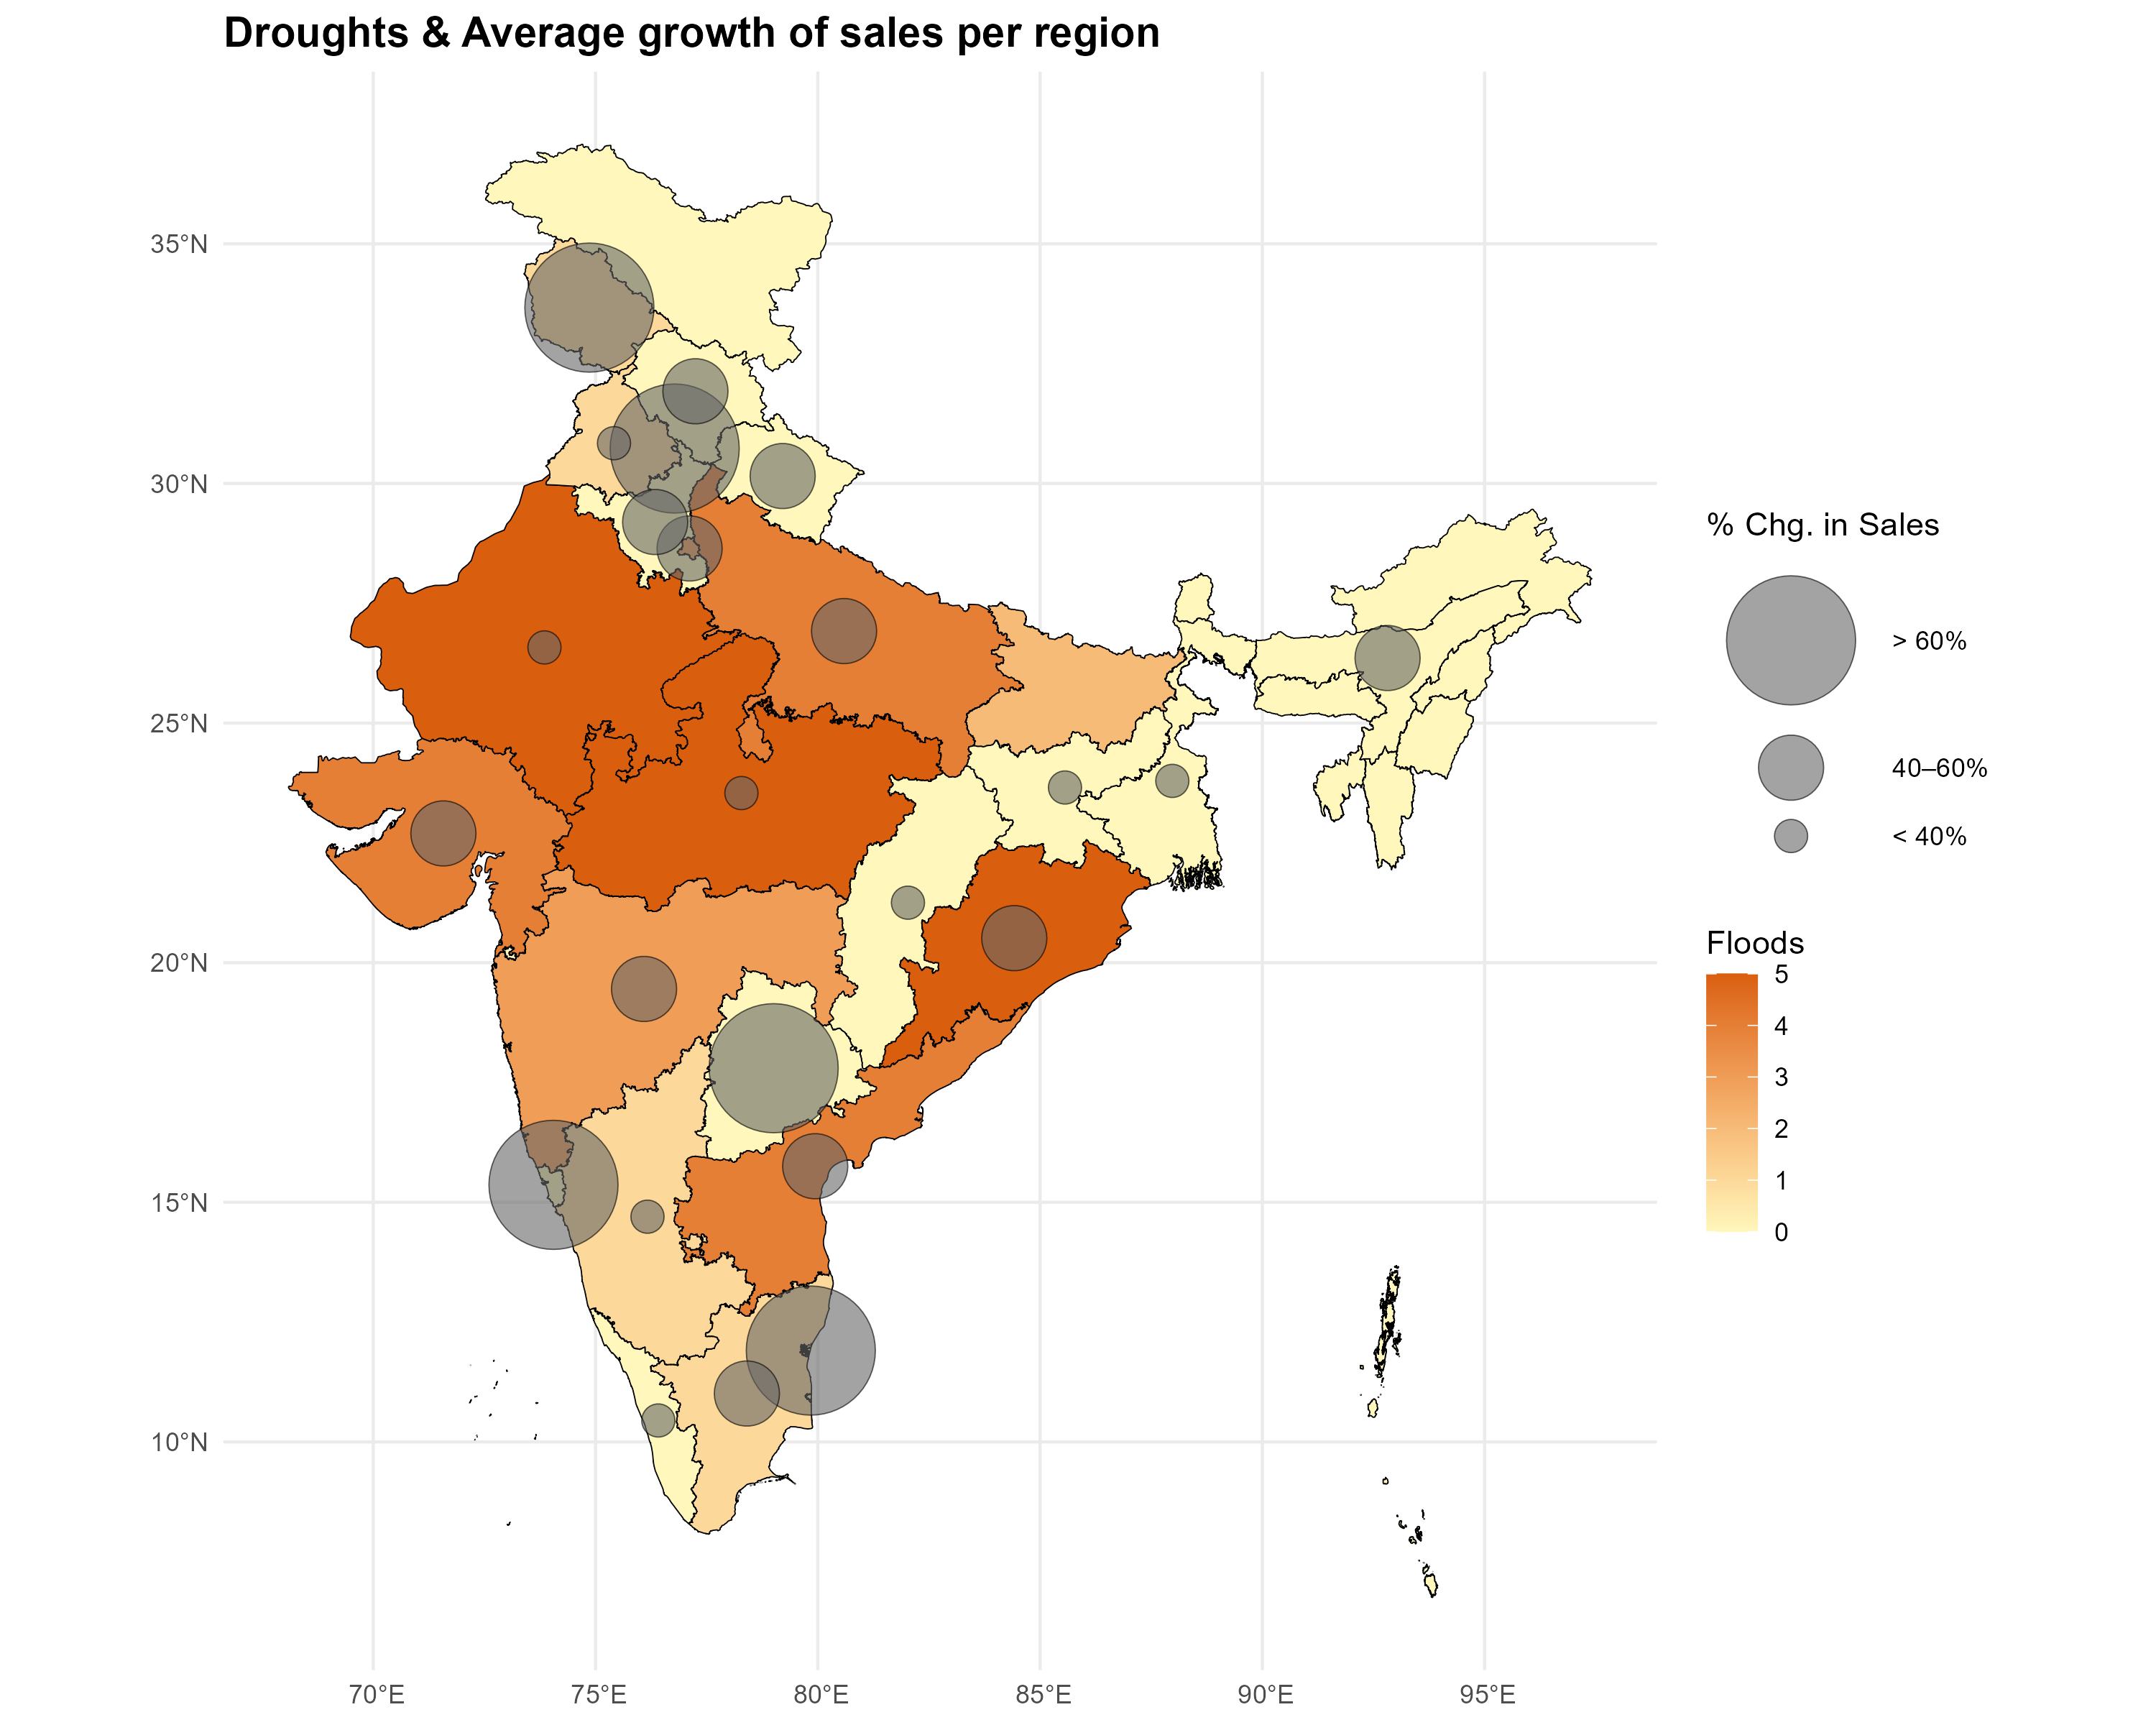
\includegraphics[width=\linewidth]{droughts avgsales.png}
        \caption{Droughts}
        \label{fig:droughtsmap}
    \end{subfigure}
    \hfill
    \begin{subfigure}[b]{.50\textwidth}
        \centering
        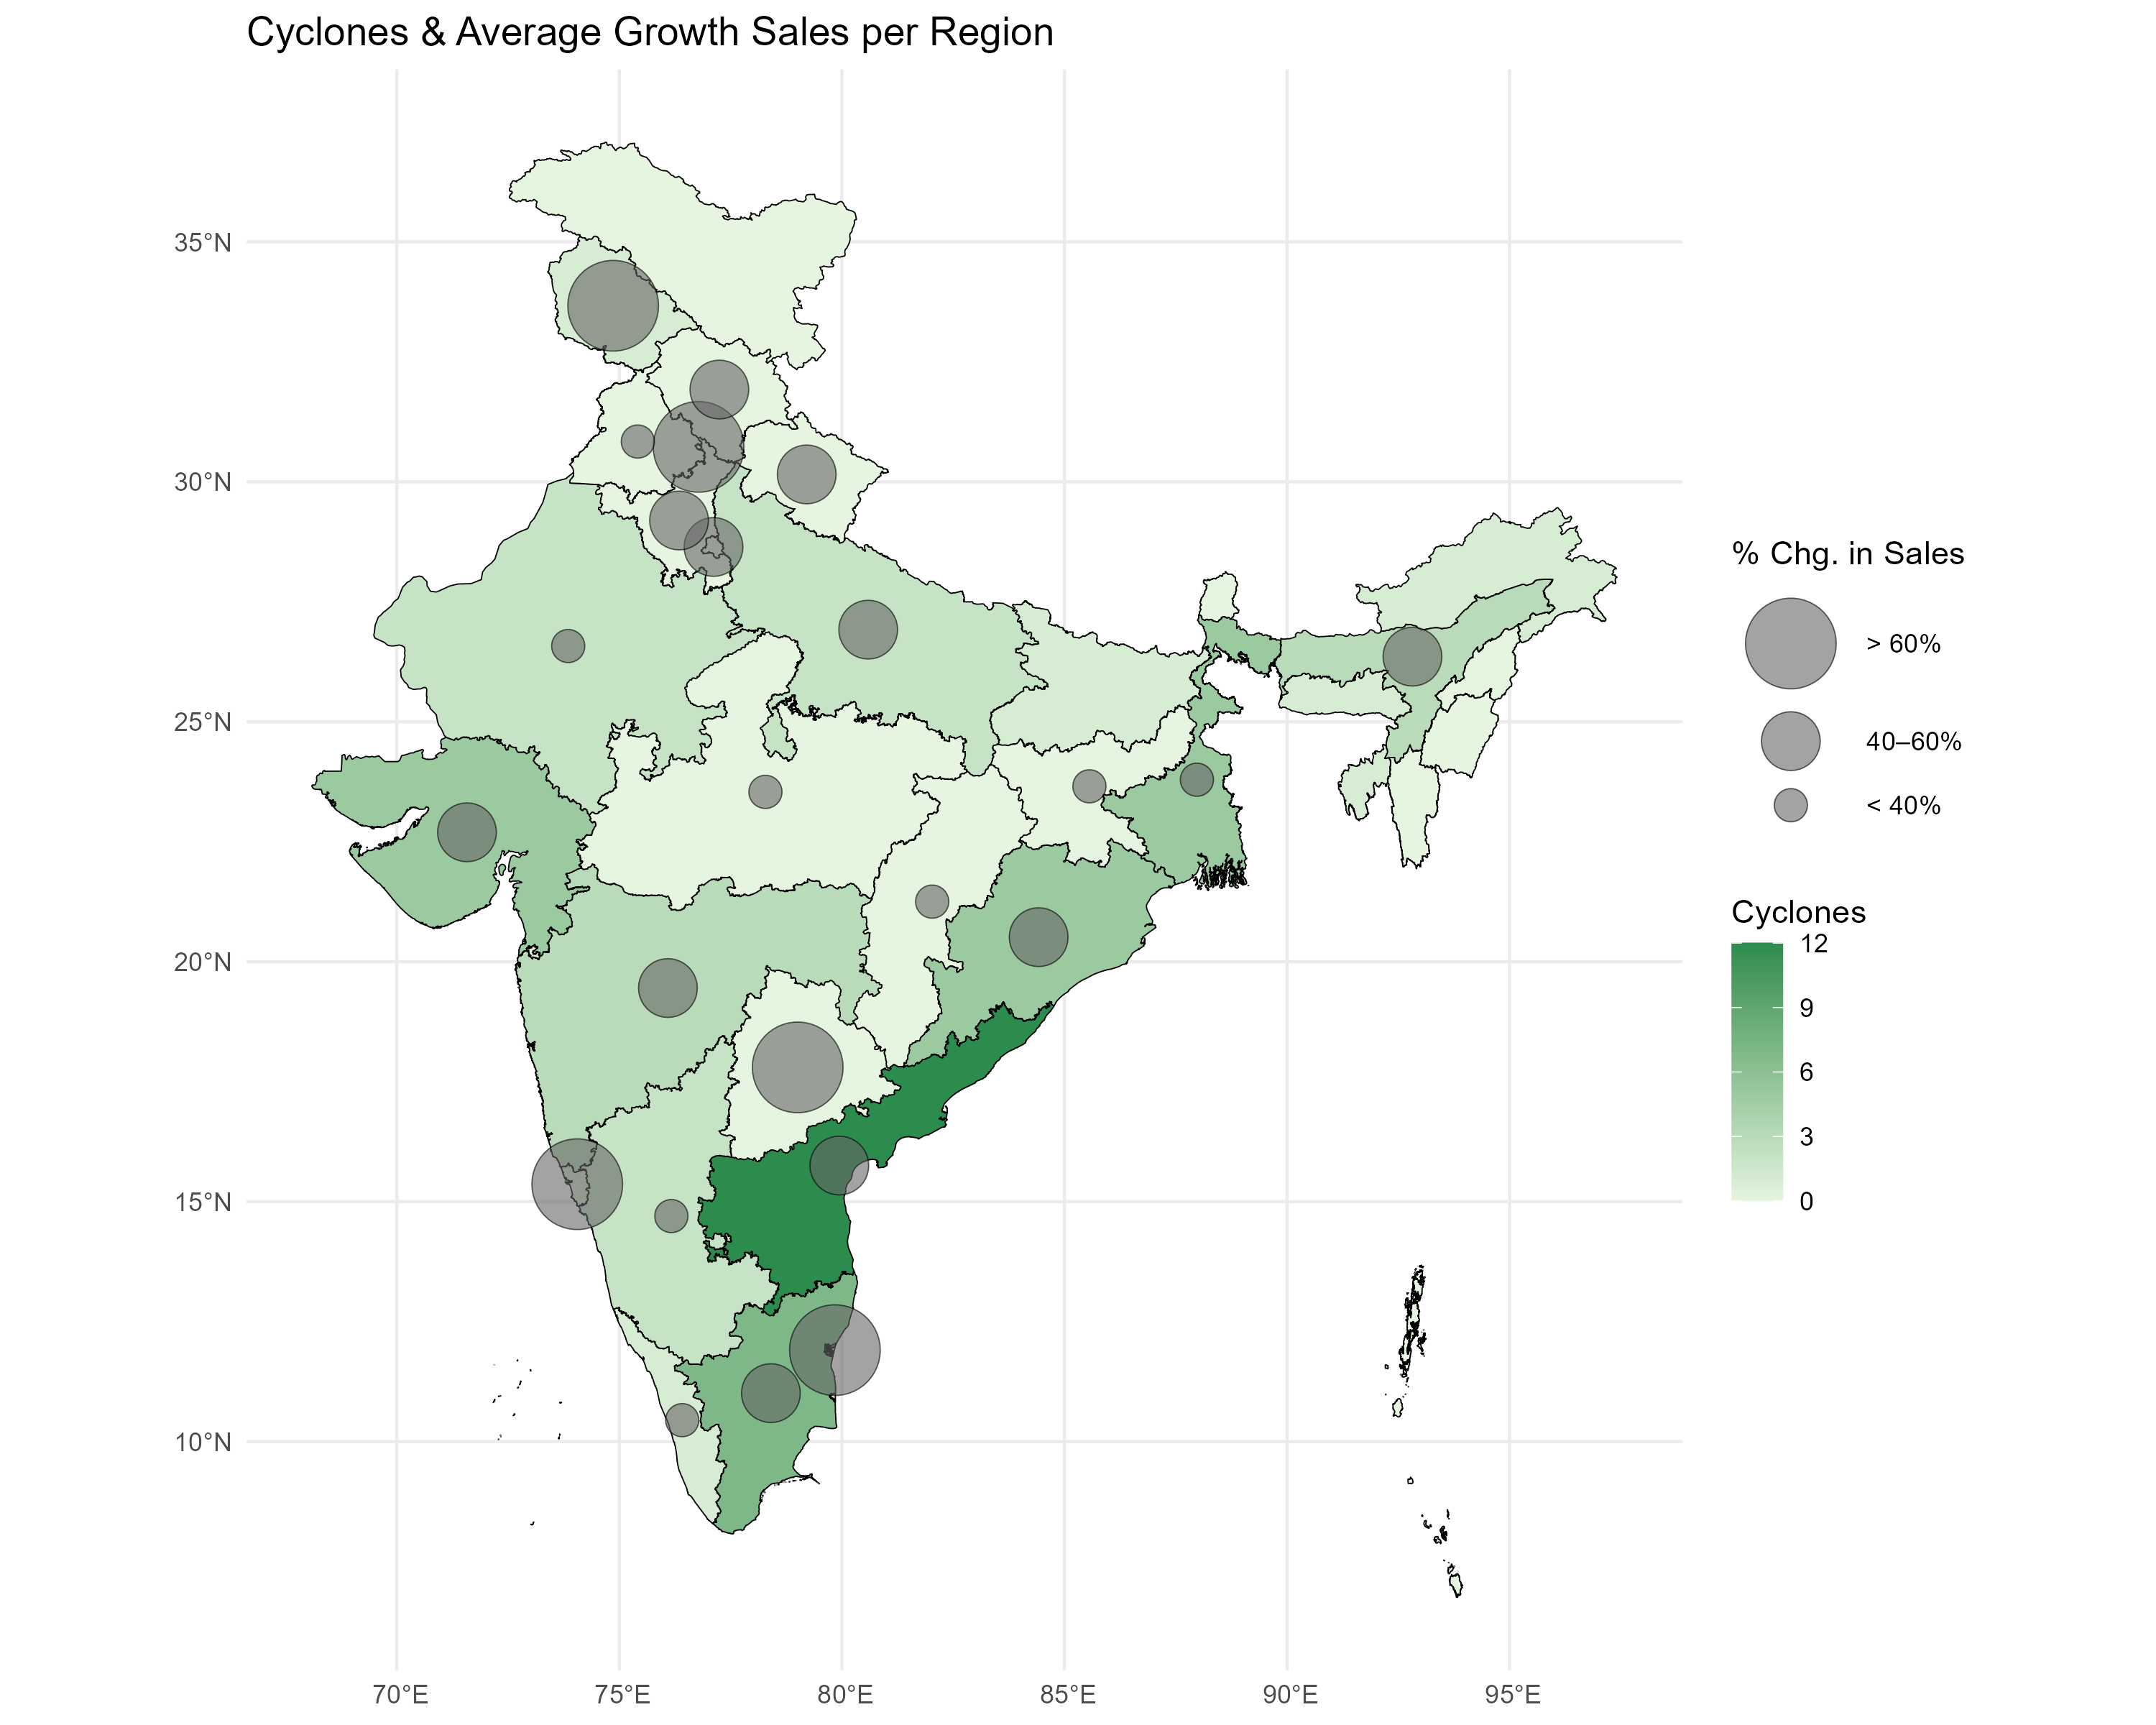
\includegraphics[width=\linewidth]{cyclones avgsales.png}
        \caption{Cyclones}
        \label{fig:cyclonesmap}
    \end{subfigure}
    
    \caption{Natural disasters and firms' sales growth by region}
    \label{fig:disasterspanel}
\end{figure}

\subsection*{Aggregate Event study Results}

\begin{figure}[H]
        \centering
        \caption{Event Study baseline specification}
        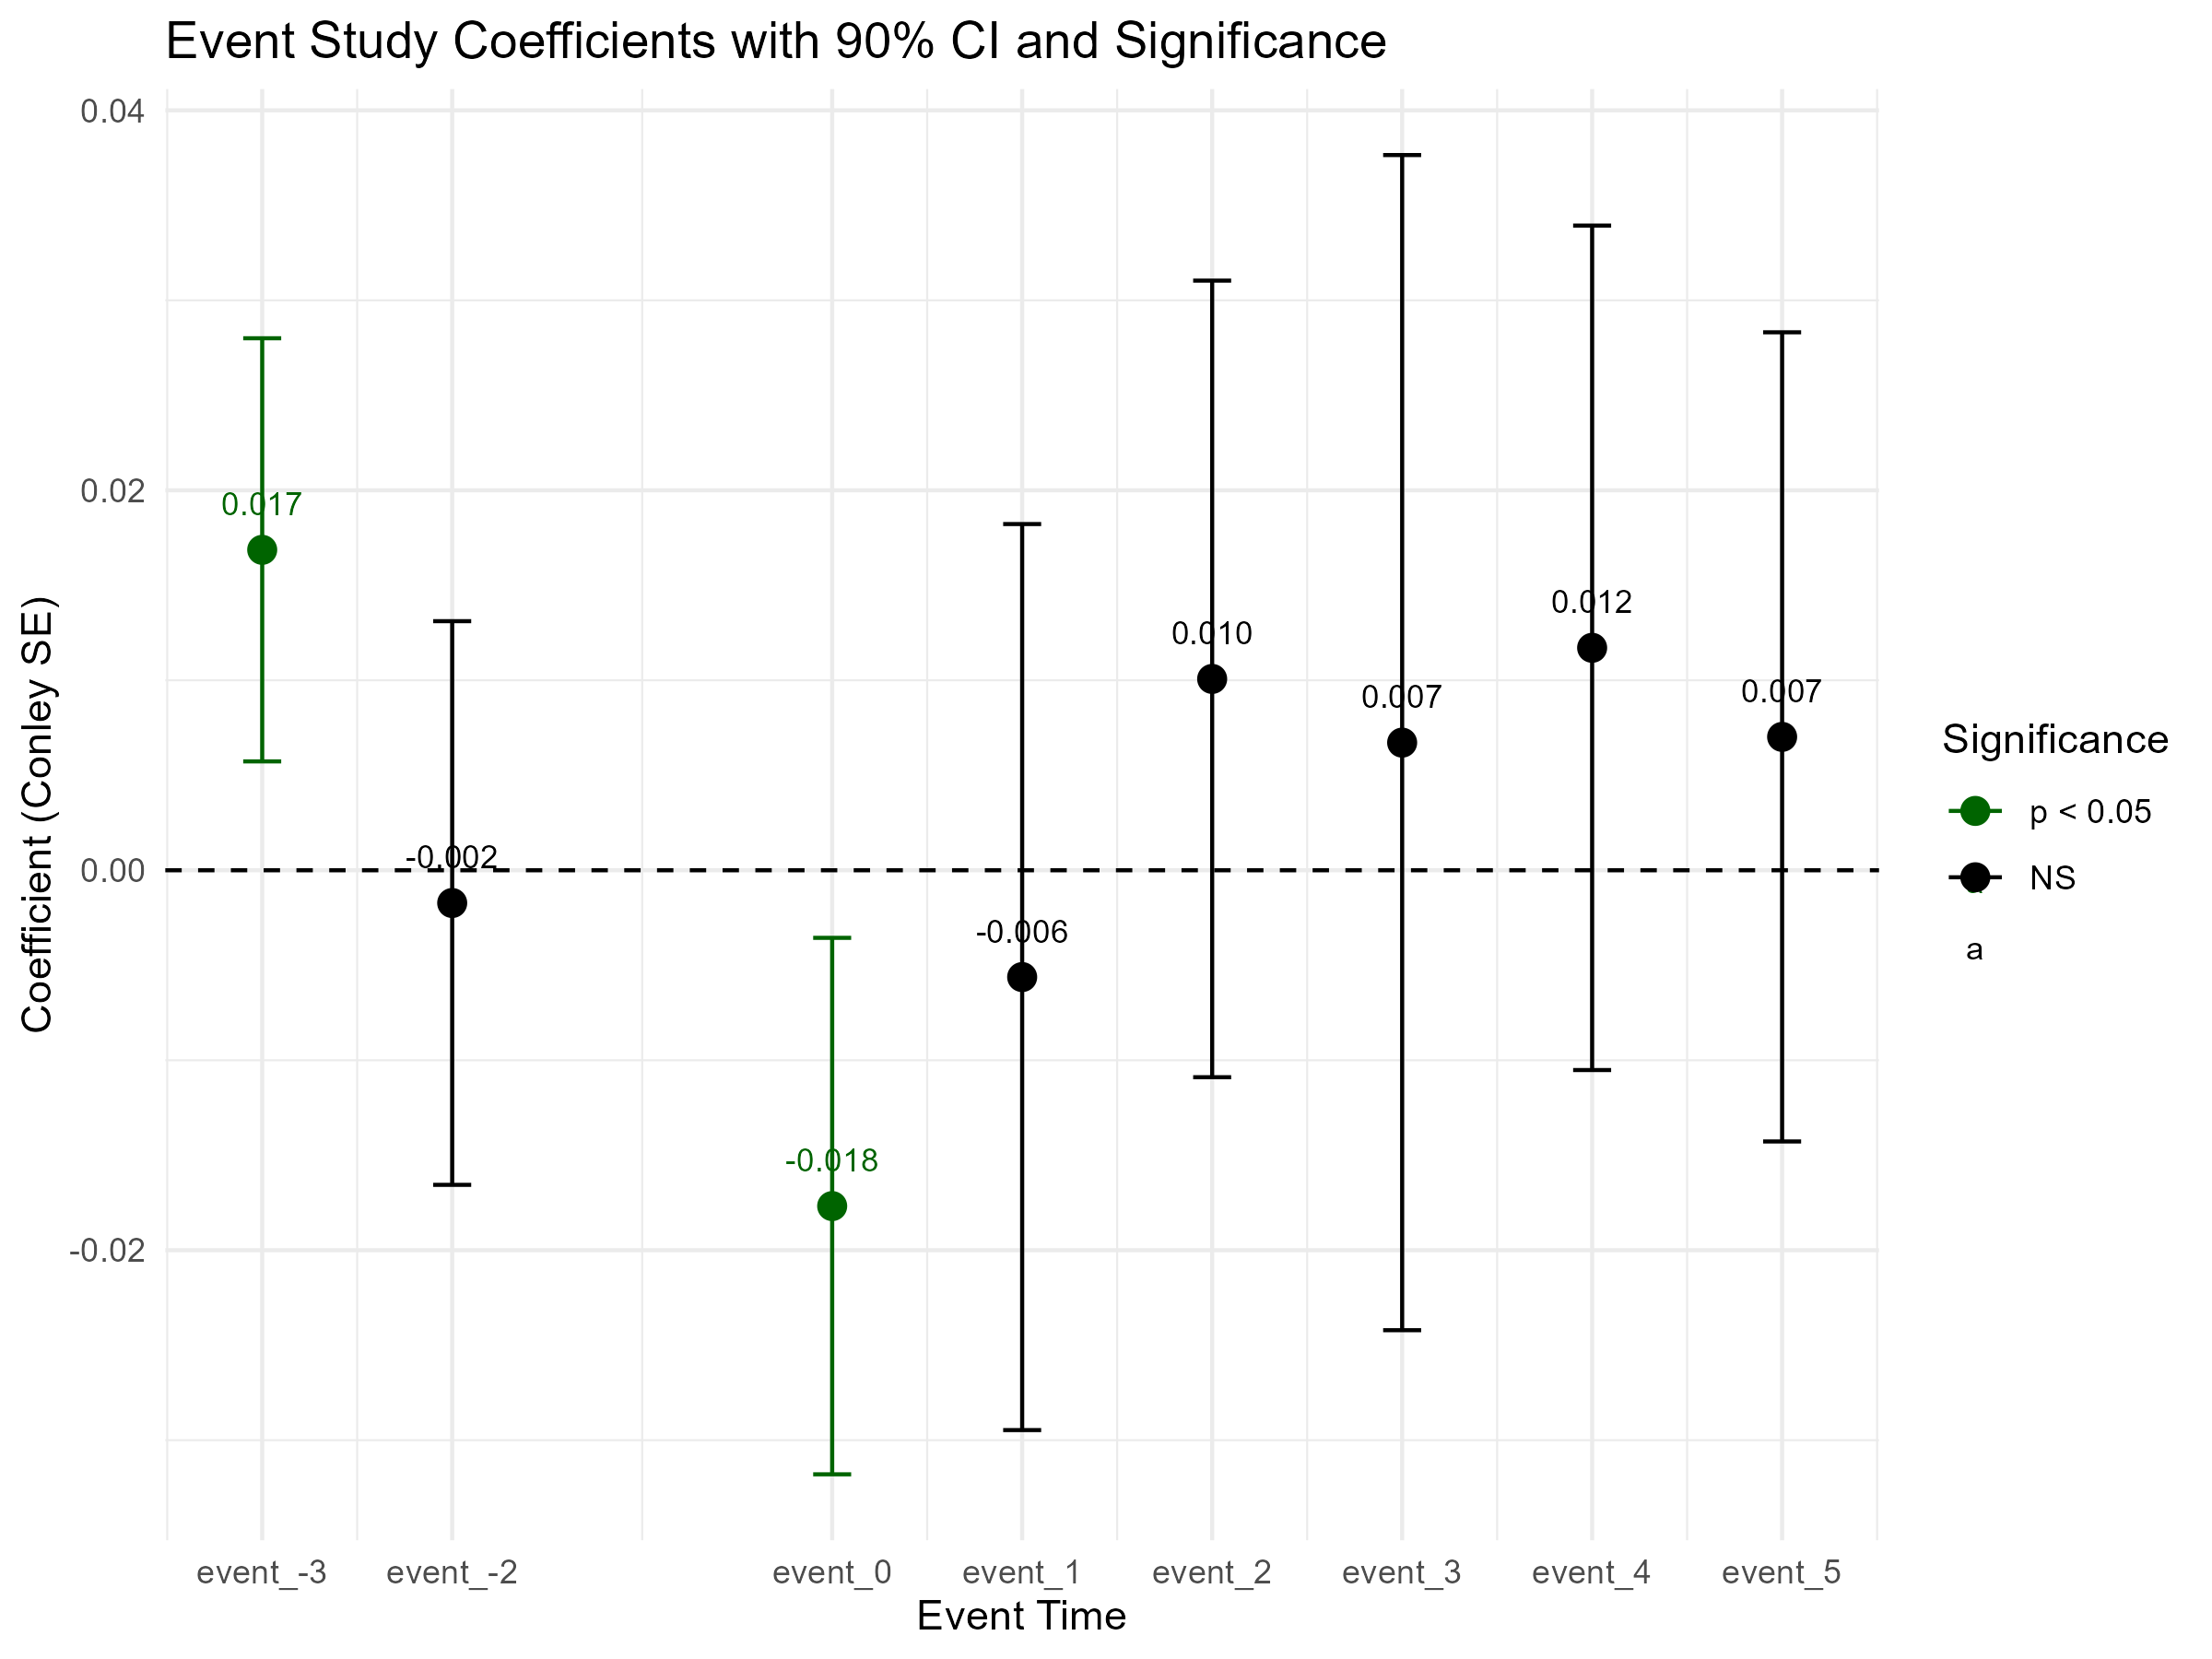
\includegraphics[width=0.55\linewidth]{Pre-trends.png}
        \label{fig:Pre-Trend graph} \\
        Notes: This graph represents the Results of the Event study regression. The outcome variable is the logarithm of sales. The Standard Errors are clustered following the Conley framework at a 100 km grid.
    \end{figure}

\begin{figure}[H]
        \centering
        \caption{Event Study with matching score}
        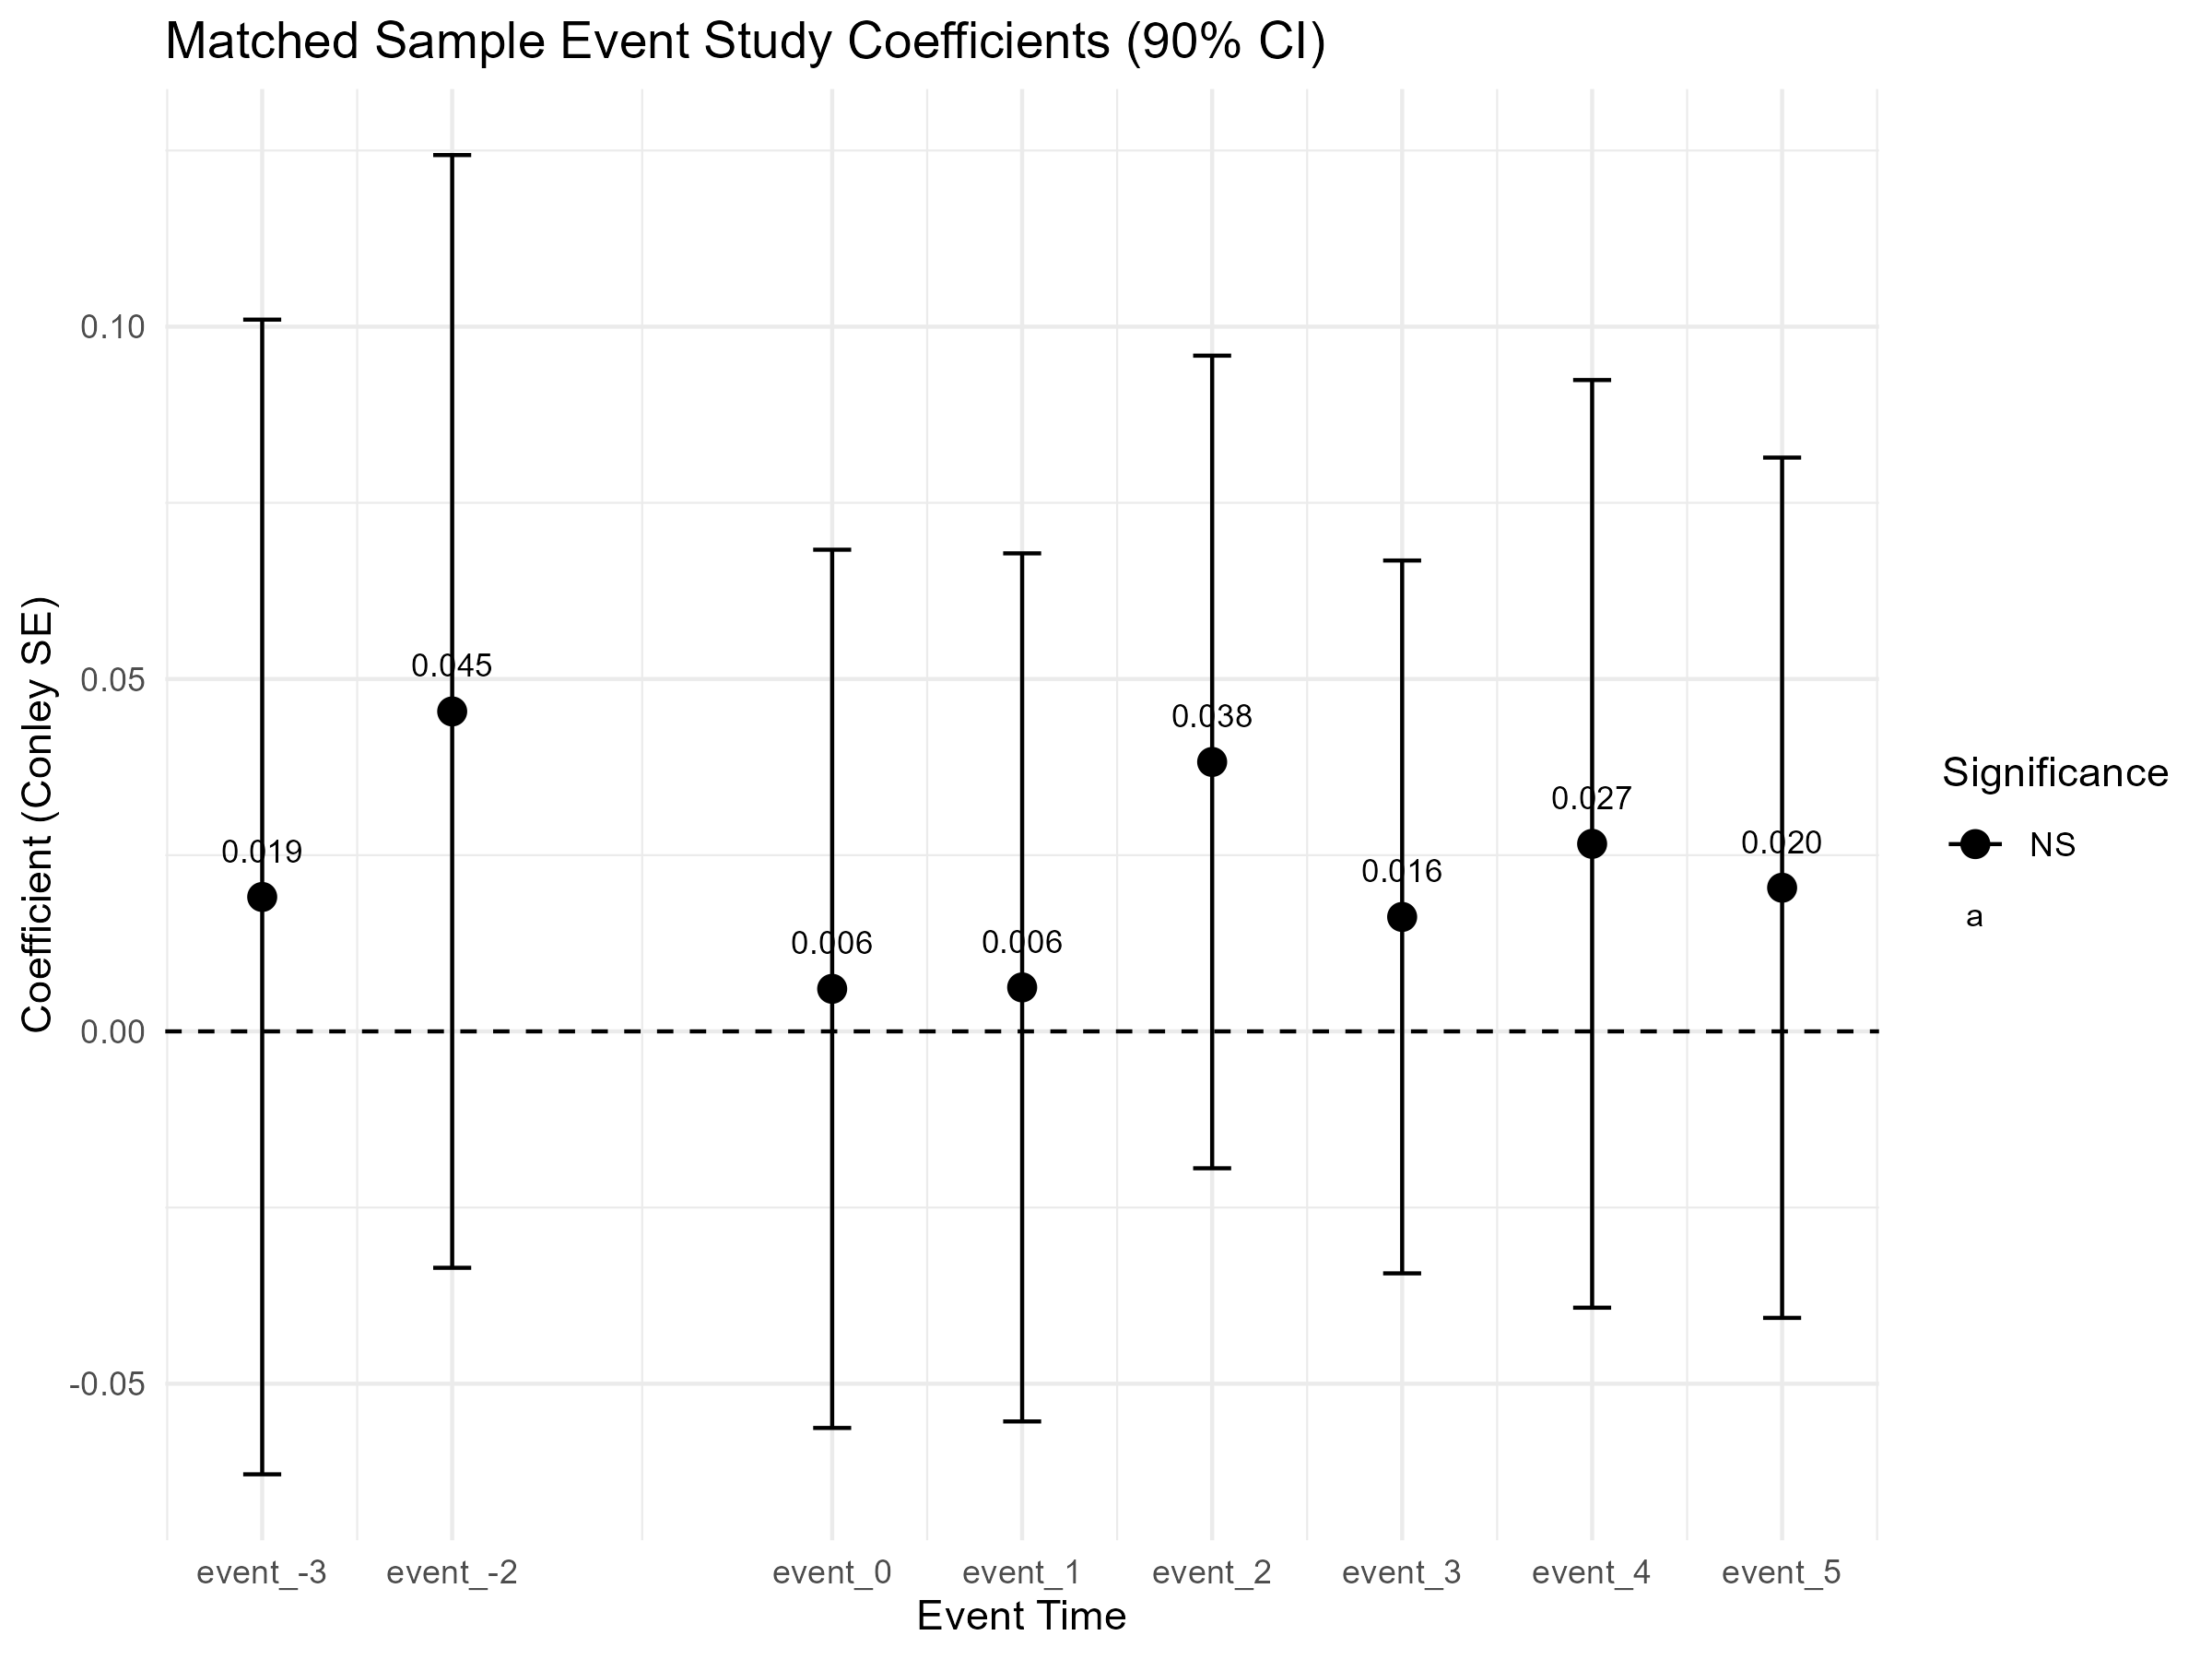
\includegraphics[width=0.55\linewidth]{PSM-Pretrend.png}
        \label{fig:PSM-PreTrend} \\
        Notes: This graph represents the Results of the Event study regression with PSM. The outcome variable is the logarithm of sales. The Standard Errors are clustered following the Conley framework at a 100 km grid.
    \end{figure}

\begin{figure}[H]
        \centering
        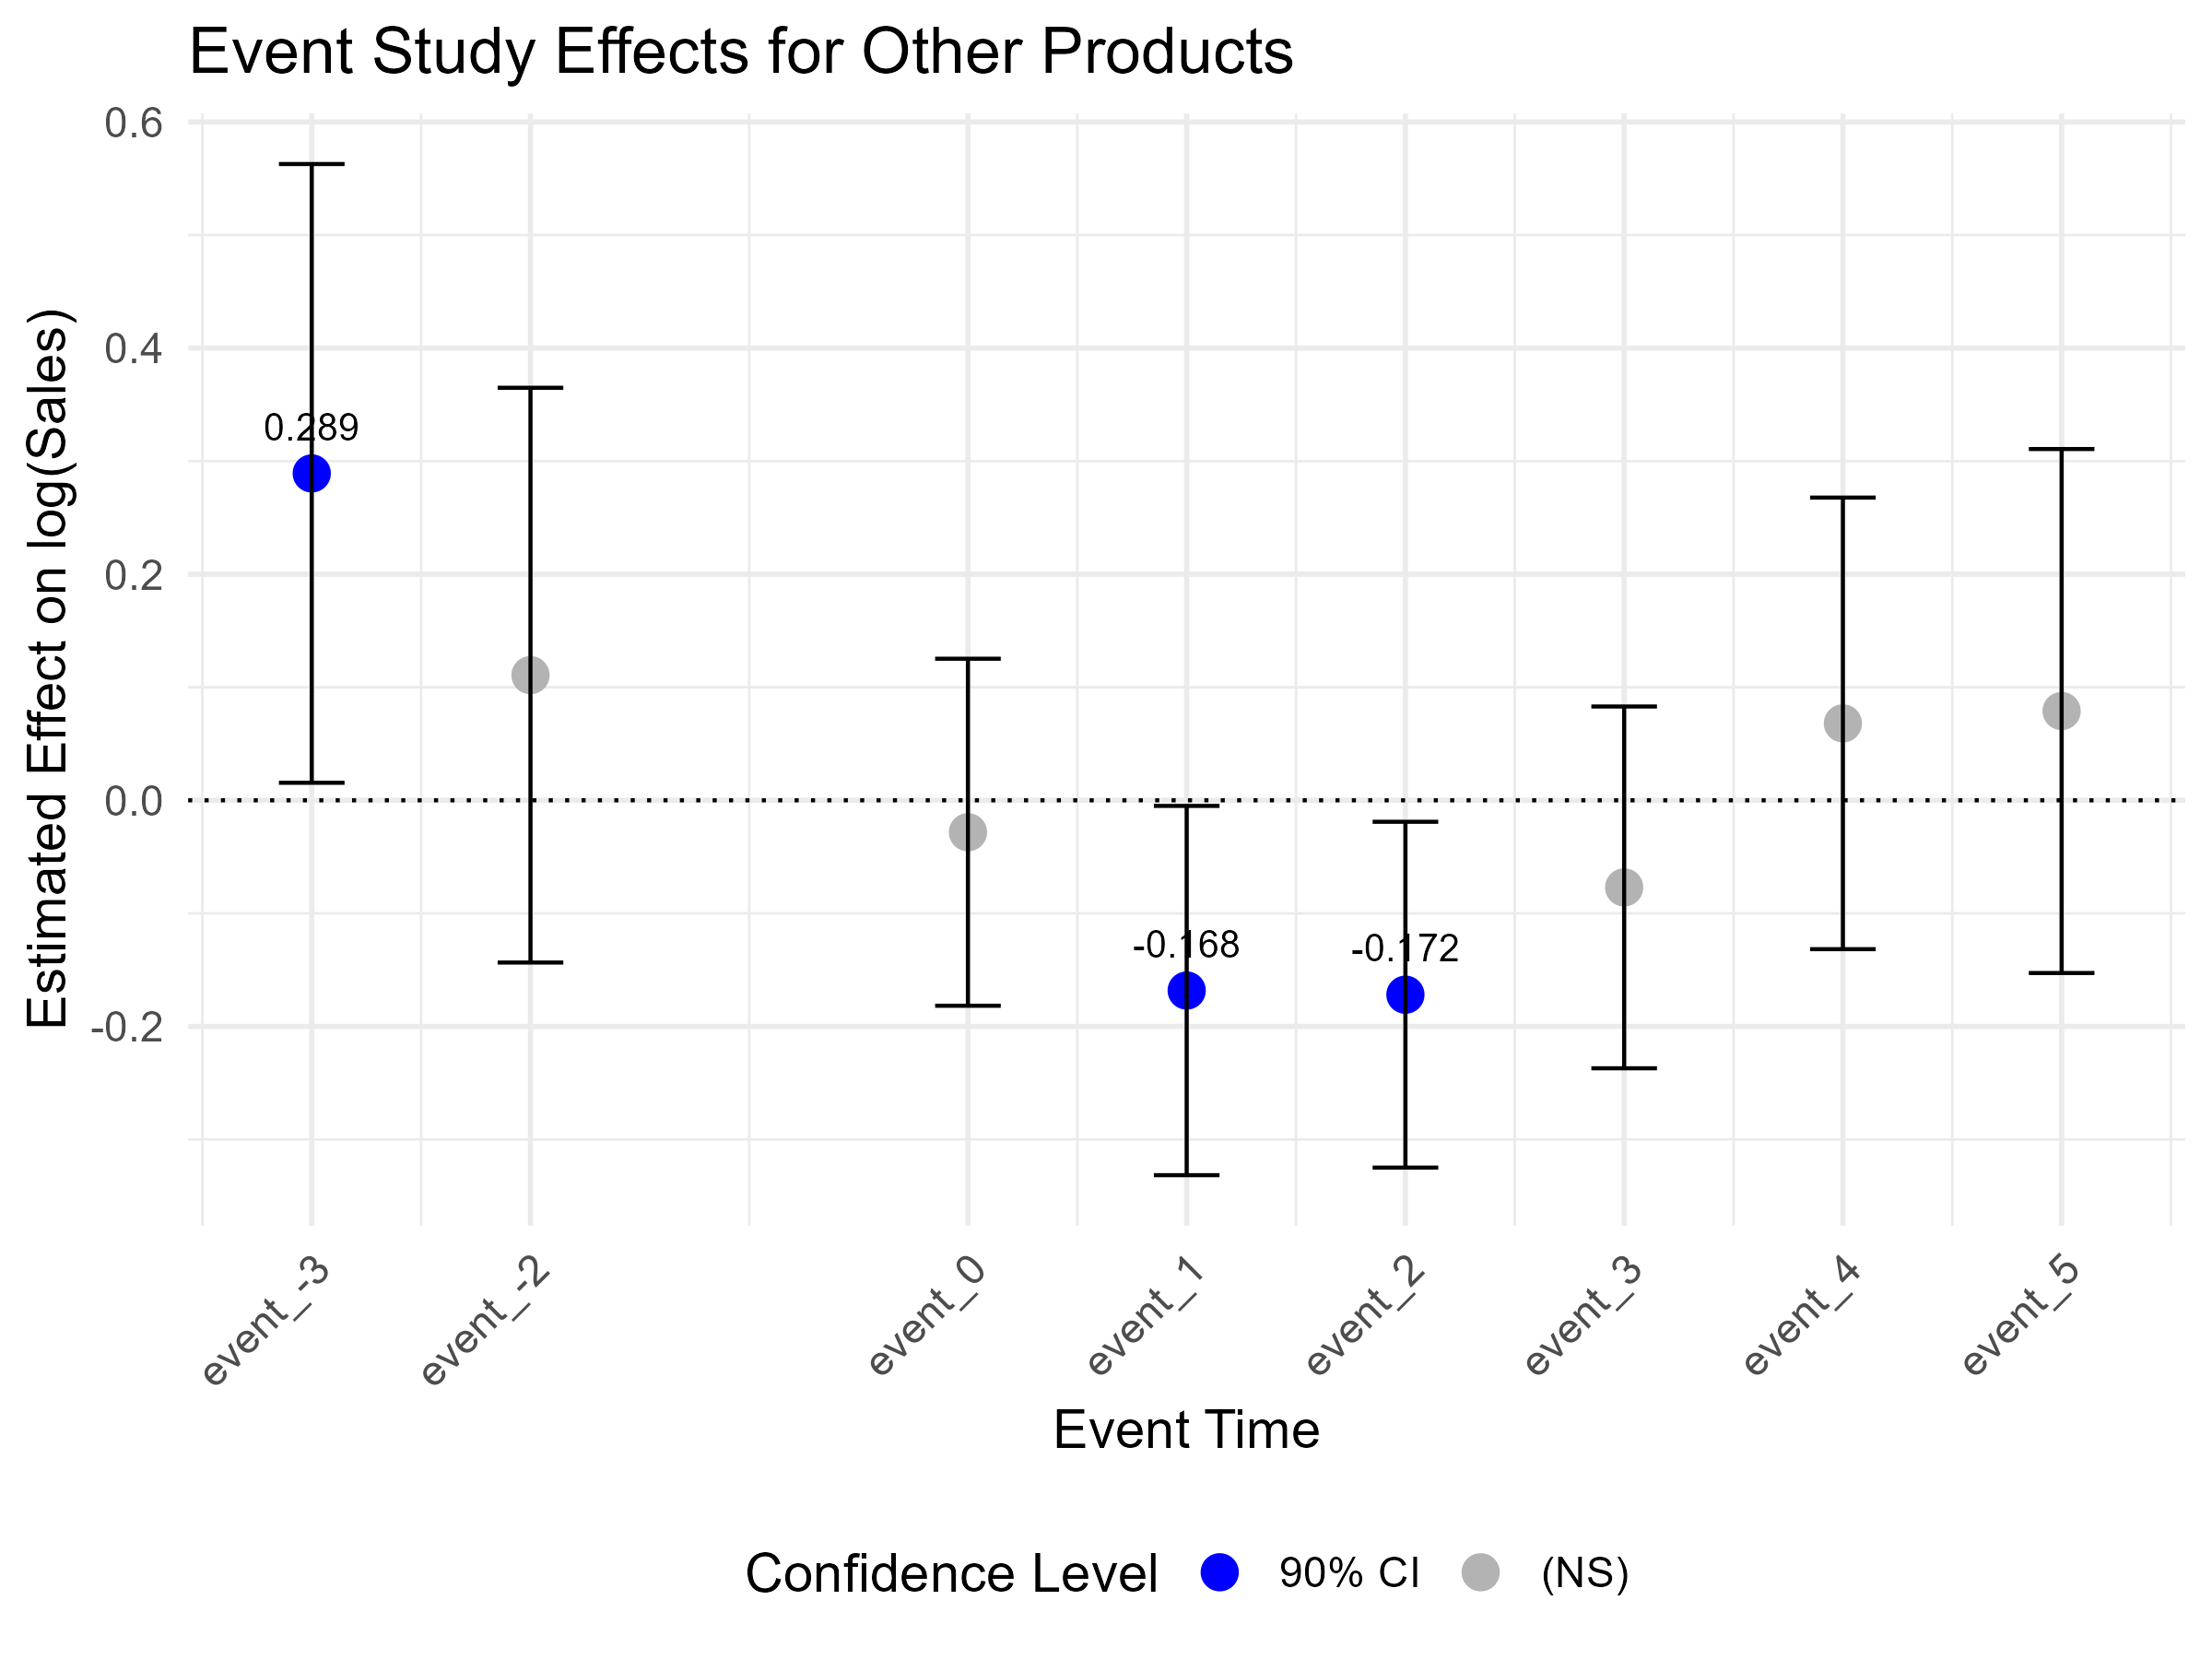
\includegraphics[width=0.55\linewidth]{BaselineOther.png}
        \caption{Impact of Extreme Natural Disasters on Light Manufacturing firms}
        \label{fig:BaselineOthers}
    \end{figure}

\subsection*{Baseline coefficients for Importers regressions}

\begin{table}[H]\centering
\caption{Event Study: Differential Impact on Importers Sales Baseline}
\label{tab:main_interactions_baseline}
\begin{tabular}{lccccc}
\toprule
 & Raw Materials & Intermediate & Finished & Capital & All Importers \\
\textit{Estimation Results} & (1) & (2) & (3) & (4) & (5) \\
\midrule
\multicolumn{6}{l}{\textit{Immediate Effect}} \\
event\_0 & -0.0333 & -0.0343 & 0.0083 & -0.0134   & -0.0318 \\
                    & (0.0464)       & (0.0593)     & (0.0421)       & (0.0509)     & (0.0610)     \\
\midrule
\multicolumn{6}{l}{\textit{Short-Term Effect}} \\
event\_1 & -0.553$^{*}$ & -0.0630 & 0.0122 & -0.0276 & -0.0638 \\
                    & (0.0220)       & (0.0355)       & (0.0316)        & (0.0337)       & (0.0382)     \\
event\_2 & -0.0016 & 0.0056  & 0.0519 & 0.0324   & 0.0087 \\
                    & (0.0288)       & (0.0340)       & (0.0279)        & (0.0325)       & (0.0382)     \\
\midrule
\multicolumn{6}{l}{\textit{Medium/Long Term Effect}} \\
event\_3 & -0.0179   & -0.0386$^{***}$ & 0.0244** & -0.0014         & -0.0421$^{***}$ \\
                    & (0.0176)       & (0.0112)       & (0.0081)        & (0.0155)       & (0.0096)     \\
event\_4 & -0.0283 & -0.0190 & 0.0247*         & 0.0059   & -0.0194 \\
                    & (0.0193)       & (0.0121)       & (0.0107)        & (0.0122)       & (0.0177)     \\
event\_5 & 0.0129         & 0.0094         & 0.0177*         & 0.0057         & 0.0079       \\
                    & (0.0242)       & (0.0378)       & (0.0073)        & (0.0263)       & (0.0390)     \\
\midrule
\multicolumn{6}{l}{\textit{Controls}} \\
tfp\_lp            & 0.7032$^{***}$ & 0.7007$^{***}$ & 0.7030$^{***}$ & 0.7022$^{***}$ & 0.7017$^{***}$ \\
                   & (0.0363)       & (0.0378)       & (0.0368)       & (0.0375)       & (0.0363)       \\
lelectricity       & 0.6748$^{***}$ & 0.6727$^{***}$ & 0.6745$^{***}$ & 0.6752$^{***}$ & 0.6736$^{***}$ \\
                   & (0.0154)       & (0.0185)       & (0.0162)       & (0.0160)       & (0.0154)       \\
lasset             & 0.0003         & 0.0002         & 0.0003         & 0.0003         & 0.0003         \\
                   & (0.0003)       & (0.0004)       & (0.0003)       & (0.0003)       & (0.0003)       \\
lleverage          & 0.0159         & 0.0157         & 0.0160         & 0.0158         & 0.0159         \\
                   & (0.0108)       & (0.0110)       & (0.0110)       & (0.0111)       & (0.0109)       \\
\midrule
Observations       & 8,830          & 8,830          & 8,830          & 8,830          & 8,830          \\
R$^2$              & 0.9654         & 0.9655         & 0.9648         & 0.9654         & 0.9655         \\
Within R$^2$       & 0.6045         & 0.6061         & 0.5975         & 0.6047         & 0.6058         \\
Fixed Effects      & \multicolumn{5}{c}{Firm and Industry-Year and Group-Year} \\
Standard Errors    & \multicolumn{5}{c}{Conley (690 km)} \\
\bottomrule
\end{tabular}
\begin{tablenotes}
\small
\item \textit{Note:} This table presents the Baseline effects of the regressions in table \ref{tab:main_interactions}. The outcome variable is the log of sales. Conley Standard errors (in parentheses). Control variables include: Productivity, leverage ratio, energy expenses, anticipation behaviors variables. Significance levels: $^{.}p<0.1$, $^{*}p<0.05$, $^{**}p<0.01$, $^{***}p<0.001$.
\end{tablenotes}
\end{table}

\subsection*{Regression tables for Alternative Outcomes}

\begin{table}[H]
    \centering
    \small
    \caption{Event Study with Sector Interactions on Log Wages}
    \resizebox{\textwidth}{!}{
    \begin{threeparttable}
    \begin{tabular}{lccccc}
    \toprule
     & Main Effect & Primary \& Processed & Light Manufacturing & Machinery \& Capital & Other \\
    \cmidrule{2-6}
     \textit{Estimation Results} & (1) & (2) & (3) & (4) & (5) \\
    \midrule
    \textit{\textbf{Immediate Impact}} \\
    Event\_0   & 0.0513*  & -0.0334    & -0.2774*** & -0.0448     & 0.0479 \\
              & (0.0233) & (0.0341)   & (0.0234)   & (0.0307)    & (0.1052) \\
    \midrule
    \textit{\textbf{Short term}} \\
    Event\_1   & 0.0830*  & -0.1563*   & -0.3068*** & -0.0932***  & -0.0973 \\
              & (0.0423) & (0.0642)   & (0.0505)   & (0.0170)    & (0.0821) \\
    Event\_2   & 0.0494   & -0.0918**  & -0.1498*** & -0.0405**   & -0.0486. \\
              & (0.0345) & (0.0292)   & (0.0309)   & (0.0153)    & (0.0288) \\
    \midrule
    \textit{\textbf{Medium/Long term}} \\
    Event\_3   & 0.0014   & -0.0195    & -0.0083    & 0.0605*     & -0.0404** \\
              & (0.0126) & (0.0122)   & (0.0241)   & (0.0251)    & (0.0136) \\
    Event\_4   & -0.0228. & 0.0047     & -0.0078    & 0.1703***   & 0.0088 \\
              & (0.0124) & (0.0197)   & (0.0193)   & (0.0135)    & (0.0675) \\
    Event\_5   & -0.0111  & 0.0016     & 0.0002     & 0.1016***   & -0.0437* \\
              & (0.0278) & (0.0490)   & (0.0339)   & (0.0299)    & (0.0182) \\
    \midrule
    \textit{\textbf{Controls}} \\
    Log Leverage Ratio & \multicolumn{5}{c}{-0.1787***} \\
                       & \multicolumn{5}{c}{(0.0330)} \\
    Log Electricity Expenses & \multicolumn{5}{c}{0.4798***} \\
                             & \multicolumn{5}{c}{(0.0204)} \\
    Log Assets & \multicolumn{5}{c}{4.73e-5*} \\
               & \multicolumn{5}{c}{(1.84e-5)} \\
    Droughts cumulative & \multicolumn{5}{c}{0.0016} \\
                        & \multicolumn{5}{c}{(0.0047)} \\
    Floods cumulative & \multicolumn{5}{c}{0.0081} \\
                      & \multicolumn{5}{c}{(0.0053)} \\
    Cyclones cumulative & \multicolumn{5}{c}{-0.0129***} \\
                        & \multicolumn{5}{c}{(0.0030)} \\
    \midrule
    \textbf{Fixed Effects} & \multicolumn{5}{c}{Firm and Industry-Year and Group_Year} \\
    \textbf{Standard Errors} & \multicolumn{5}{c}{Conley (690 km)} \\
    \textbf{Observations} & \multicolumn{5}{c}{8,830} \\
    \textbf{R\textsuperscript{2}} & \multicolumn{5}{c}{0.97358} \\
    \textbf{Within R\textsuperscript{2}} & \multicolumn{5}{c}{0.46456} \\
    \bottomrule
    \end{tabular}
    \begin{tablenotes}
        \small
        \item \textit{Notes:} This table presents the effect of natural disasters on firms wages per sector. Column (1) shows the main treatment effect for the reference sector (Chemicals and Minerals). Columns (2)–(5) show the interaction effects by sector. The omitted category is the reference sector. Controls included are: Productivity, Electricity expenses, leverage ratio, droughts, floods and cyclones cumulative.
        Conley-adjusted standard errors (690 km) are in parentheses.
        \textbf{***} $p<0.001$, \textbf{**} $p<0.01$, \textbf{*} $p<0.05$, \textbf{.} $p<0.1$.
    \end{tablenotes}
    \end{threeparttable}
    }
    \label{tab:event_sector_interaction_wages}
\end{table}

\begin{table}[H]
    \centering
    \small
    \caption{Event Study with Sector Interactions on Log TFP (LP method)}
    \resizebox{\textwidth}{!}{
    \begin{threeparttable}
    \begin{tabular}{lccccc}
    \toprule
     & Main Effect & Primary \& Processed & Light Manufacturing & Machinery \& Capital & Other \\
    \cmidrule{2-6}
     \textit{Estimation Results} & (1) & (2) & (3) & (4) & (5) \\
    \midrule
    \textit{\textbf{Immediate Impact}} \\
    Event\_0   & -0.0745*** & 0.0232     & 0.0670*** & 0.0673     & 0.0619 \\
              & (0.0181)   & (0.0319)   & (0.0182)   & (0.0434)   & (0.0562) \\
    \midrule
    \textit{\textbf{Short term}} \\
    Event\_1   & 0.0238     & 0.0231     & -0.1508*** & -0.0400    & 0.0199 \\
              & (0.0169)   & (0.0356)   & (0.0182)   & (0.0449)   & (0.0429) \\
    Event\_2   & 0.0178.    & -0.1014*   & -0.1366*** & -0.0181    & -0.0125 \\
              & (0.0096)   & (0.0423)   & (0.0167)   & (0.0417)   & (0.0206) \\
    \midrule
    \textit{\textbf{Medium/Long term}} \\
    Event\_3   & -0.0221    & -0.0956*   & 0.0364**   & -0.0313    & 0.0751*** \\
              & (0.0165)   & (0.0405)   & (0.0116)   & (0.0446)   & (0.0228) \\
    Event\_4   & 0.0043     & -0.0900*** & -0.0728*** & -0.0469    & -0.0196 \\
              & (0.0062)   & (0.0272)   & (0.0103)   & (0.0640)   & (0.0249) \\
    Event\_5   & 0.0125     & -0.0830*   & -0.0984*** & -0.1039*   & -0.0721*** \\
              & (0.0113)   & (0.0342)   & (0.0225)   & (0.0485)   & (0.0133) \\
    \midrule
    \textit{\textbf{Controls}} \\
    Log Leverage Ratio & \multicolumn{5}{c}{-0.0877***} \\
                       & \multicolumn{5}{c}{(0.0265)} \\
    Log Electricity Expenses & \multicolumn{5}{c}{-0.0775***} \\
                             & \multicolumn{5}{c}{(0.0058)} \\
    Log Assets & \multicolumn{5}{c}{-3.33e-6} \\
               & \multicolumn{5}{c}{(1.33e-5)} \\
    Droughts cumulative & \multicolumn{5}{c}{0.0058} \\
                        & \multicolumn{5}{c}{(0.0070)} \\
    Floods cumulative & \multicolumn{5}{c}{-0.0031*} \\
                      & \multicolumn{5}{c}{(0.0013)} \\
    Cyclones cumulative & \multicolumn{5}{c}{-0.0046} \\
                        & \multicolumn{5}{c}{(0.0039)} \\
    \midrule
    \textbf{Fixed Effects} & \multicolumn{5}{c}{Firm and Industry-Year and Group-Year} \\
    \textbf{Standard Errors} & \multicolumn{5}{c}{Conley (690 km)} \\
    \textbf{Observations} & \multicolumn{5}{c}{8,830} \\
    \textbf{R\textsuperscript{2}} & \multicolumn{5}{c}{0.82145} \\
    \textbf{Within R\textsuperscript{2}} & \multicolumn{5}{c}{0.03726} \\
    \bottomrule
    \end{tabular}
    \begin{tablenotes}
        \small
        \item \textit{Notes:} This table presents the effect of natural disasters on firm productivity per sector. Column (1) shows the main treatment effect for the reference sector (Chemicals and Minerals). Columns (2)–(5) show the interaction effects by sector. The omitted category is the reference sector. Controls included are: Productivity, Electricity expenses, leverage ratio, droughts, floods and cyclones cumulative.
        Conley-adjusted standard errors (690 km) are in parentheses.
        \textbf{***} $p<0.001$, \textbf{**} $p<0.01$, \textbf{*} $p<0.05$, \textbf{.} $p<0.1$.
    \end{tablenotes}
    \end{threeparttable}
    }
    \label{tab:event_sector_interaction_tfp}
\end{table}

\begin{table}[H]
    \centering
    \small
    \label{tab:sector_interaction_rawM}
    \caption{Event Study with Sector Interactions on Log Raw Materials}
    \resizebox{\textwidth}{!}{
    \begin{threeparttable}
    \begin{tabular}{lccccc}
    \toprule
     & Main Effect & Primary \& Processed & Light Manufacturing & Machinery \& Capital & Other \\
    \cmidrule{2-6}
     \textit{Estimation Results} & (1) & (2) & (3) & (4) & (5) \\
    \midrule
    \textit{\textbf{Immediate Impact}} \\
    Event\_0   & 0.1130**  & -0.2143*** & -0.2469*** & 0.0824**  & -0.1335*** \\
              & (0.0355)  & (0.0578)   & (0.0299)   & (0.0292)  & (0.0191) \\
    \midrule
    \textit{\textbf{Short term}} \\
    Event\_1   & 0.1328*   & -0.3406*** & -0.2750*** & 0.0568    & -0.1948*** \\
              & (0.0544)  & (0.0215)   & (0.0443)   & (0.0502)  & (0.0211) \\
    Event\_2   & 0.1796*** & -0.2166*   & -0.2905*** & -0.0443   & -0.2160*** \\
              & (0.0432)  & (0.0876)   & (0.0522)   & (0.0624)  & (0.0309) \\
    \midrule
    \textit{\textbf{Medium/Long term}} \\
    Event\_3   & 0.0749*** & -0.1709**  & -0.0863*** & 0.0265    & -0.0610*** \\
              & (0.0041)  & (0.0627)   & (0.0238)   & (0.0162)  & (0.0123) \\
    Event\_4   & 0.0694    & -0.2945*** & -0.1068    & 0.0951    & 0.1239 \\
              & (0.0447)  & (0.0890)   & (0.0663)   & (0.0654)  & (0.1032) \\
    Event\_5   & 0.0698.   & -0.3033*   & -0.0348    & 0.0745.   & 0.1160. \\
              & (0.0378)  & (0.1179)   & (0.1187)   & (0.0397)  & (0.0676) \\
    \midrule
    \textit{\textbf{Controls}} \\
    Log Leverage Ratio         & \multicolumn{5}{c}{-0.3315***} \\
                               & \multicolumn{5}{c}{(0.0547)} \\
    TFP (LP)                   & \multicolumn{5}{c}{-0.1611***} \\
                               & \multicolumn{5}{c}{(0.0398)} \\
    Log Electricity Expenses   & \multicolumn{5}{c}{0.7070***} \\
                               & \multicolumn{5}{c}{(0.0075)} \\
    Log Assets                 & \multicolumn{5}{c}{6.98e-5***} \\
                               & \multicolumn{5}{c}{(1.59e-5)} \\
    Droughts cumulative        & \multicolumn{5}{c}{-0.0050} \\
                               & \multicolumn{5}{c}{(0.0215)} \\
    Floods cumulative          & \multicolumn{5}{c}{0.0313***} \\
                               & \multicolumn{5}{c}{(0.0091)} \\
    Cyclones cumulative        & \multicolumn{5}{c}{-0.0194} \\
                               & \multicolumn{5}{c}{(0.0130)} \\
    \midrule
    \textbf{Fixed Effects}     & \multicolumn{5}{c}{Firm and Industry-Year and Group-Year} \\
    \textbf{Standard Errors}   & \multicolumn{5}{c}{Conley (690 km)} \\
    \textbf{Observations}      & \multicolumn{5}{c}{8,830} \\
    \textbf{R\textsuperscript{2}} & \multicolumn{5}{c}{0.93850} \\
    \textbf{Within R\textsuperscript{2}} & \multicolumn{5}{c}{0.44368} \\
    \bottomrule
    \end{tabular}
    \begin{tablenotes}
        \small
        \item \textit{Notes:} This table presents the effect of natural disasters on firms' raw materials expenses per sector. Column (1) shows the main treatment effect for the reference sector (Chemicals and Minerals). Columns (2)–(5) display sector-specific interactions. Controls included are: Productivity, Electricity expenses, leverage ratio, droughts, floods and cyclones cumulative.
        Conley-adjusted standard errors (690 km) are in parentheses. \textbf{***} $p<0.001$, \textbf{**} $p<0.01$, \textbf{*} $p<0.05$, \textbf{.} $p<0.1$.
    \end{tablenotes}
    \end{threeparttable}
    }
\end{table}

\subsection*{Placebo Tests Results}


\begin{figure}[H]
        \centering
        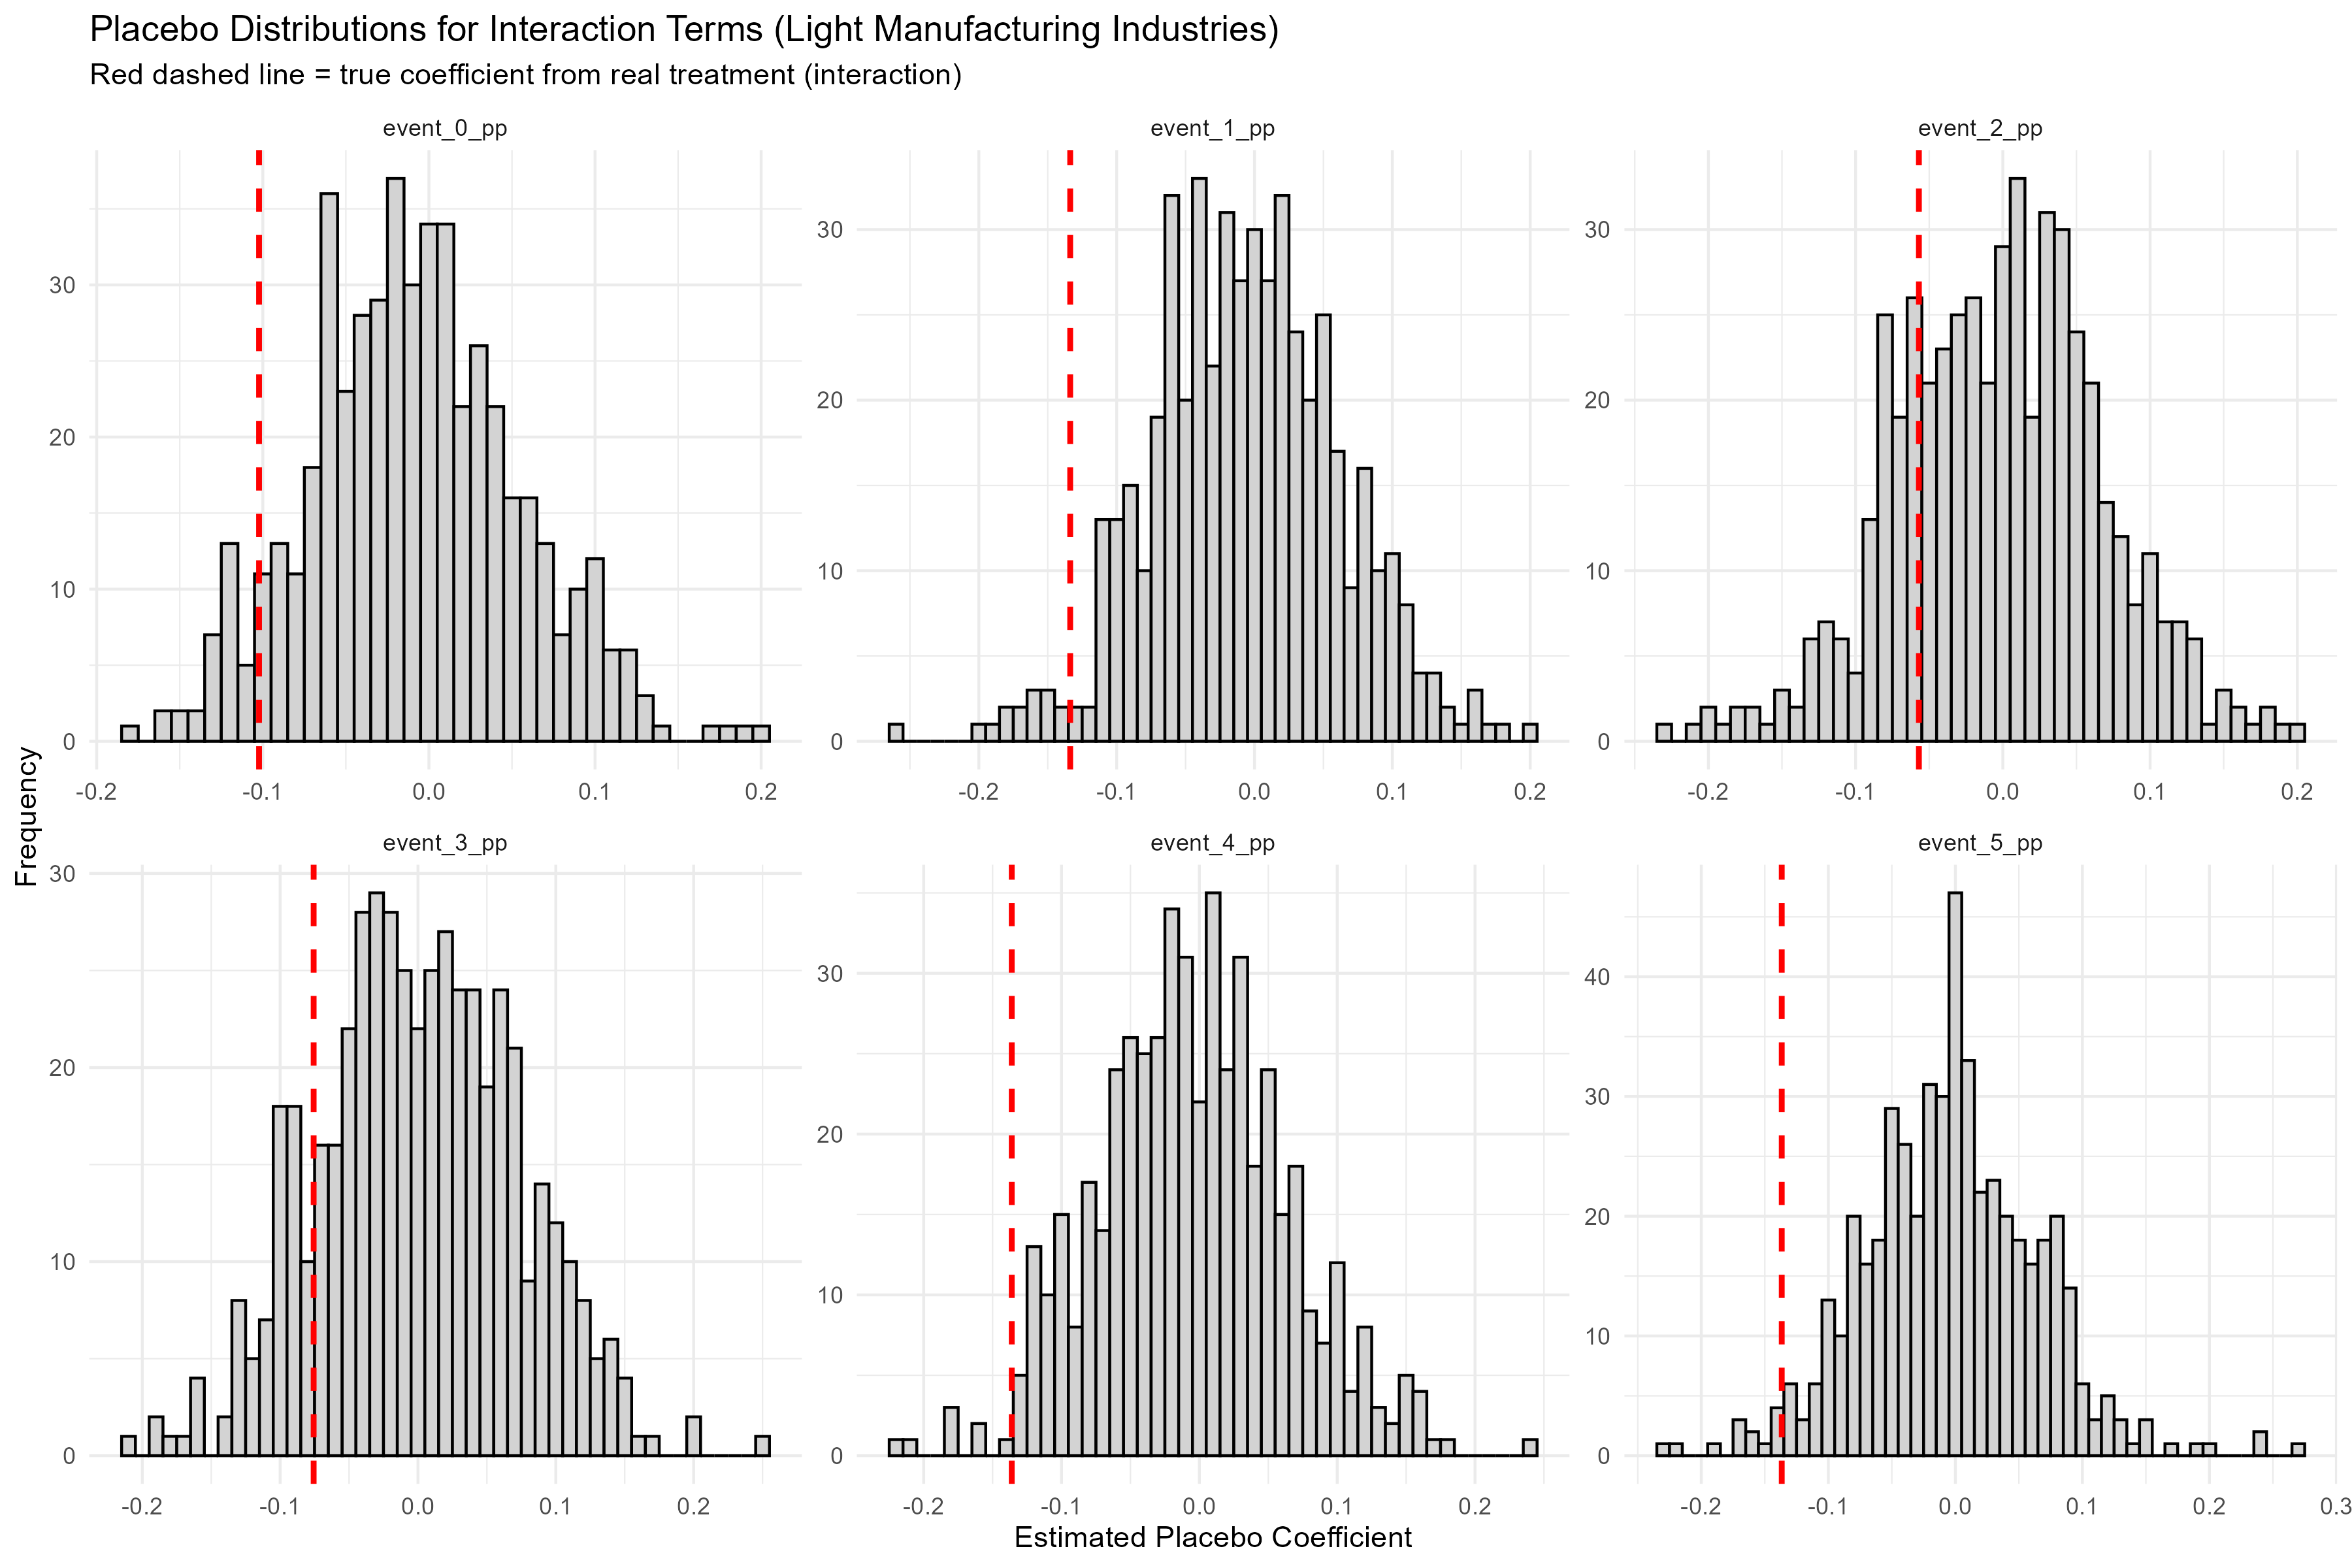
\includegraphics[width=0.85\linewidth]{placebo_LightManuf.png}
        \caption{Distribution of coefficient of Placebo tests for each event period (Light Manufacturing Firms)}
        \label{fig:Placebo_lightmanuf}
    \end{figure}

\begin{figure}[H]
        \centering
        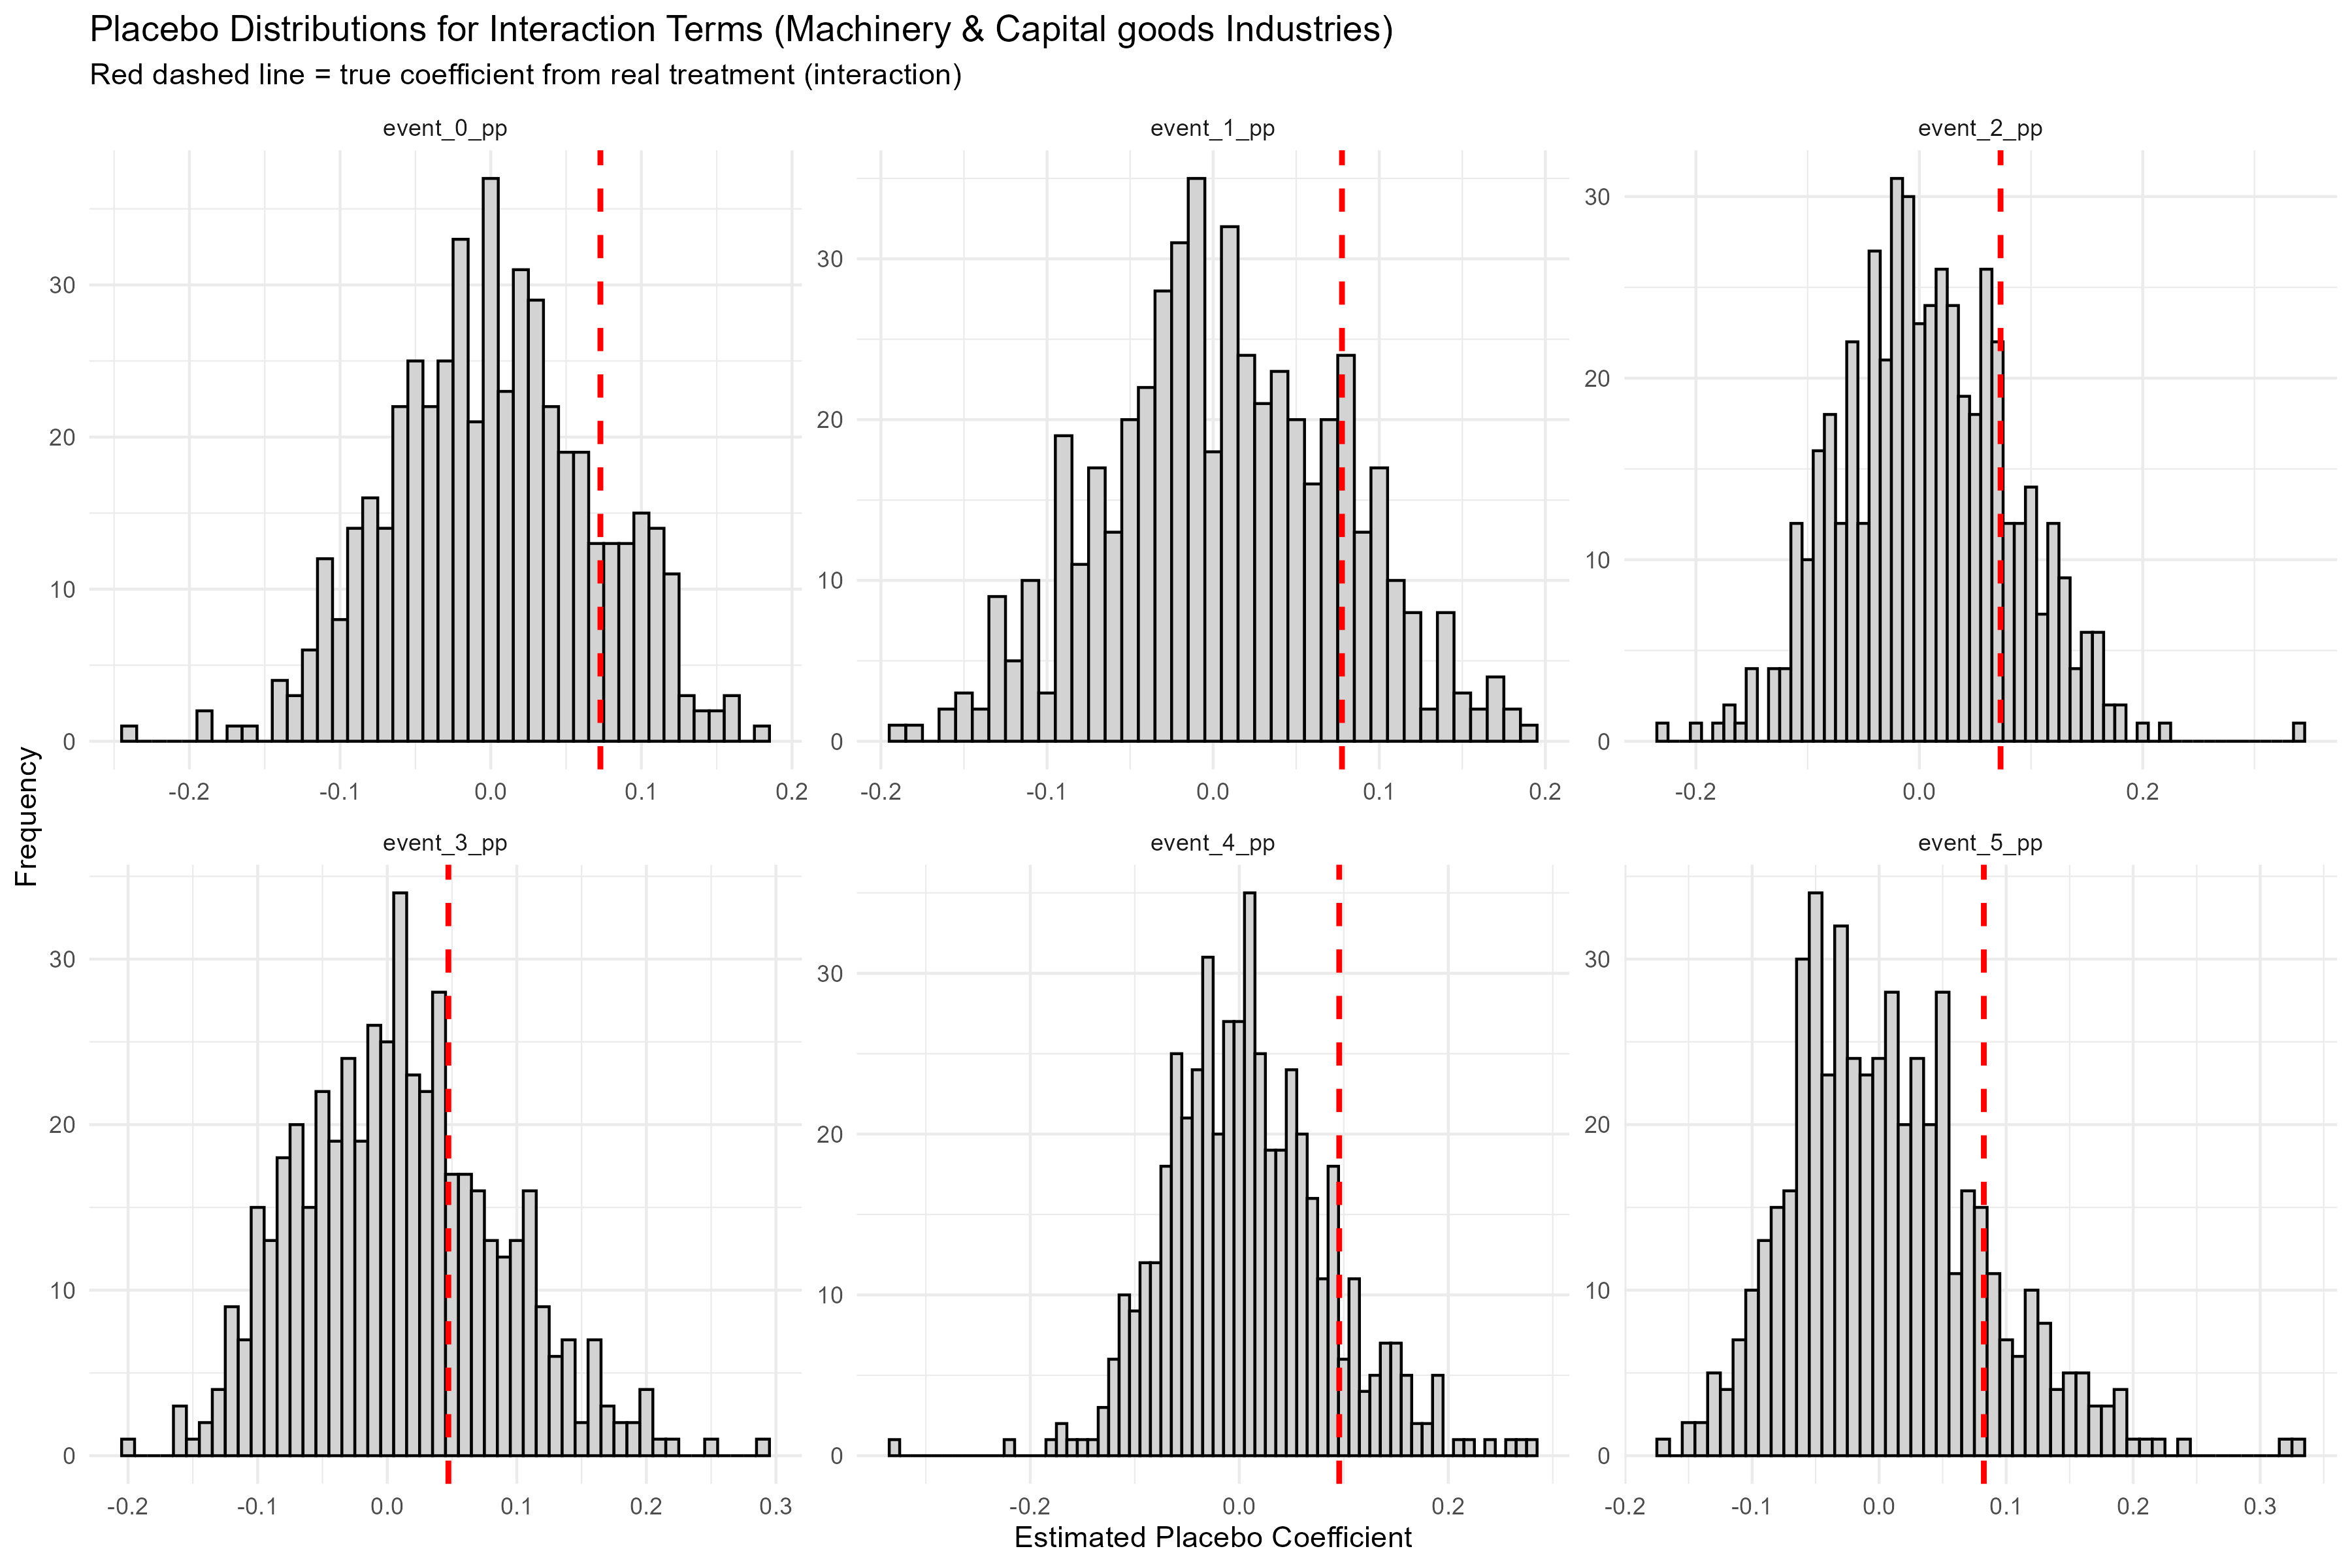
\includegraphics[width=0.85\linewidth]{placebo_Machcap.png}
        \caption{Distribution of coefficient of Placebo tests for each event period (Machinery \& Capital Goods firms)}
        \label{fig:Placebo_machcap}
    \end{figure}

\begin{figure}[H]
        \centering
        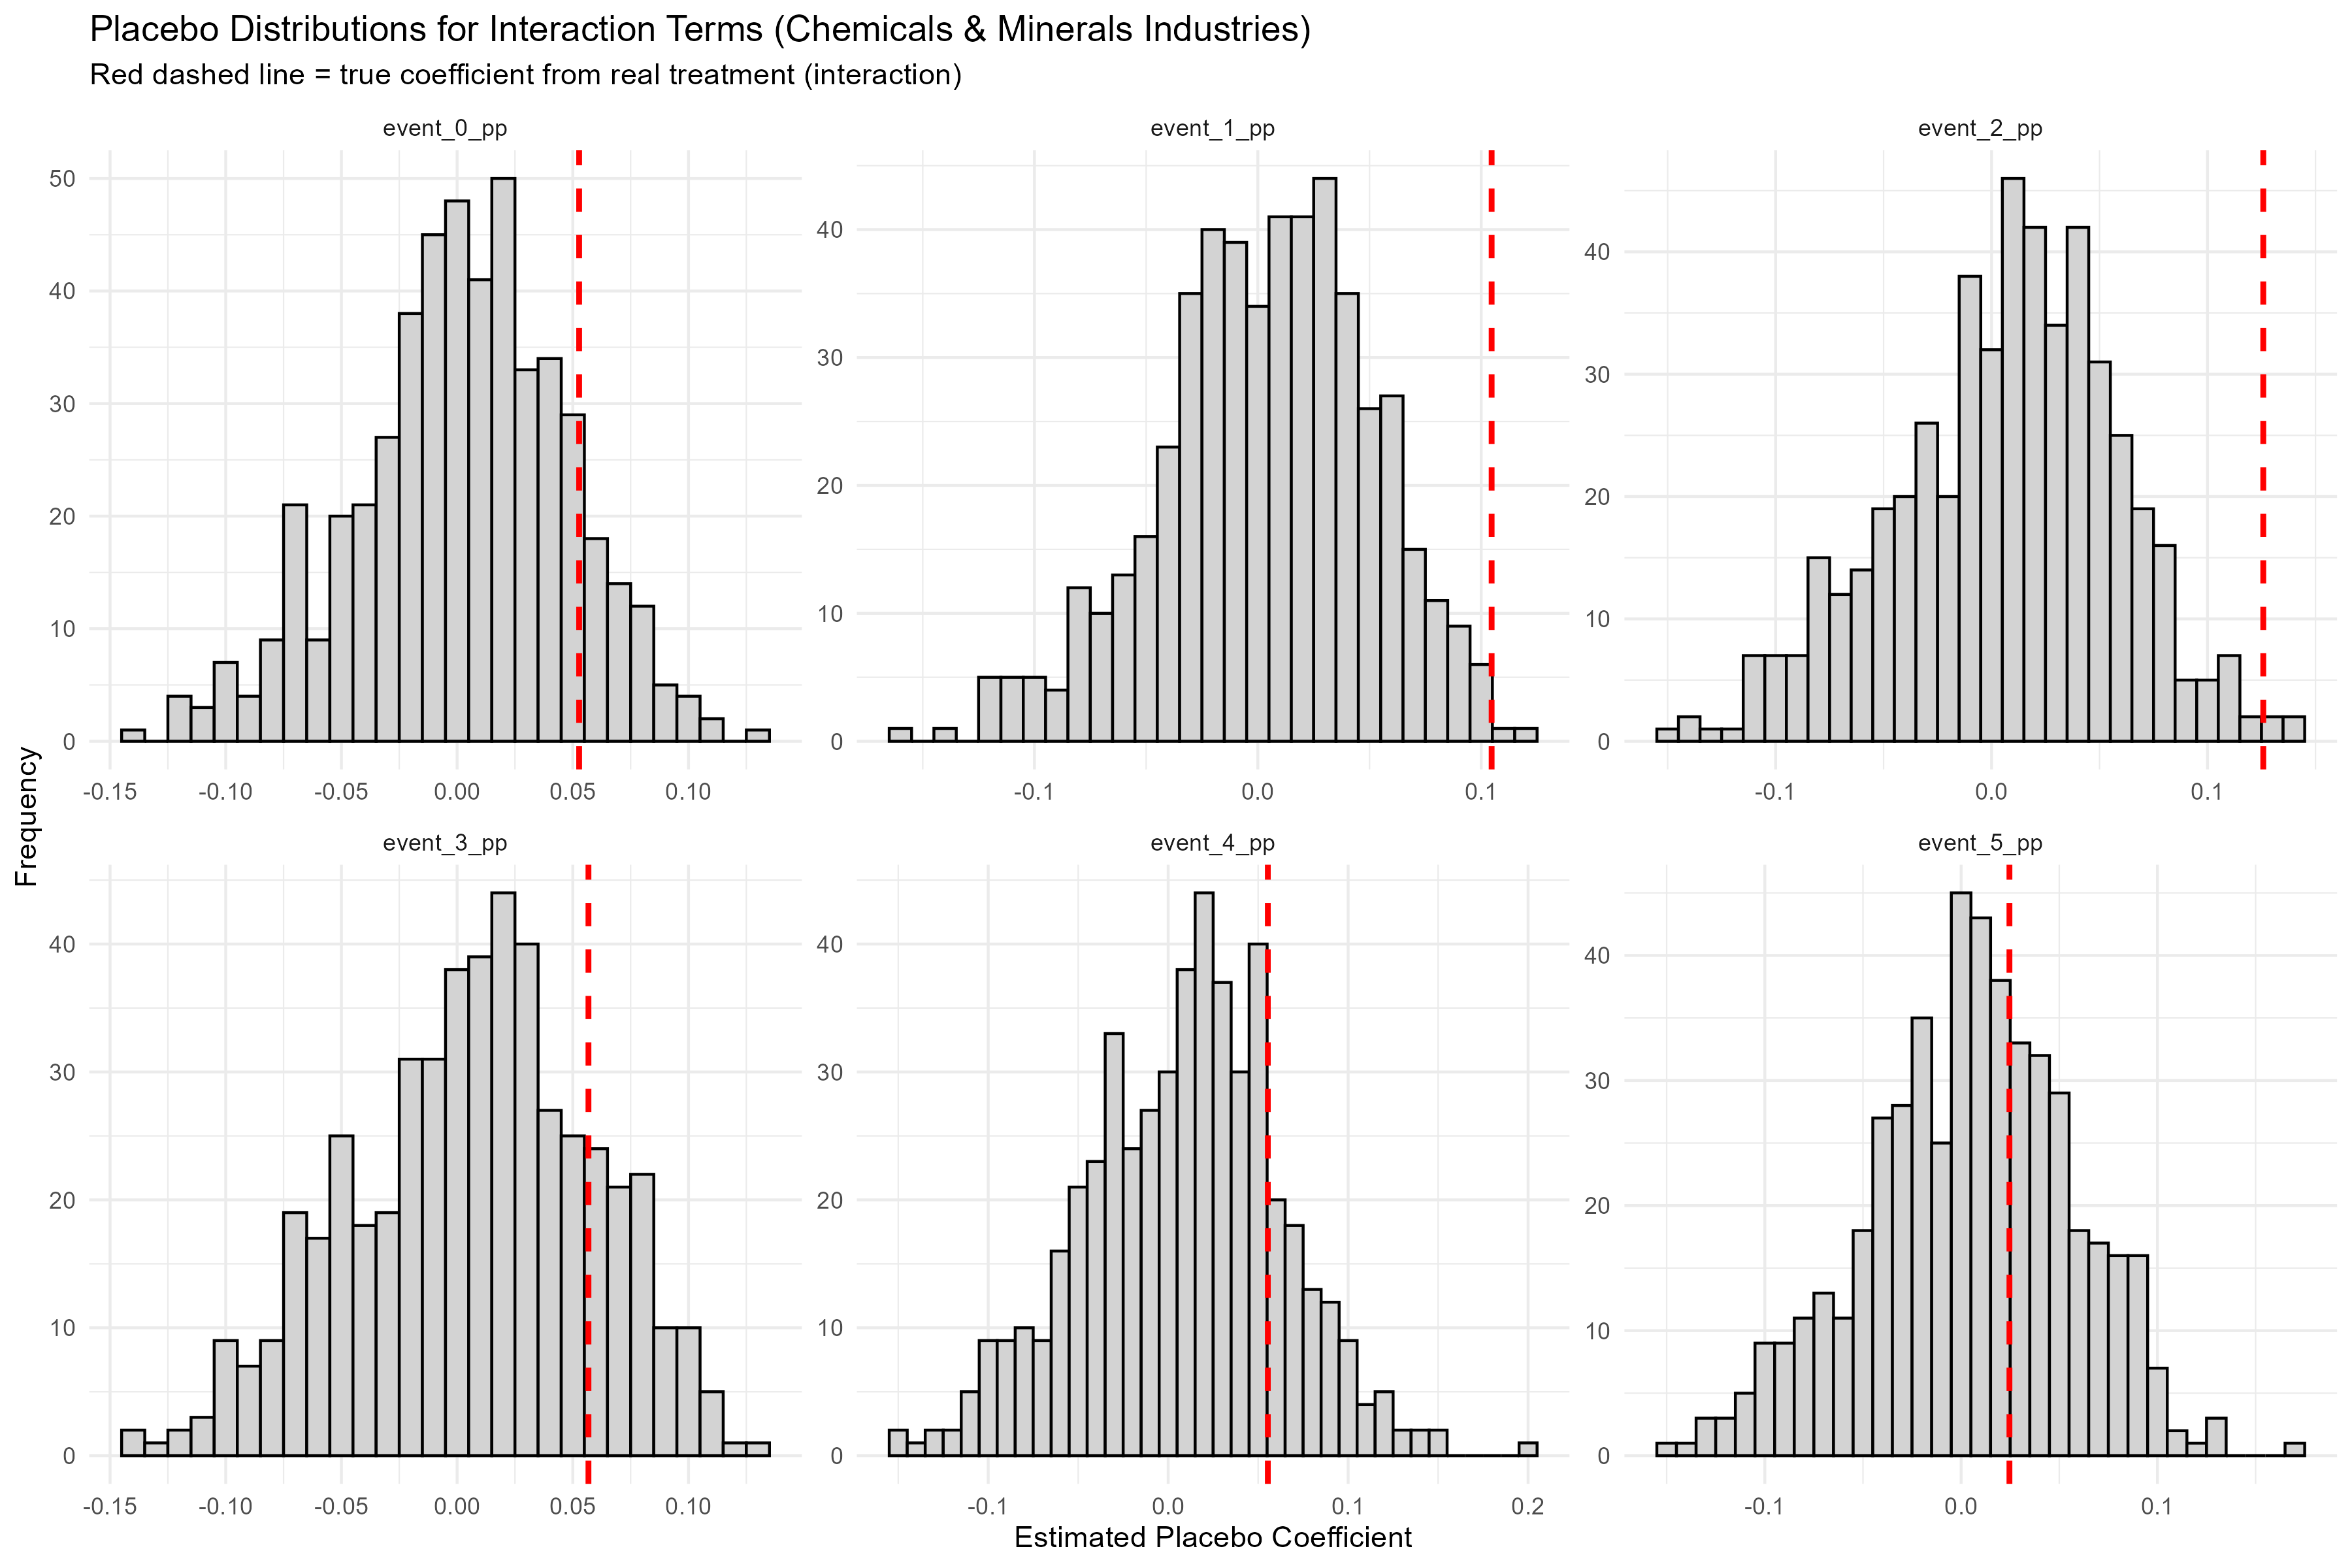
\includegraphics[width=0.85\linewidth]{placebo_ChemMin.png}
        \caption{Distribution of coefficient of Placebo tests for each event period (Chemicals \& Minerals firms)}
        \label{fig:Placebo_chem}
    \end{figure}

\begin{figure}[H]
        \centering
        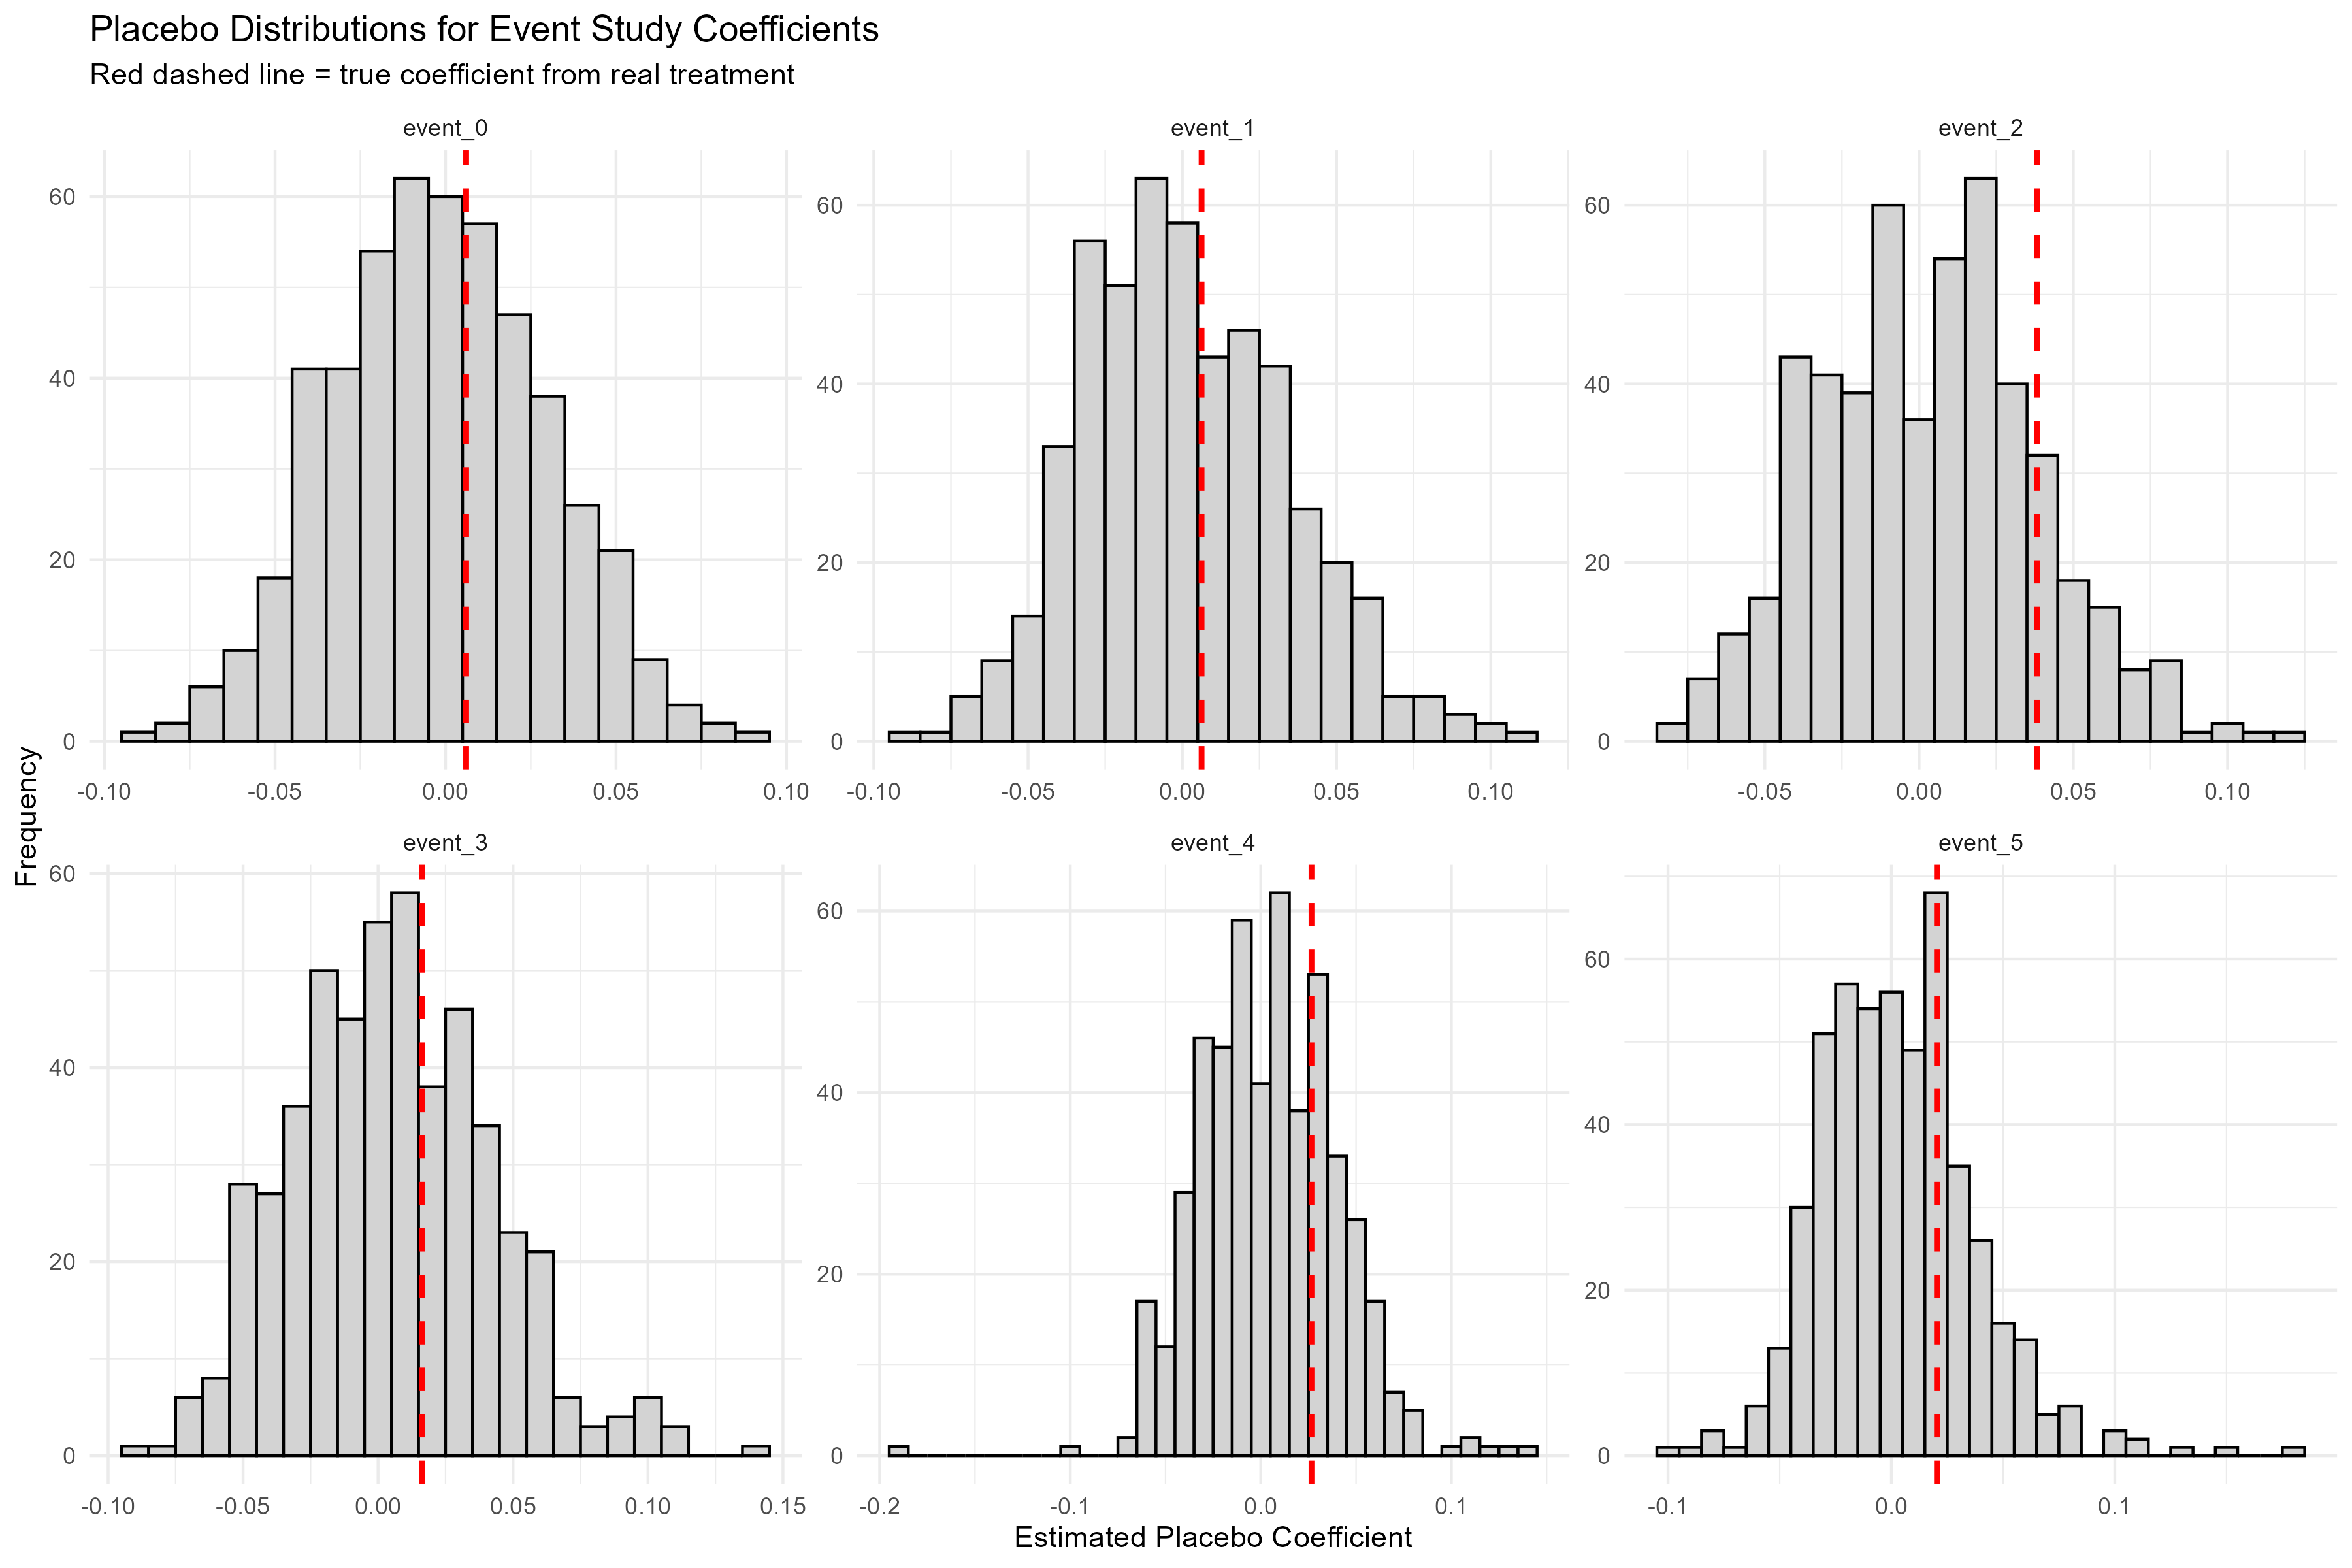
\includegraphics[width=0.85\linewidth]{placebo_test_plot.png}
        \caption{Distribution of coefficient of Placebo tests for each event period}
        \label{fig:Placebo}
    \end{figure}

Table \ref{tab:placebo_pvalues} shows that none of the event time is statistically significant at the conventional thresholds (p-value lower than 0.05). The lowest p-value at the event $\text{t}_{+2}$ could suggest a possible treatment effect two years after the disaster, but it is not conclusive. We can conclude from these tests at an aggregate level that the true estimates are not extreme relative to the placebo distribution and therefore the effect of the disaster could be random.

\begin{table}[H]
\centering
\caption{Empirical p-values from placebo test using random treatment assignment across clusters.}
\begin{tabular}{lcc}
\hline
\textbf{Event Time} & \textbf{True Coefficient} & \textbf{p-value} \\
\hline
event\_0 & 0.0060 & 0.394 \\
event\_1 & 0.0062 & 0.394 \\
event\_2 & 0.0382 & 0.156 \\
event\_3 & 0.0162 & 0.364 \\
event\_4 & 0.0266 & 0.276 \\
event\_5 & 0.0204 & 0.274 \\
\hline
\end{tabular}
\label{tab:placebo_pvalues}
\end{table}

\subsection*{Table of Result for Most Affected Industries}

\begin{table}[htbp]
    \centering
    \small
    \caption{Event Study Sector Interaction Effects on Log Sales (Trend Model)}
    \resizebox{\textwidth}{!}{
    \begin{threeparttable}
    \begin{tabular}{lcccccc}
    \toprule
    \textit{Estimation Results} & \multicolumn{6}{c}{Dependent Variable: Log Sales} \\
    \cmidrule(lr){2-7}
    \textbf{Event Time × Sector} & Food Products & Paper Products & Textiles & Plastic Products & Chemicals & Metal Products \\
    \midrule
    Event\_0   & \textbf{-0.1399***} & \textbf{-0.2528***} & \textbf{-0.2689***} & \textbf{-0.1102***} & \textbf{-0.0767***} & -0.0101 \\
              & (0.0257)    & (0.0187)    & (0.0149)    & (0.0239)  & (0.0231)   & (0.0290)    \\
    Event\_1   & \textbf{-0.1748***} & \textbf{-0.2154***} & \textbf{-0.2559***} & \textbf{-0.1425***} & 0.0354     & 0.0213      \\
              & (0.0142)    & (0.0124)    & (0.0415)    & (0.0296)  & (0.0329)   & (0.0273)    \\
    Event\_2   & -0.1110    & \textbf{-0.1813**}  & \textbf{-0.2395***} & \textbf{-0.1260**}  & 0.0888*    & -0.0017     \\
              & (0.0721)    & (0.0673)    & (0.0477)    & (0.0387)  & (0.0421)   & (0.0151)    \\
    Event\_3   & \textbf{-0.0930**}  & \textbf{-0.1769***} & \textbf{-0.0638***} & \textbf{-0.0858***} & 0.0217*    & \textbf{-0.0221**}   \\
              & (0.0315)    & (0.0280)    & (0.0117)    & (0.0093)  & (0.0104)   & (0.0085)    \\
    Event\_4   & \textbf{-0.1832***} & \textbf{-0.2650**}  & \textbf{-0.1055*}   & 0.0571     & -0.0100    & \textbf{-0.0615**}   \\
              & (0.0318)    & (0.0932)    & (0.0519)    & (0.0641)  & (0.0131)   & (0.0203)    \\
    Event\_5   & \textbf{-0.1313*}   & \textbf{-0.3677***} & -0.0304    & 0.0638     & 0.0526     & \textbf{-0.1423***}  \\
              & (0.0633)    & (0.1115)    & (0.0756)    & (0.0511)  & (0.0424)   & (0.0215)    \\
    \midrule
    \textbf{Fixed Effects}         & \multicolumn{6}{l}{Firms + Industry-Year + Group-Year} \\
    \textbf{Standard Errors}       & \multicolumn{6}{l}{Conley (690km)} \\
    \textbf{Observations}          & \multicolumn{6}{l}{8,830} \\
    \textbf{R\textsuperscript{2}}            & \multicolumn{6}{l}{0.96502} \\
    \textbf{Within R\textsuperscript{2}}     & \multicolumn{6}{l}{0.60027} \\
    \bottomrule
    \end{tabular}
    \begin{tablenotes}
        \small
        \item \textit{Notes:} Each cell displays the coefficient of the interaction between event time and sector. Standard errors are in parentheses and Conley-adjusted with a 690 km cutoff.
        Control variables include: total factor productivity (tfp\_lp), leverage (L\_leverage), electricity use (lelectricity), total assets (assets), and cumulative climate shocks (droughts\_cumulative, floods\_cumulative, cyclones\_cumulative).
        Industry-specific time trends are also controlled for. The omitted (reference) industry is \textbf{Machinery}, so all coefficients are interpreted relative to this group.
        \textbf{***} $p<0.001$, \textbf{**} $p<0.01$, \textbf{*} $p<0.05$, \textbf{.} $p<0.1$.
    \end{tablenotes}
    \end{threeparttable}
    }
    \label{tab:sector_interactions_final_header}
\end{table}

\end{document}
